%\documentclass[newPxFont]{beamer}
%\usetheme{sthlm}
%\documentclass[slidestop,compress,11pt,xcolor=dvipsnames,aspectratio=169]{beamer}
\documentclass[slidestop,compress,11pt,xcolor=dvipsnames]{beamer}
\usepackage[bars]{beamerthemetree} % Beamer theme v 2.2
\usepackage[fontsize=8]{pdfcomment}
\usepackage{colortbl}
\usepackage{multirow}
\newcommand{\pdfnote}[1]{\marginnote{\pdfcomment[icon=note]{#1}}}
\usepackage{kerkis}
\mode<presentation> {
\usefonttheme[onlymath]{serif}
\usetheme{Ilmenau}
\setbeamertemplate{navigation symbols}{} % To remove the navigation symbols from the bottom of all slides uncomment this line
\useinnertheme{circles} %rectangle bullet points instead of circle ones
\useoutertheme[subsection=false]{smoothbars}%Beamer Outer Theme-circles on top
%\setbeamertemplate{footline}[frame number]
}
\newcommand*\oldmacro{}%
\let\oldmacro\insertshorttitle%
\renewcommand*\insertshorttitle{%
\oldmacro\hfill%
\insertframenumber\,}%/\,\inserttotalframenumber

% Creates a slide with the name of the section
%\AtBeginSection[]{
%  \begin{frame}
%  \vfill
%  \centering
%  \begin{beamercolorbox}[sep=8pt,center,shadow=true,rounded=true]{title}
%    \usebeamerfont{title}\insertsectionhead\par%
%  \end{beamercolorbox}
%  \vfill
%  \end{frame}
%}
\graphicspath{{images/}}

%\titlegraphic{
\includegraphics[height=.15\textheight]{logo/fapesp_s}}
\titlegraphic{

\includegraphics[height=.10\textheight]{logo/fapesp_s}
\hspace{1cm}

\includegraphics[height=.08\textheight]{logo/usp}
%\hspace{2cm}
%
\includegraphics[width=1.5cm]{logo/fmrp}
%\hspace{1cm}
}
\usepackage{csvsimple}
\usepackage{multicol}
\usepackage{remreset}% tiny package containing just the \@removefromreset command
\makeatletter
\@removefromreset{subsection}{section}
\makeatother
\setcounter{subsection}{1}

\makeatletter
\setbeamertemplate{footline}
{
\leavevmode%
\hbox{%
\begin{beamercolorbox}[wd=\paperwidth,ht=2.00ex,dp=0.0ex,center]{title in head/foot}%
\usebeamerfont{title in head/foot}Tiago C. Silva | \inserttitle \hspace*{2em}
\insertframenumber{} / \inserttotalframenumber\hspace*{1ex}
\end{beamercolorbox}%
}%
\vskip0pt%
}
\makeatother

\usepackage{csvsimple}
\usepackage{siunitx}
\usepackage{float}
\usepackage{booktabs}
\usepackage{tikz}
\usetikzlibrary{automata}
\usetikzlibrary{shapes.geometric, arrows}
\usetikzlibrary{shadows}
\tikzstyle{start} = [rectangle,minimum size=6mm,rounded corners=3mm,
very thick,draw=black!50, top color=white,bottom color=white,
font=\itshape\footnotesize,drop shadow]
\tikzstyle{fail} = [rectangle, rounded corners, minimum width=3cm, minimum height=1cm,text centered,font=\footnotesize, draw=black, fill=white, text=red,  drop shadow]
\tikzstyle{success} = [rectangle, rounded corners, minimum width=3cm, font=\footnotesize,minimum height=1cm,text centered, draw=black, fill=white, text=green!70!black!100,  drop shadow]
\tikzstyle{process} = [rectangle, rounded corners, minimum width=1cm, minimum height=0.5cm, text centered, text width=5cm, font=\footnotesize,draw=black, fill=white, text=black,drop shadow]
\tikzstyle{decision} = [diamond, minimum width=0.5cm, minimum height=0.5cm,font=\itshape\footnotesize,
text centered, draw=black,top color=white,bottom color =white, text=black, drop shadow]
\tikzstyle{arrow} = [thick,->,>=stealth,-latex',draw,rounded corners]
\tikzstyle{cloud} = [draw, ellipse,rounded corners=3mm,very thick,draw=black!50, top color=white,bottom color=white,font=\itshape\footnotesize,
node distance=4cm,minimum height=1em, drop shadow]
\tikzstyle{analysis} = [rectangle, rounded corners, minimum width=3cm, font=\footnotesize,minimum height=1cm,text centered, draw=black, fill=white, drop shadow]
\tikzstyle{package} = [rectangle, rounded corners, minimum width=3cm, font=\footnotesize,minimum height=1cm,text centered, draw=black, fill=white, drop shadow]

%-=-=-=-=-=-=-=-=-=-=-=-=-=-=-=-=-=-=-=-=-=-=-=-=
%        LOADING PACKAGES
%-=-=-=-=-=-=-=-=-=-=-=-=-=-=-=-=-=-=-=-=-=-=-=-=
\usepackage[utf8]{inputenc}

%-=-=-=-=-=-=-=-=-=-=-=-=-=-=-=-=-=-=-=-=-=-=-=-=
%        BEAMER OPTIONS
%-=-=-=-=-=-=-=-=-=-=-=-=-=-=-=-=-=-=-=-=-=-=-=-=

%\setbeameroption{show notes}

%-=-=-=-=-=-=-=-=-=-=-=-=-=-=-=-=-=-=-=-=-=-=-=-=
%
%	PRESENTATION INFORMATION
%
%-=-=-=-=-=-=-=-=-=-=-=-=-=-=-=-=-=-=-=-=-=-=-=-=

\title{Bioinformatic tool to integrate and understand aberrant epigenomic and genomic changes associated with cancer}
\subtitle{Methods, development and analysis}
%\date{\small{\jobname}}
\date{\today}
\author{\texttt{Tiago Chedraoui Silva}}
\institute{University of São Paulo (USP)}

\begin{document}

%-=-=-=-=-=-=-=-=-=-=-=-=-=-=-=-=-=-=-=-=-=-=-=-=
%
%	TITLE PAGE
%
%-=-=-=-=-=-=-=-=-=-=-=-=-=-=-=-=-=-=-=-=-=-=-=-=

{
\setbeamertemplate{footline}{}
\maketitle
}
%\begin{frame}[plain]
%	\titlepage
%\end{frame}


\section*{Overview}
\begin{frame}{Overview}
 % For longer presentations use hideallsubsections option
 \tableofcontents[hideallsubsections]
\end{frame}


%-=-=-=-=-=-=-=-=-=-=-=-=-=-=-=-=-=-=-=-=-=-=-=-=
%
%	SECTION: BACKGROUND
%
%-=-=-=-=-=-=-=-=-=-=-=-=-=-=-=-=-=-=-=-=-=-=-=-=

\section{Introduction}

\begin{frame}{Context}
\vspace*{-0.5cm}
	\begin{figure}
		\centering
	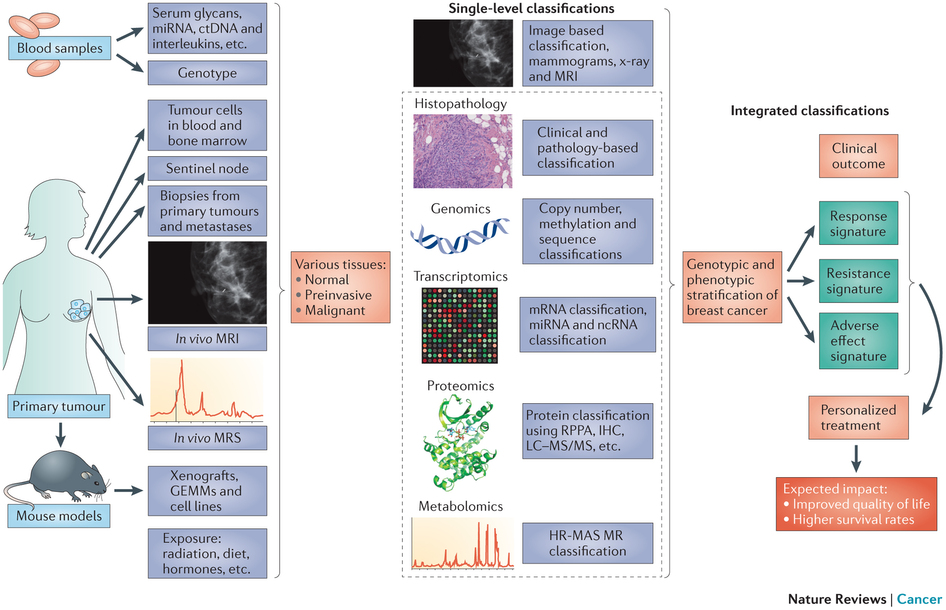
\includegraphics[width=1.0\textwidth]{intro/breast.jpg}{\tiny{\\Kristensen, Vessela N., et al. "Principles and methods of integrative genomic analyses in cancer." Nature Reviews Cancer}}
	\end{figure}
\end{frame}


\begin{frame}{Understand molecular behaviours}
\vspace{-0.4cm}
	\begin{figure}
		\centering
	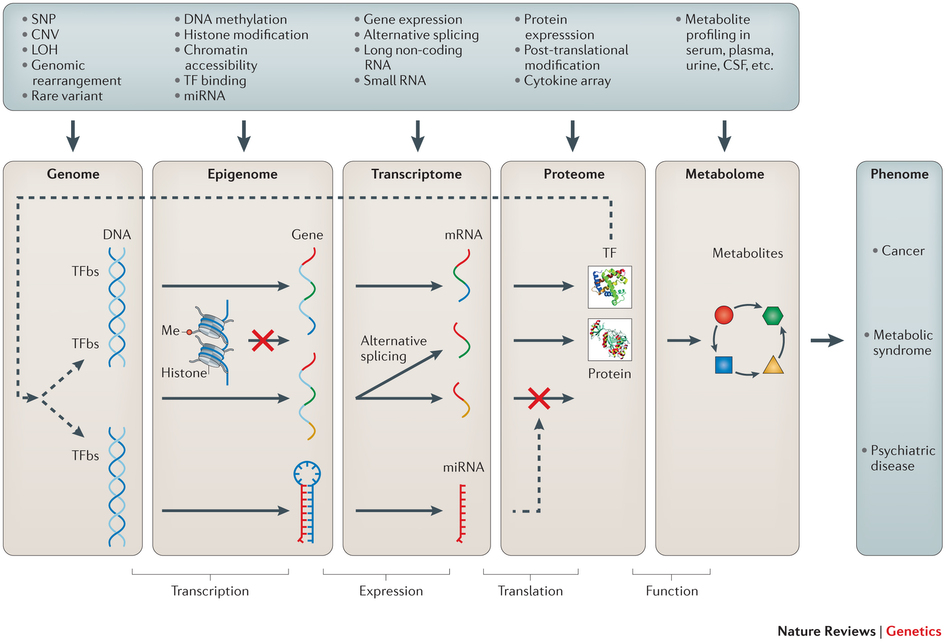
\includegraphics[width=0.8\linewidth,height=0.8\textheight]{intro/data_integration.jpg}{\tiny{\\Ritchie, Marylyn D., et al. "Methods of integrating data to uncover genotype-phenotype interactions." Nature Reviews Genetics}}
	\end{figure}
\end{frame}


\begin{frame}{Integrative statistical analysis}

\begin{block}{Integrative statistical analysis}
Analysis of at least two different types of omics data
% he analysis can be restricted to molecular data (such as in expression quantitative trait loci (eQTL) studies, in which the relation between germ line variation and gene expression is investigated35, 36) or it can involve clinical outcomes (for example, survival, stage and treatment response) or intermediate phenotypes and biomarkers.
\end{block}



\begin{alertblock}{Objectives}
\begin{enumerate}
\item Understand molecular behaviours, mechanisms and relationships between and within the different types of molecular structures
% including associations between these and various phenotypes
\item Understand the taxonomy of diseases, thereby classifying individuals into latent classes of disease subtype
\item Predict an outcome or phenotype (survival, efficacy of therapy) for patients.
\end{enumerate}
\end{alertblock}
\end{frame}

\begin{frame}
\begin{columns}
     \begin{column}{.48\textwidth} % Left column and width
     \begin{block}{Genetics}
     The study of heritable changes in gene activity or function due to the direct alteration of the DNA sequence.
     For example, point mutations, deletions, insertions, and translocation.
     \end{block}
     \end{column}%
     \hfill%
     \begin{column}{.48 \textwidth} % Right column and width
     \begin{alertblock}{Epigenetics}
     The study of changes in gene activity or function not associated with any change of the DNA sequence. For example, DNA methylation and Histone modifications.
     \end{alertblock}
     \end{column}
   \end{columns}

   \begin{exampleblock}{The epigenetic mechanism}
   Even though all cells in an organism contain the same genetic information, the epigenetic mechanism controls which gene are expressed enabling the existence of a diversified gene expression profiles in a variety of cells and tissues in multicellular organisms.
   \end{exampleblock}
\end{frame}

\begin{frame}{Genetics alterations}
\vspace*{-0.5cm}
 \begin{figure}
  \centering
  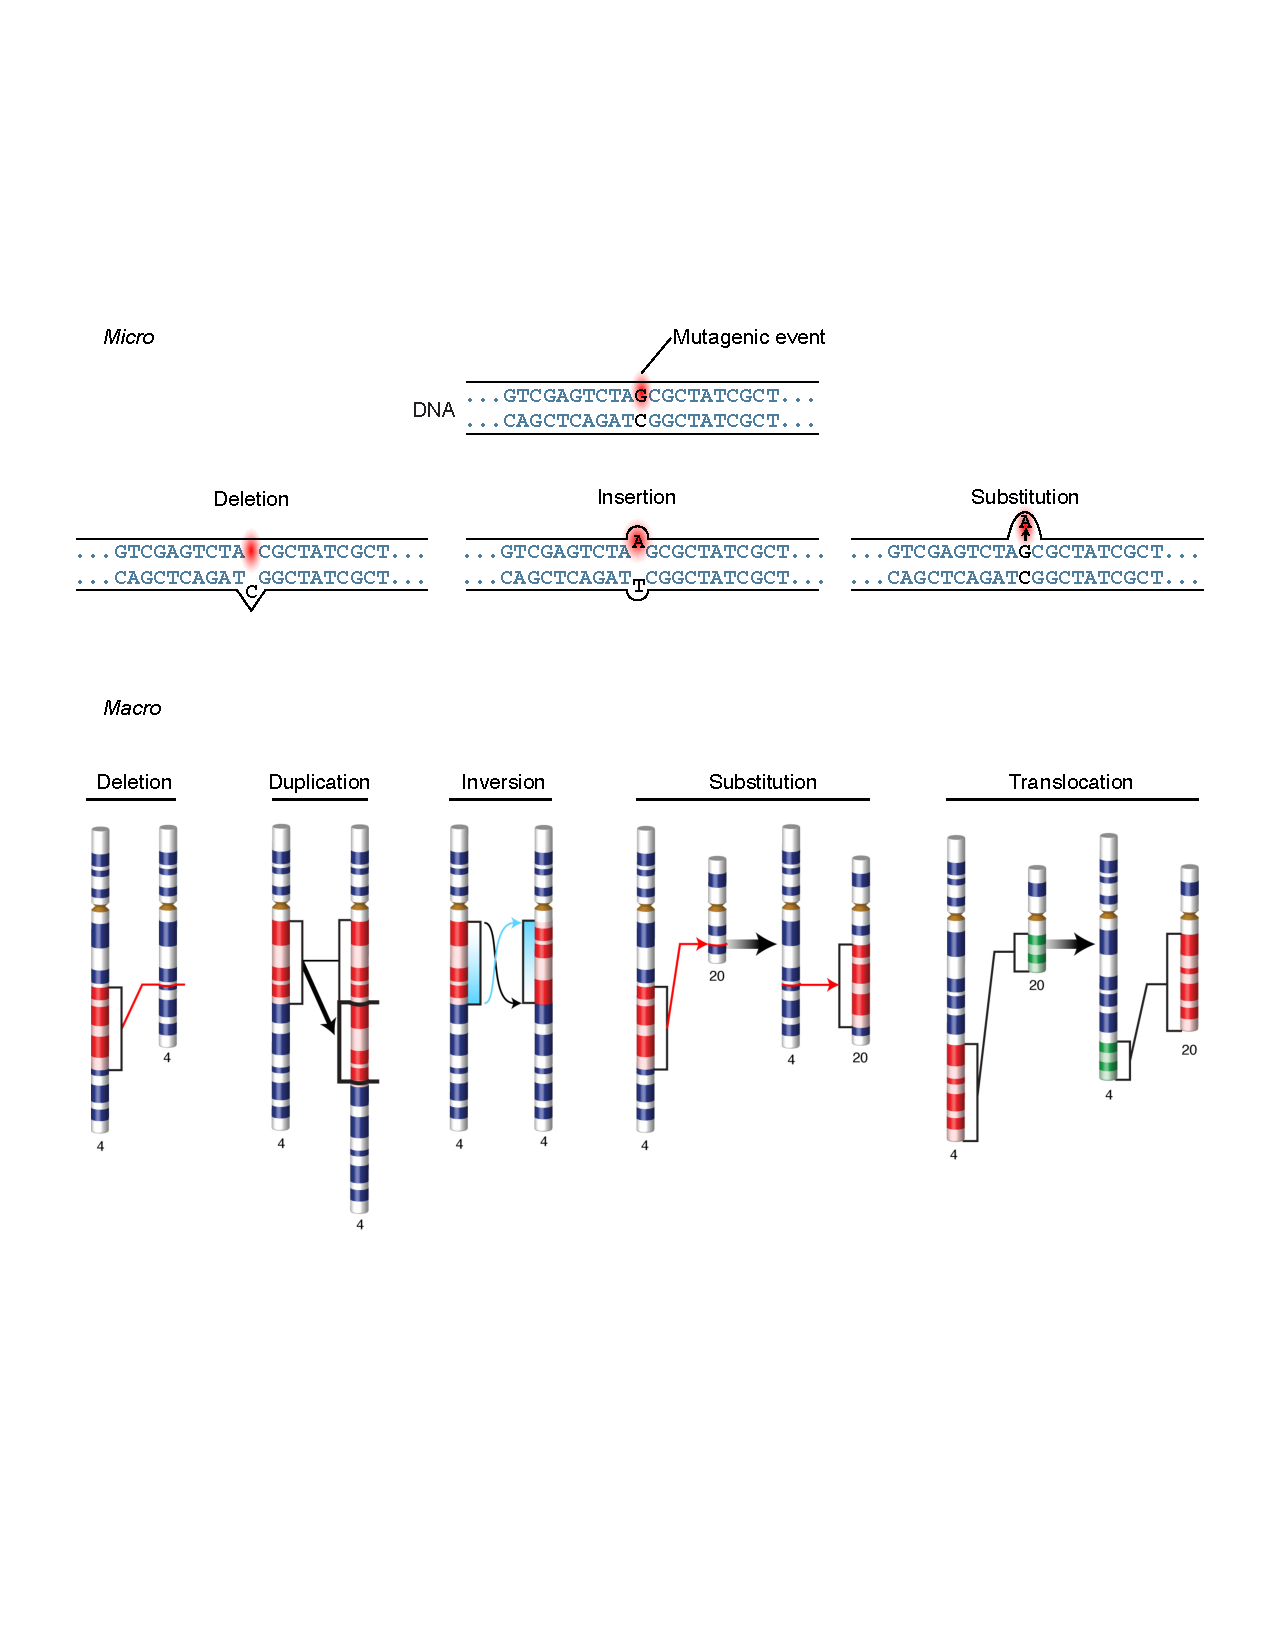
\includegraphics[width=0.9\linewidth]{intro/mutation.pdf}{\tiny{\\Source: National Human Genome Research Institute's Talking Glossary (http://www.genome.gov/glossary/). Accessed: 26-12-2017}}
 \end{figure}
\end{frame}

\begin{frame}{Epigenetic alterations}
\vspace*{-0.5cm}
 \begin{figure}
  \centering
  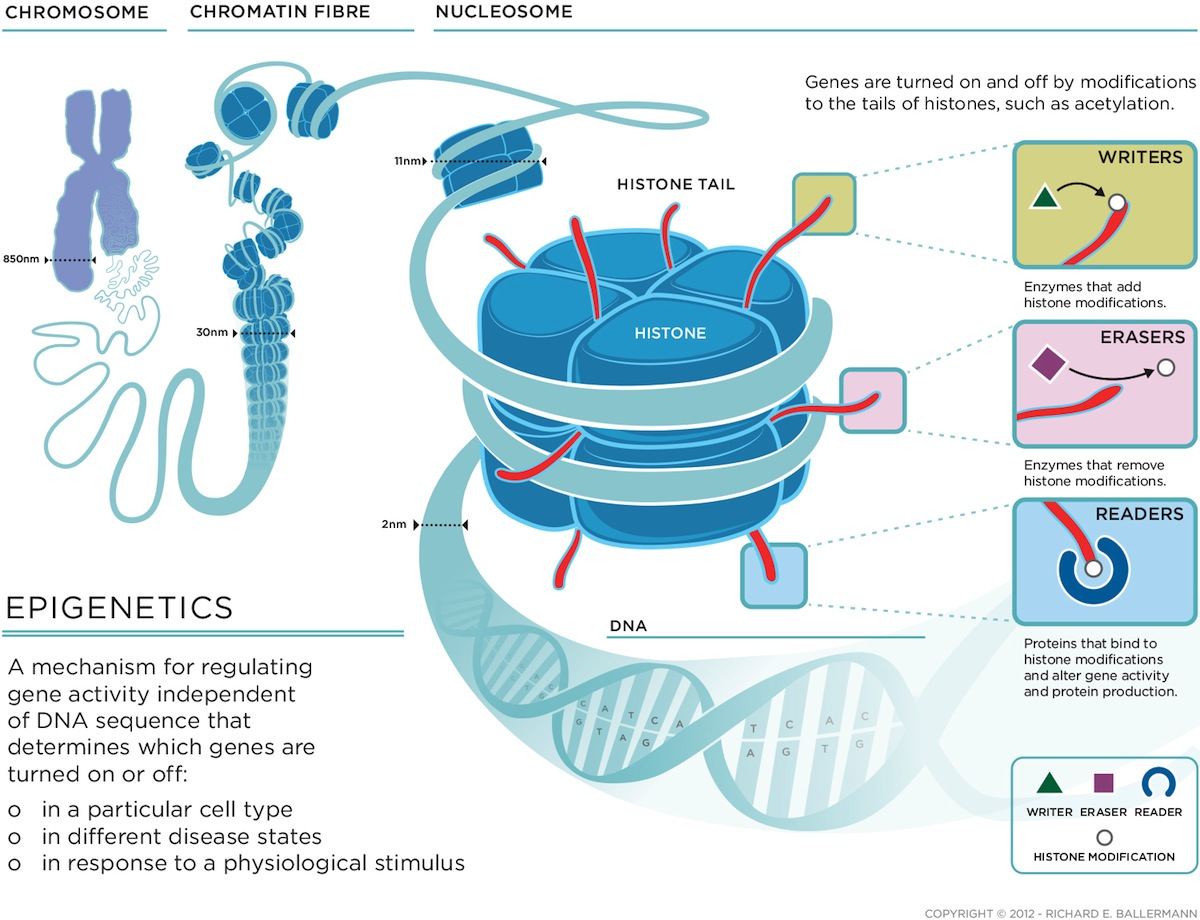
\includegraphics[width=0.9\linewidth]{intro/epigenetics.jpg}{\tiny{\\Source: http://wondergressive.com/epigenetics-key-overcoming-genetic-predisposition/. Accessed: 26-12-2017}}
 \end{figure}
\end{frame}



\begin{frame}[plain]%{Integrative analysis - histone modification}
 \vspace*{-0.5cm}
\begin{figure}
 \centering
 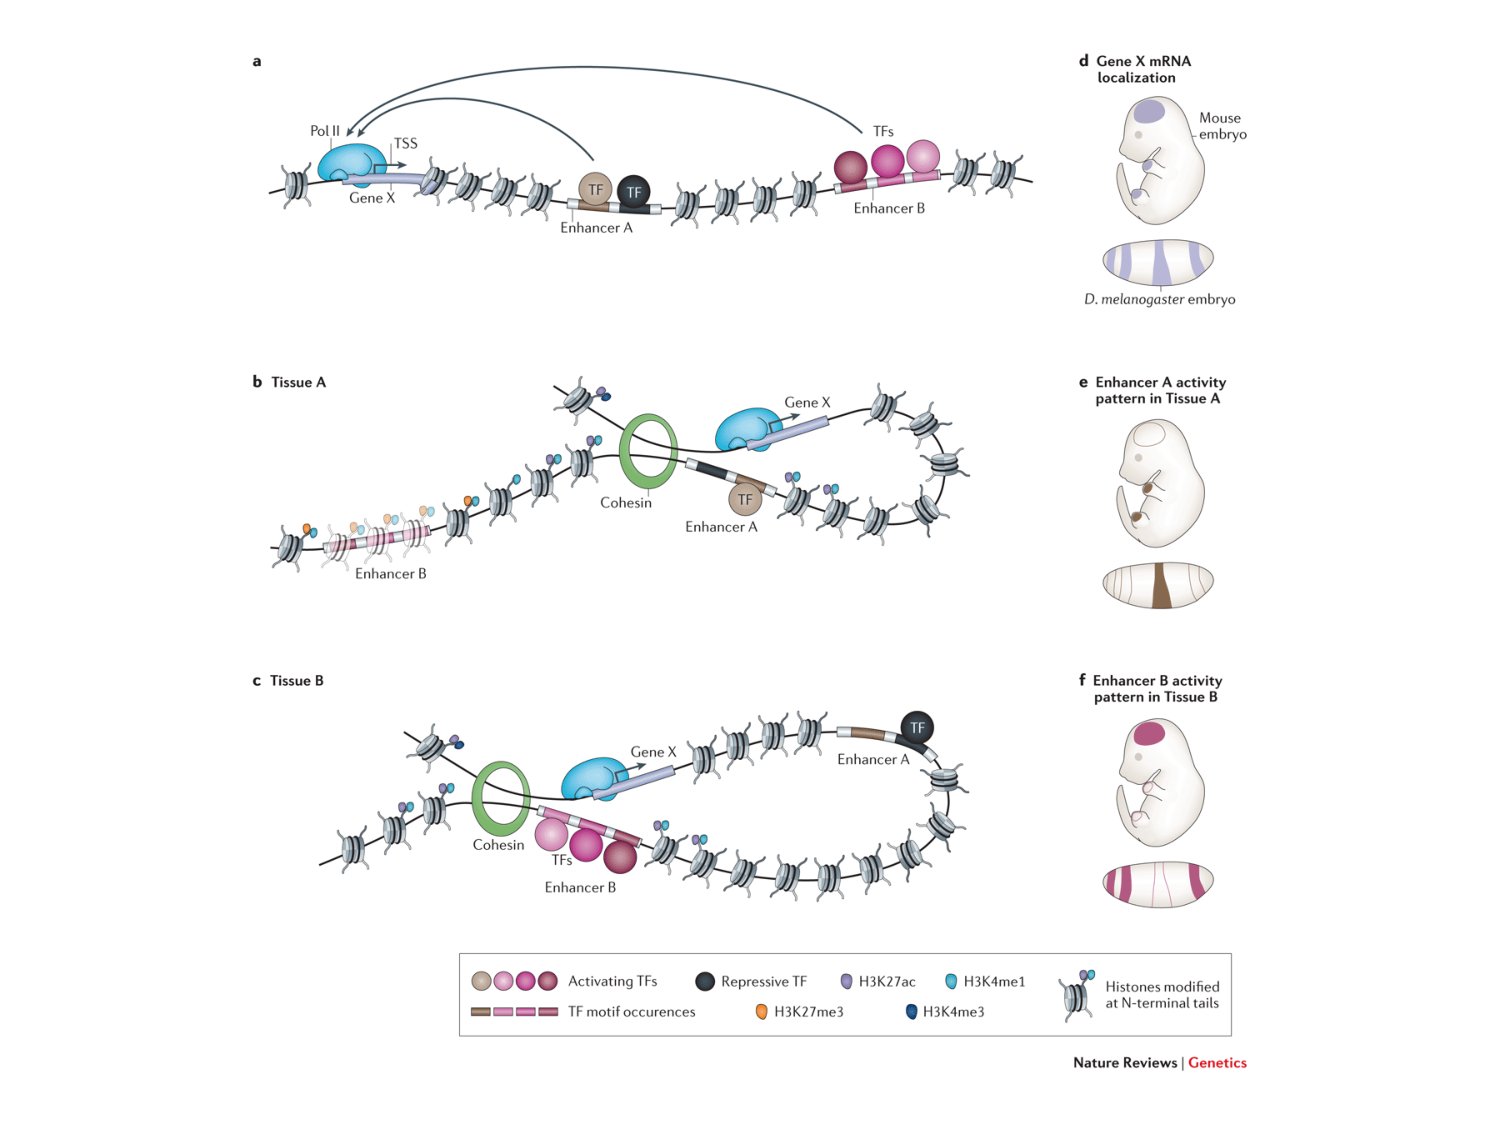
\includegraphics[width=0.8\linewidth]{intro/enhancer.pdf}{\tiny{\\Source: Daria Shlyueva, et al. Nature Reviews Genetics 15, 272–286 (2014)
doi:10.1038/nrg3682}}
\end{figure}
% a | Enhancers are distinct genomic regions (or the DNA sequences thereof) that contain binding site sequences for transcription factors (TFs) and that can upregulate (that is, enhance) the transcription of a target gene from its transcription start site (TSS). Along the linear genomic DNA sequence, enhancers can be located at any distance from their target genes, which makes their identification challenging. b,c | In a given tissue, active enhancers (Enhancer A in part b or Enhancer B in part c) are bound by activating TFs and are brought into proximity of their respective target promoters by looping, which is thought to be mediated by cohesin and other protein complexes. Moreover, active and inactive gene regulatory elements are marked by various biochemical features: active promoters and enhancers are characterized by a depletion of nucleosomes, which is the structural unit of eukaryotic chromatin. Nucleosomes that flank active enhancers show specific histone modifications, for example, histone H3 lysine 4 monomethylation (H3K4me1) and H3K27 acetylation (H3K27ac). Inactive enhancers might be silenced by different mechanisms, such as by the Polycomb protein-associated repressive H3K27me3 mark (part b) or by repressive TF binding (part c). d–f | Complex patterns of gene expression result from the additive action of different enhancers with cell-type- or tissue-specific activities. The schematic mouse and Drosophila melanogaster embryos are drawn after Refs 7,43. Pol II, RNA polymerase II.
\end{frame}

\begin{frame}[plain]%{Integrative analysis - histone modification}
\begin{figure}
 \centering
 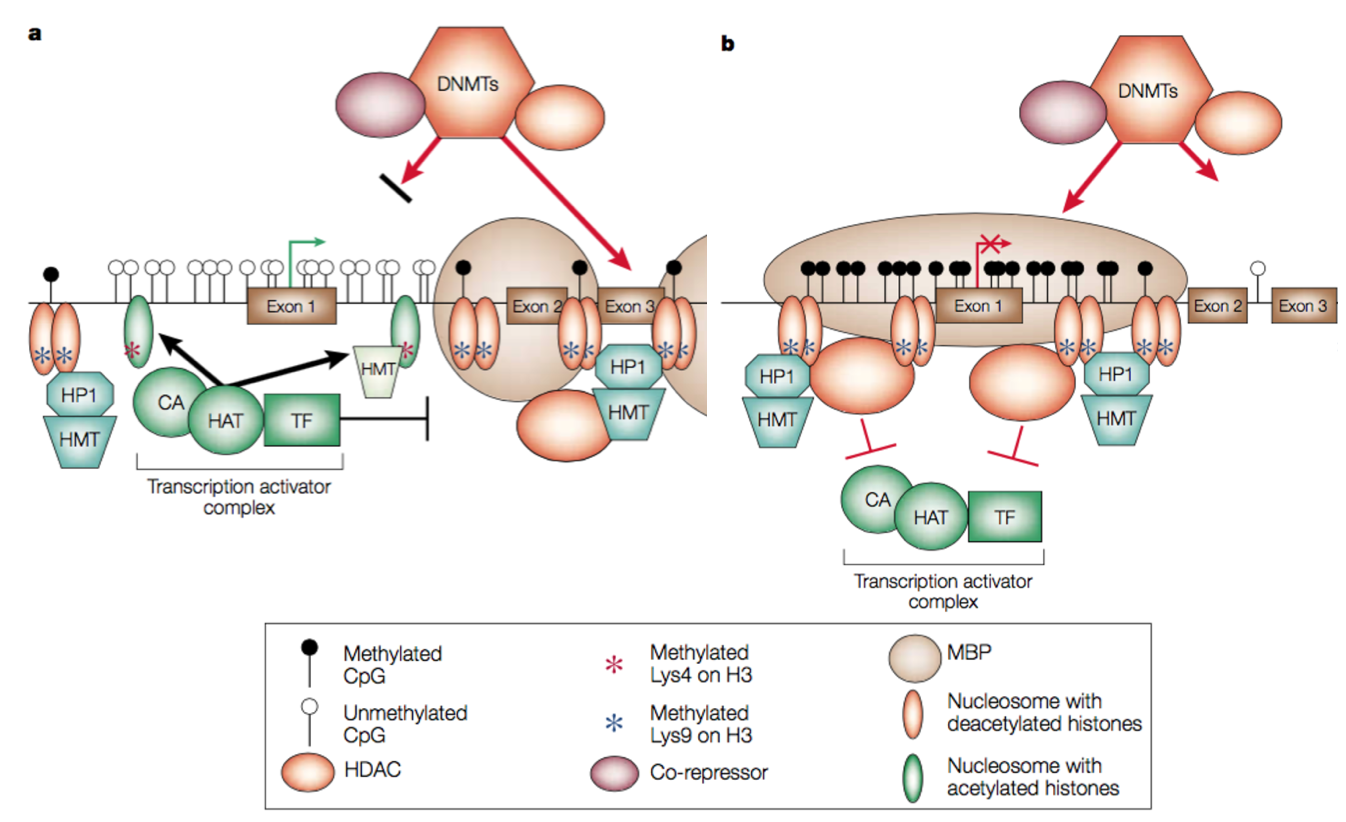
\includegraphics[width=1.05\linewidth]{images/DNAmethylation/5side2}{\tiny{\\Source: Peter A. Jones \& Stephen B. Baylin. Nature Reviews Genetics 3, 415–428 (2002) doi:10.1038/nrg816}}
\end{figure}
% a | Enhancers are distinct genomic regions (or the DNA sequences thereof) that contain binding site sequences for transcription factors (TFs) and that can upregulate (that is, enhance) the transcription of a target gene from its transcription start site (TSS). Along the linear genomic DNA sequence, enhancers can be located at any distance from their target genes, which makes their identification challenging. b,c | In a given tissue, active enhancers (Enhancer A in part b or Enhancer B in part c) are bound by activating TFs and are brought into proximity of their respective target promoters by looping, which is thought to be mediated by cohesin and other protein complexes. Moreover, active and inactive gene regulatory elements are marked by various biochemical features: active promoters and enhancers are characterized by a depletion of nucleosomes, which is the structural unit of eukaryotic chromatin. Nucleosomes that flank active enhancers show specific histone modifications, for example, histone H3 lysine 4 monomethylation (H3K4me1) and H3K27 acetylation (H3K27ac). Inactive enhancers might be silenced by different mechanisms, such as by the Polycomb protein-associated repressive H3K27me3 mark (part b) or by repressive TF binding (part c). d–f | Complex patterns of gene expression result from the additive action of different enhancers with cell-type- or tissue-specific activities. The schematic mouse and Drosophila melanogaster embryos are drawn after Refs 7,43. Pol II, RNA polymerase II.
\end{frame}

\begin{frame}{Databases - GDC}
\vspace*{-0.5cm}
\begin{figure}
 \centering
 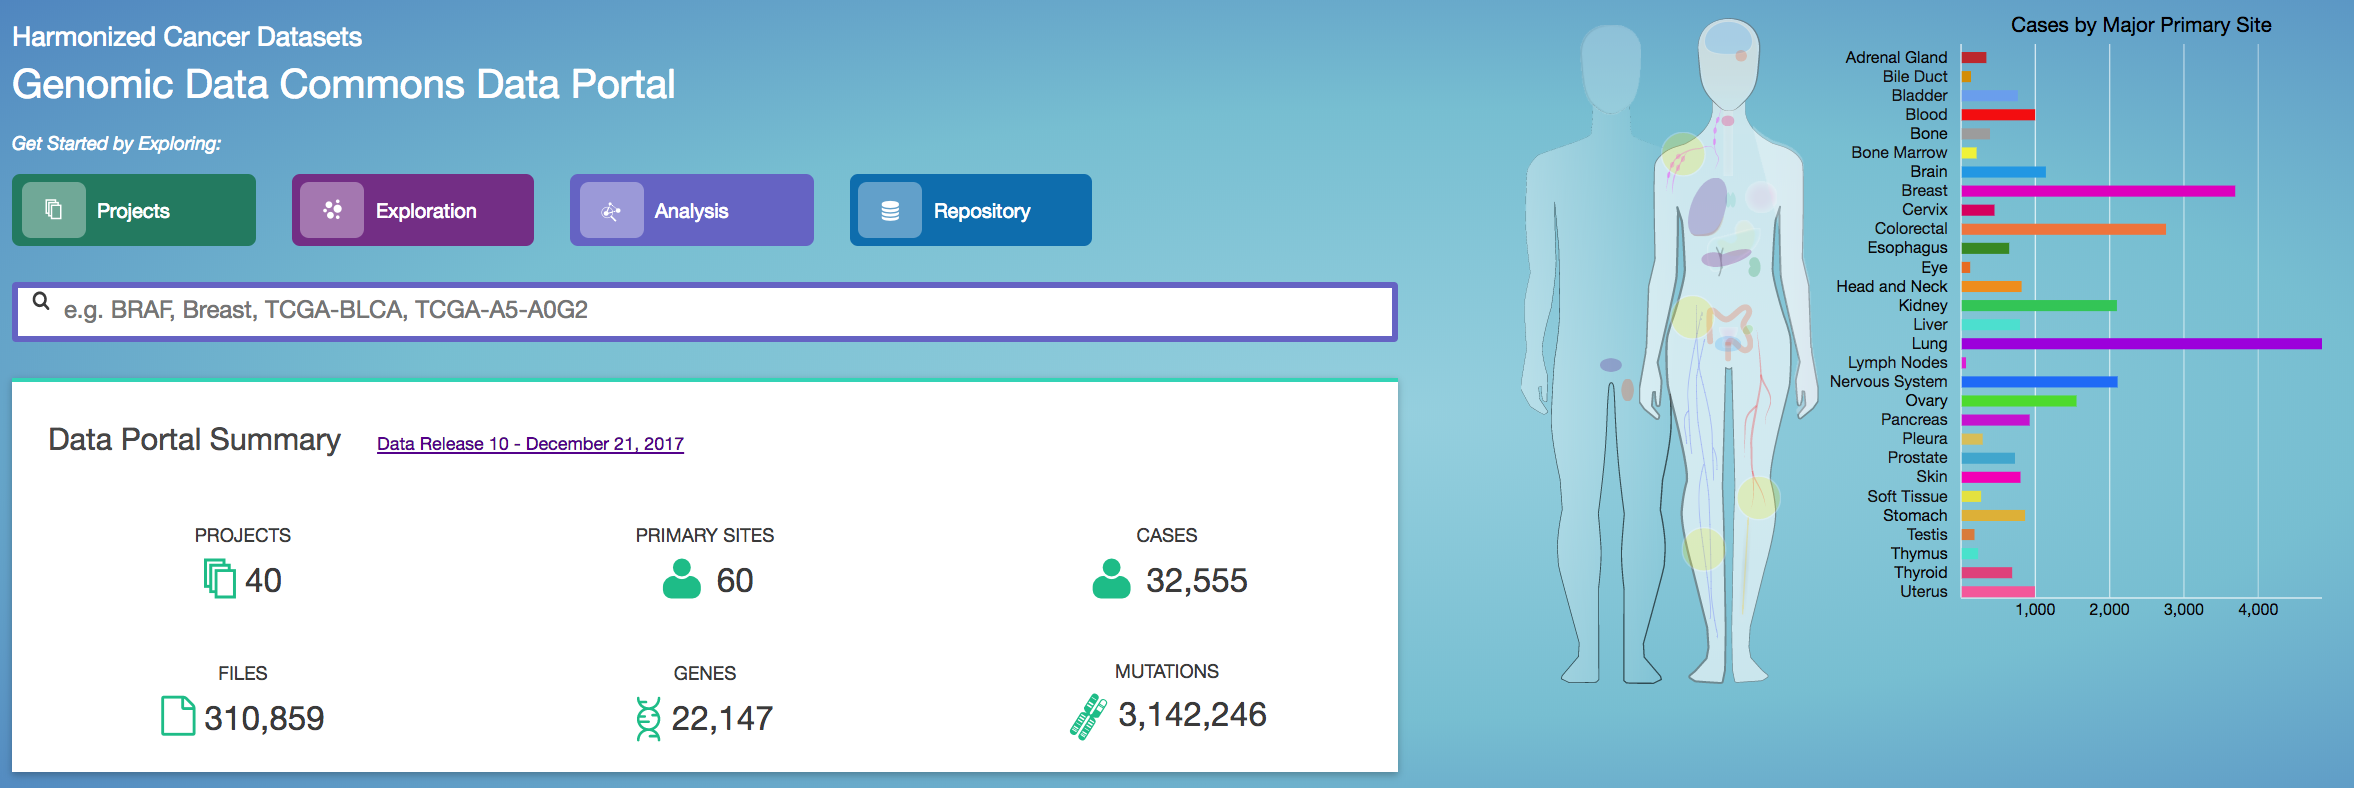
\includegraphics[width=1.0\linewidth]{intro/GDC.png}{\tiny{\\Source: The NCI's Genomic Data Commons (GDC), Accessed: 26-12-2017}}
\end{figure}
\end{frame}

\begin{frame}{Databases - ENCODE and ROADMAP}
\begin{figure}
 \centering
 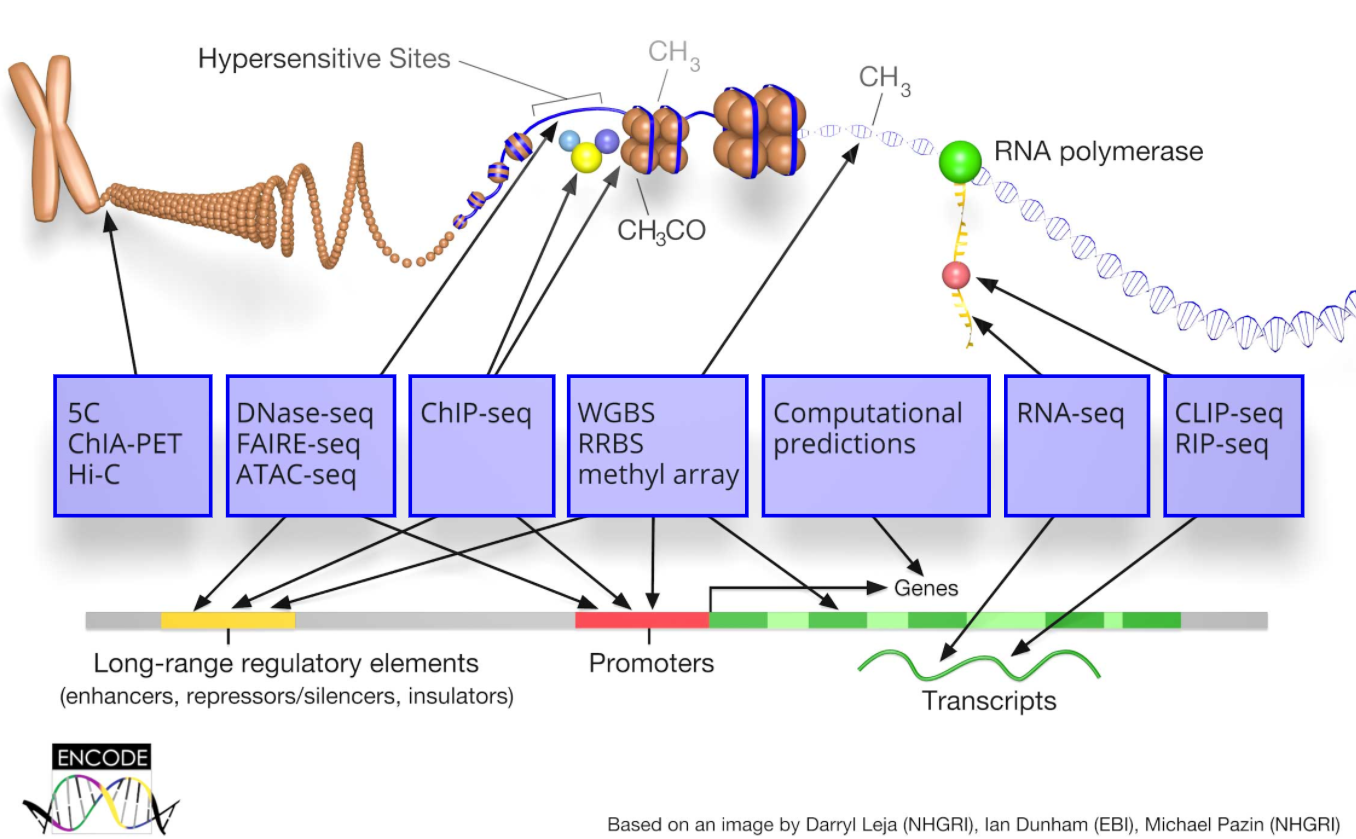
\includegraphics[width=0.7\linewidth]{intro/ENCODE.png}
 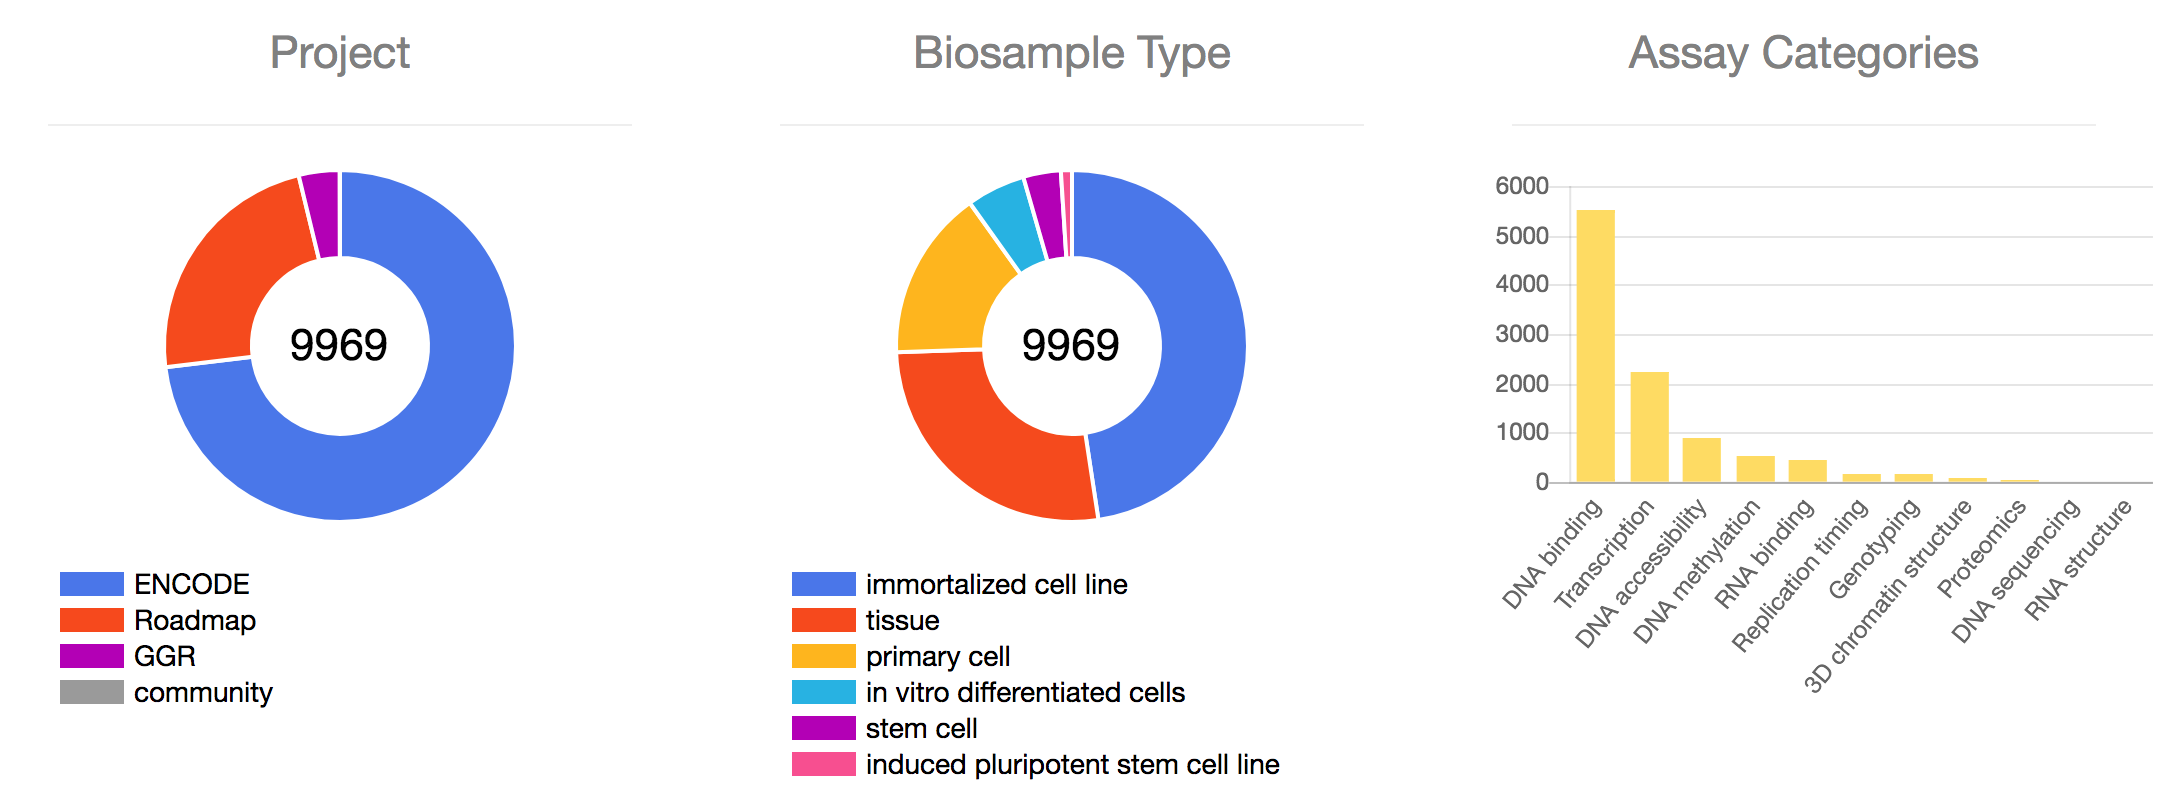
\includegraphics[width=0.7\linewidth]{intro/databases.png}{\tiny{\\Source:   (ENCODE: Encyclopedia of DNA Elements, Accessed: 26-12-2017}}
\end{figure}
\end{frame}

\begin{frame}{Integrative analysis}
 \vspace*{-0.5cm}
\begin{block}{Functional enrichment analysis of cancer signatures}
     A method to identify classes of genes or proteins that are over-represented in a large set of genes or proteins and may have an association with disease phenotypes. Example: GSEA.
\end{block}
\begin{figure}
 \centering
 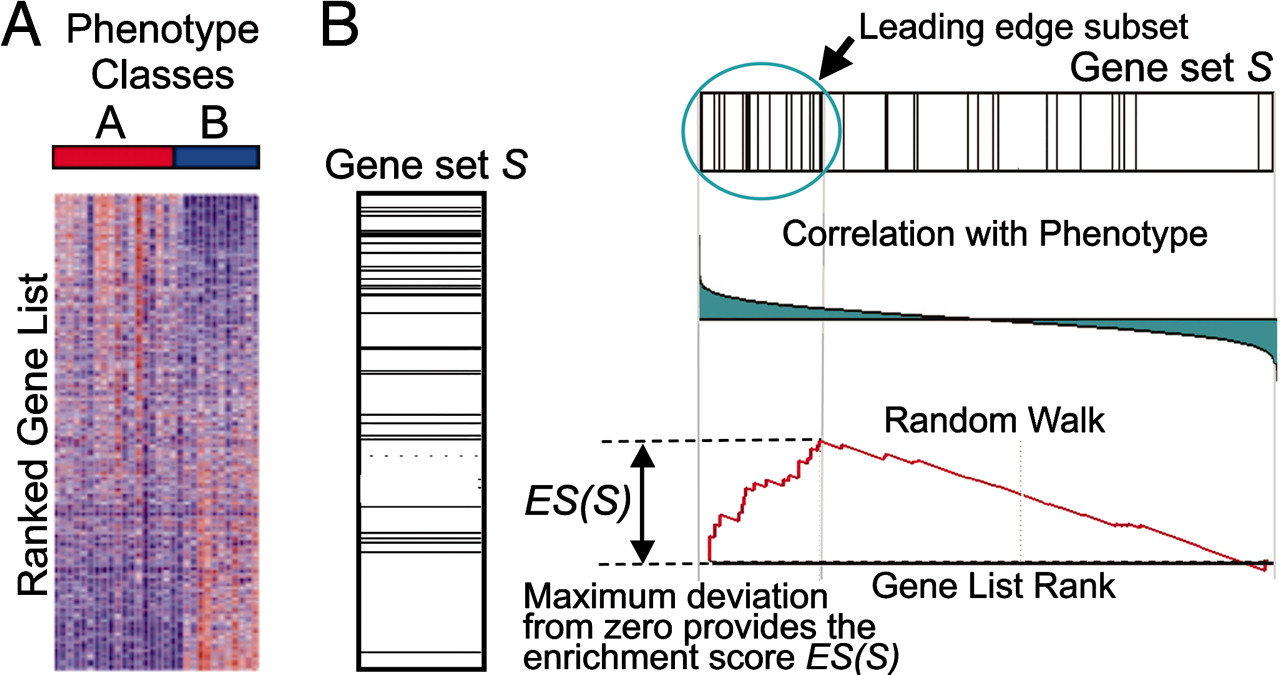
\includegraphics[width=0.7\linewidth]{intro/gsea.jpg}{\tiny{\\Source: Subramanian, Aravind, et al. DOI: 10.1073/pnas.0506580102.}}
\end{figure}

\end{frame}

%\begin{frame}{Integrative analysis}
% \vspace*{-0.2cm}
%\begin{block}{Protein interaction networks and cancer signatures}
%      Protein-protein interactions (PPIs) are essential to almost every process in a cell and are crucial for understanding %cell physiology in normal and disease states.
%\end{block}
%\begin{figure}
% \centering
% 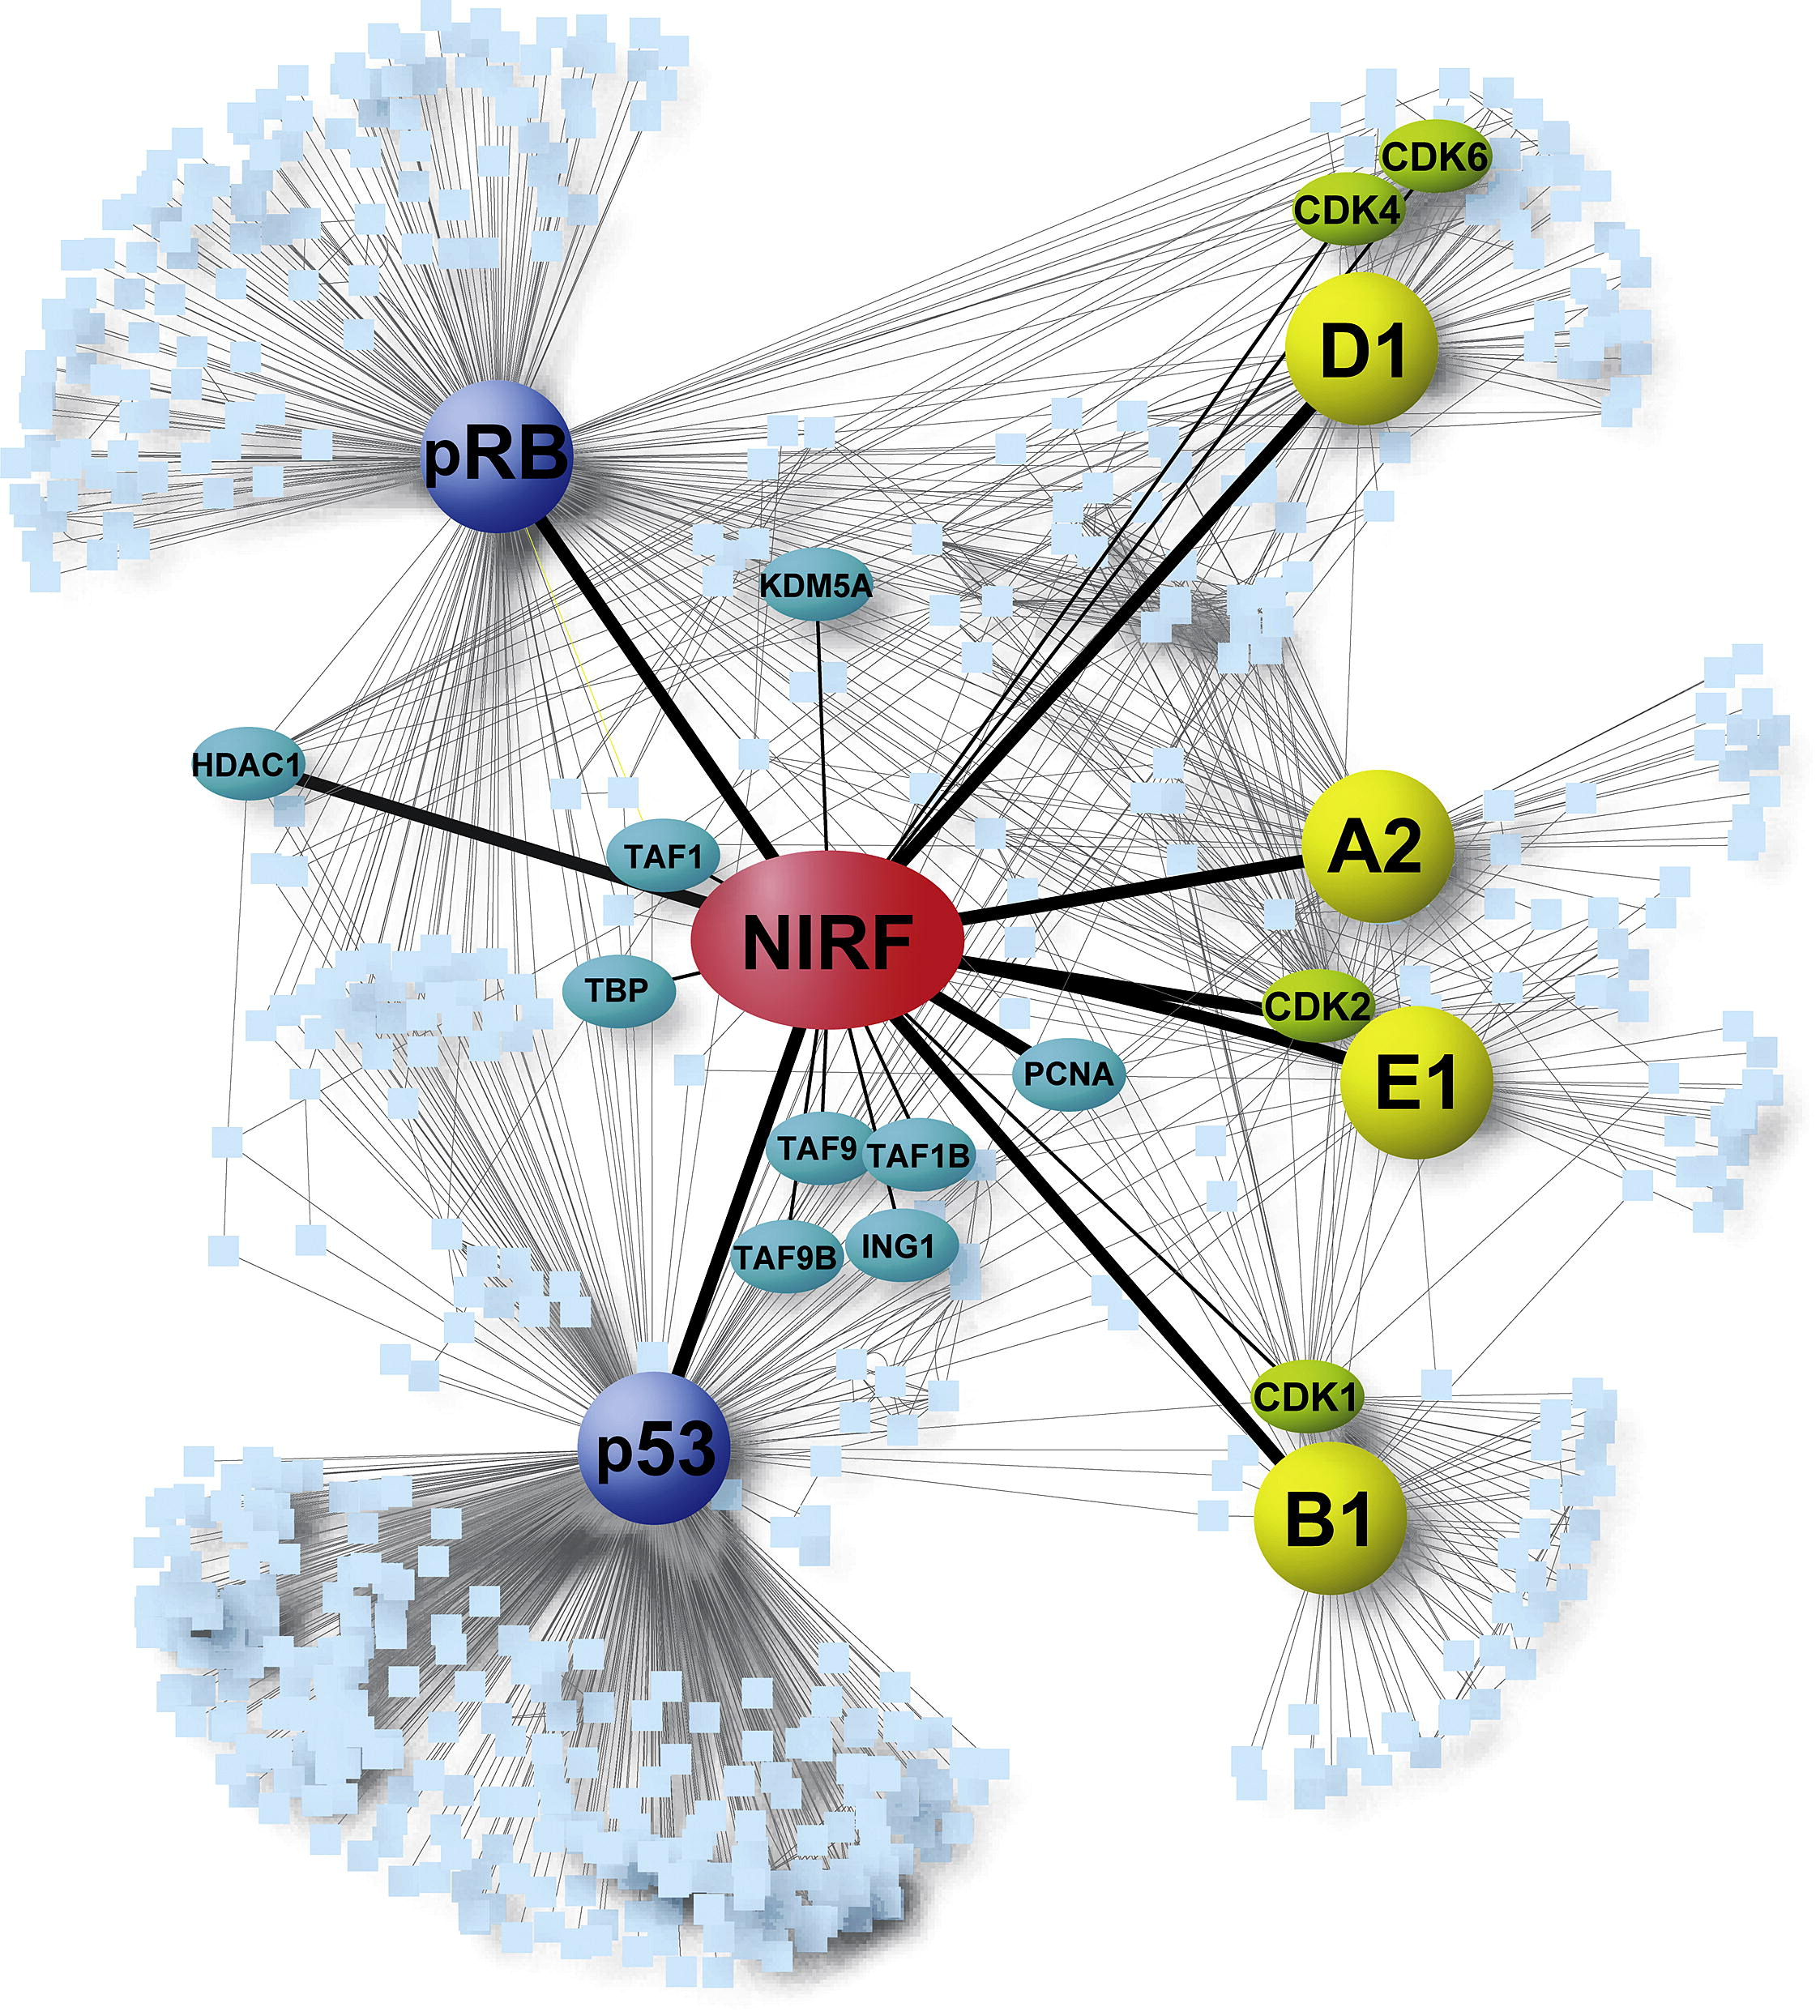
\includegraphics[width=0.35\linewidth]{intro/PPIN.jpg}{\tiny{\\Source: Mori, Tsutomu, et al. FEBS Letters 2012 https://doi.org/10.1016/j.febslet.2012.04.038}}
%\end{figure}
% Fig. 3. The NIRF protein–protein interaction network. NIRF interacts with the core cell cycle proteins (cyclin A2, cyclin B1, cyclin D1, cyclin E1, pRB, and p53) and other nuclear proteins. These core cell cycle proteins are hub proteins with many interacting partners, and thereby constitute individual network modules. NIRF is positioned at the center of these modules, thereby connecting the modules to one another. The symbols used are as follows: yellow, cyclins; yellow–green, CDKs; blue, two major tumor suppressors; green, NIRF-interacting proteins retrieved from a database [121]. The thicker black lines indicate interactions demonstrated by more than two methods. (Reproduced with permission from reference [3]).
%\end{frame}

\begin{frame}{Integrative analysis}
 \vspace*{-0.3cm}
\begin{block}{Global transcriptional networks}
If the targets of all transcription factors were known, then one could easily infer which transcription factors must be activated in a tumor to yield the observed cancer signature.
\end{block}
\begin{exampleblock}{ of transcription factor-binding sites (TFBSs)}
\begin{itemize}
     \item Identification using High throughput experimental methods (i.e. ChIP-sequencing)
     \item Prediction using in-silico sequence-based methods
\end{itemize}
\end{exampleblock}
\vspace*{-0.3cm}
\begin{figure}
 \centering
 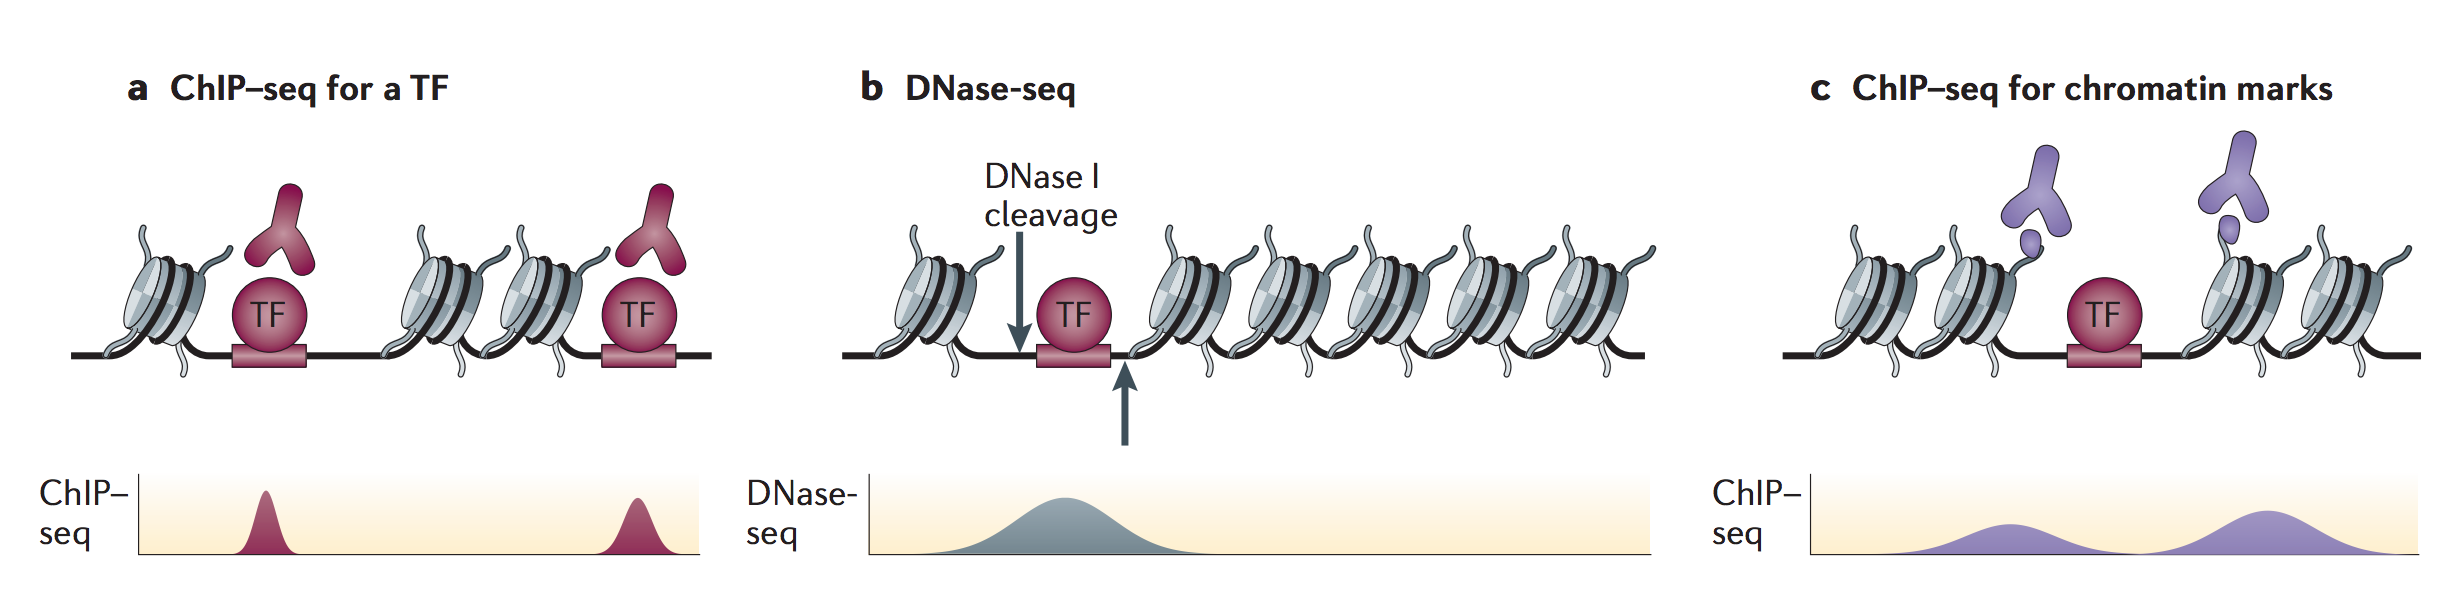
\includegraphics[width=1.0\linewidth]{intro/TF.png}{\tiny{\\Source: Daria Shlyueva, et al. Nature Reviews Genetics 15, 272–286 (2014) doi:10.1038/nrg3682}}
\end{figure}
% Fig. 3. The NIRF protein–protein interaction network. NIRF interacts with the core cell cycle proteins (cyclin A2, cyclin B1, cyclin D1, cyclin E1, pRB, and p53) and other nuclear proteins. These core cell cycle proteins are hub proteins with many interacting partners, and thereby constitute individual network modules. NIRF is positioned at the center of these modules, thereby connecting the modules to one another. The symbols used are as follows: yellow, cyclins; yellow–green, CDKs; blue, two major tumor suppressors; green, NIRF-interacting proteins retrieved from a database [121]. The thicker black lines indicate interactions demonstrated by more than two methods. (Reproduced with permission from reference [3]).
\end{frame}

\begin{frame}[plain]{TFBS prediction}
 \vspace*{-0.3cm}
\begin{figure}
 \centering
 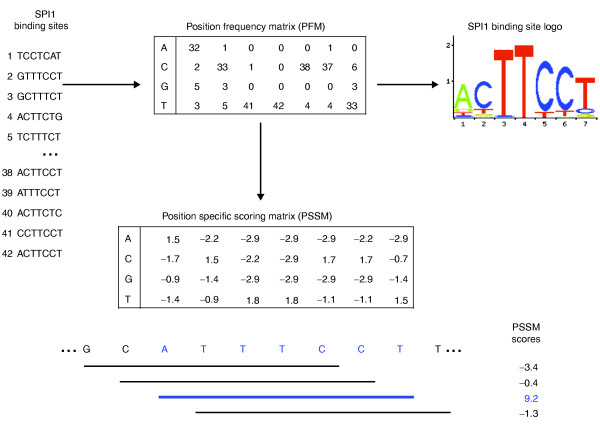
\includegraphics[width=0.95\linewidth]{intro/TFBS2.jpg}{\tiny{\\Source: Worsley-Hunt, R., et al.  Genome medicine. 2011 Oct 10;3(10):65. %Mathelier A, Wasserman WW. PLoS computational biology. 2013 Sep 5;9(9):e1003214.
 }}
\end{figure}
% https://www.nature.com/scitable/blog/bio2.0/your_friend_the_sequence_logo
% Transcription factor binding site (TFBS) motif model. Sequences known to be bound by a specific transcription factor (for example, SPI1) are aligned. A position frequency matrix (PFM) is generated by counting the number of times each type of nucleotide occurs at each position of the alignment. The PFM is then converted to a log-scale position-specific scoring matrix (PSSM). The score of any DNA sequence window, having the same length as the matrix, is calculated by summing the corresponding nucleotide values from the PSSM. The PFM may also be represented as a binding site logo, depicting the nucleotide properties of the TFBSs.
% The greater the height of the letter corresponding to a nucleotide, the higher the information content and higher the probability of getting it at this position.
% Figure 2. Sequence logo representing a TFFM.(A) Graphical representation of a TFFM constructed for the Hnf4A TF. Each column corresponds to a position within a TFBS. Each row captures the probabilities of each nucleotide to appear depending on the nucleotide found at the previous position. The opacity of a case represents the probability of hitting this case depending on the probability of appearance of the corresponding nucleotide at the previous position (the higher the opacity, the higher the probability). (B) The summary logo compacts all the information to summarize the dense logo in (A). (C) Zooming in on the dense TFFM logo for positions 10 to 13 (corresponding to the box in (A)). We observe that a “C” is more likely to appear at position 12 if nucleotide “T” was found at position 11 whereas a “T” is more likely to appear at position 12 if nucleotide “G” was found at position 11.
\end{frame}

\begin{frame}{Integrative analysis}
 \vspace*{-0.3cm}
\begin{block}{Protein interaction networks and cancer signatures}
      Protein-protein interactions (PPIs) are essential to almost every process in a cell and are crucial for understanding cell physiology in normal and disease states.
\end{block}
\begin{figure}
 \centering
 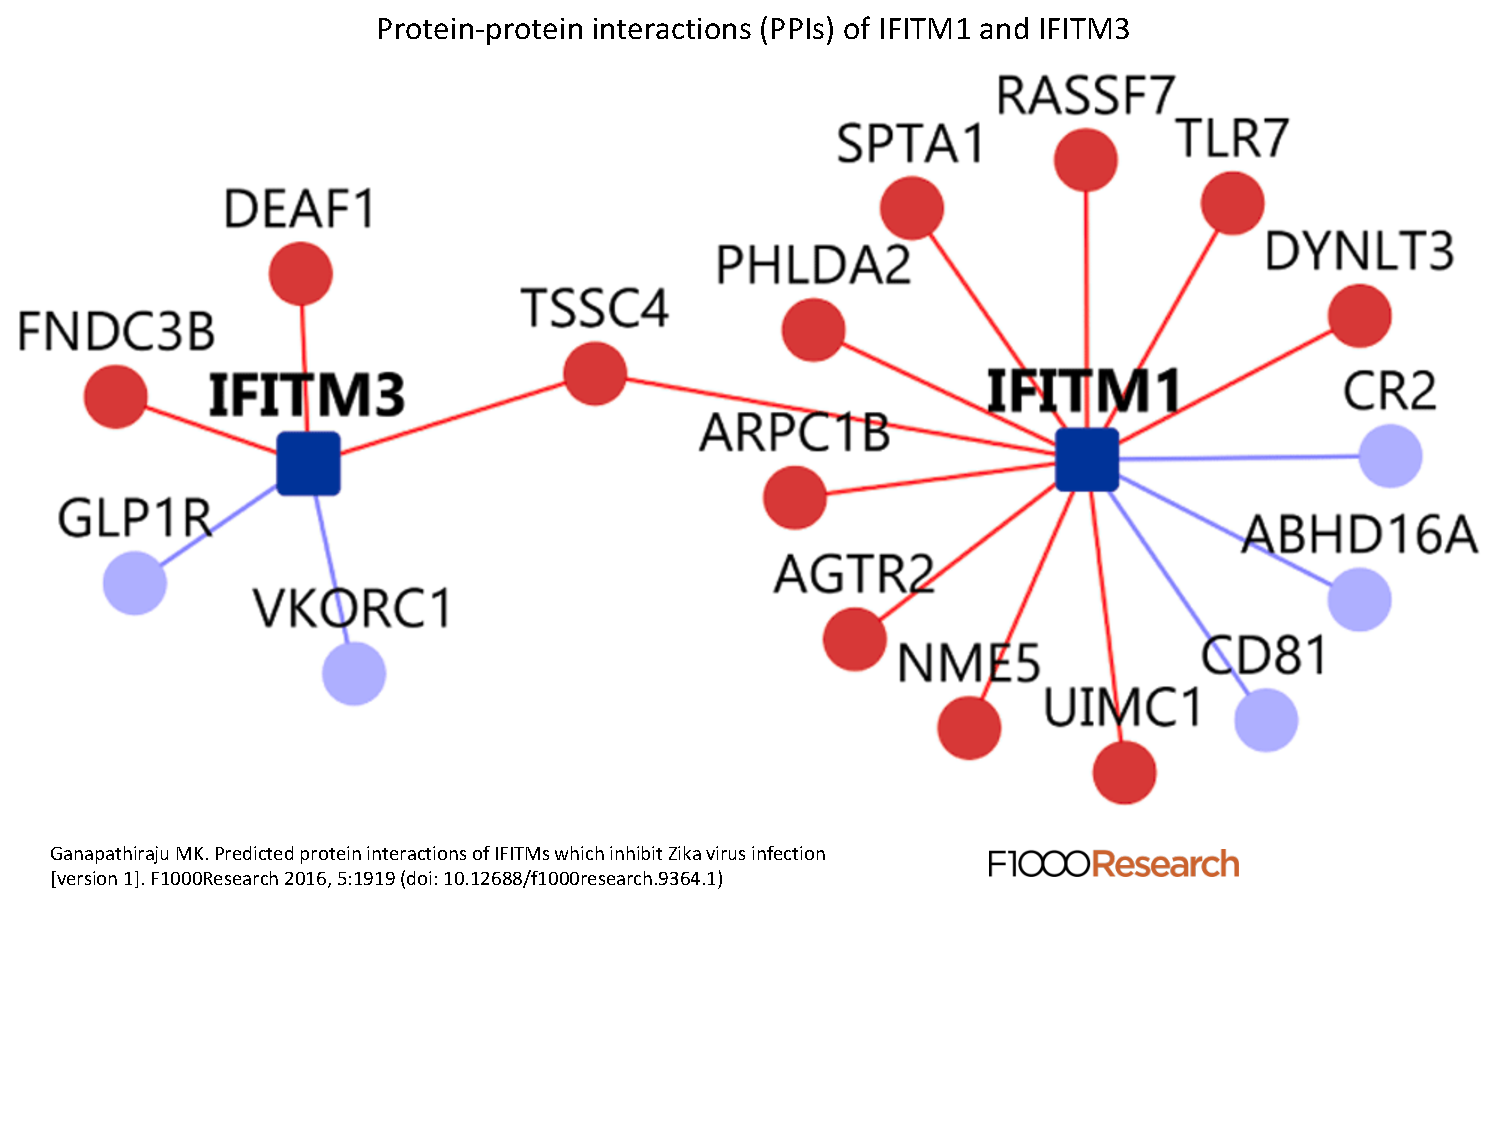
\includegraphics[width=0.8\linewidth]{intro/PPIN2.pdf}
\end{figure}
% Fig. 3. The NIRF protein–protein interaction network. NIRF interacts with the core cell cycle proteins (cyclin A2, cyclin B1, cyclin D1, cyclin E1, pRB, and p53) and other nuclear proteins. These core cell cycle proteins are hub proteins with many interacting partners, and thereby constitute individual network modules. NIRF is positioned at the center of these modules, thereby connecting the modules to one another. The symbols used are as follows: yellow, cyclins; yellow–green, CDKs; blue, two major tumor suppressors; green, NIRF-interacting proteins retrieved from a database [121]. The thicker black lines indicate interactions demonstrated by more than two methods. (Reproduced with permission from reference [3]).
\end{frame}

\begin{frame}{Integrative analysis}
 \vspace*{-0.3cm}
\begin{block}{Epigenome}
       Regulates gene expression by organizing the nuclear architecture of the chromosomes, restricting or facilitating transcription factor access to DNA, and preserving a memory of past transcriptional activities
\end{block}

\begin{table}[]
\centering
\scriptsize
\caption[Histone and epigenomic marks]{Core set of histone modification marks and other epigenomic marks}
\begin{tabular}{ll}
\toprule
 \textbf{Epigenomic marks}   & \textbf{Role} \\ \toprule
 Histone H3 lysine 4 trimethylation (H3K4me3)  & Promoter regions \\
 Histone H3 lysine 4 monomethylation (H3K4me1) & Enhancer regions  \\
 Histone H3 lysine 36 trimethylation (H3K36me3) & Transcribed regions  \\
 Histone H3 lysine 27 trimethylation (H3K27me3) & Polycomb repression  \\
 Histone H3 lysine 9 trimethylation (H3K9me3) & Heterochromatin regions \\
 Histone H3 acetylated at lysine 27 (H3K27ac)  &  Increase activation of genomic elements\\
 Histone H3 lysine 9 acetylation  (H3K9ac)  & Transcriptional activation \\
 DNase hypersensitivity &  Regions of accessible chromatin \\
 DNA methylation & Repressed regulatory regions\\  \bottomrule
\end{tabular}
\end{table}
\end{frame}

\begin{frame}[plain]%{Integrative analysis - histone modification}
 \vspace*{-0.3cm}
\begin{figure}
 \centering
 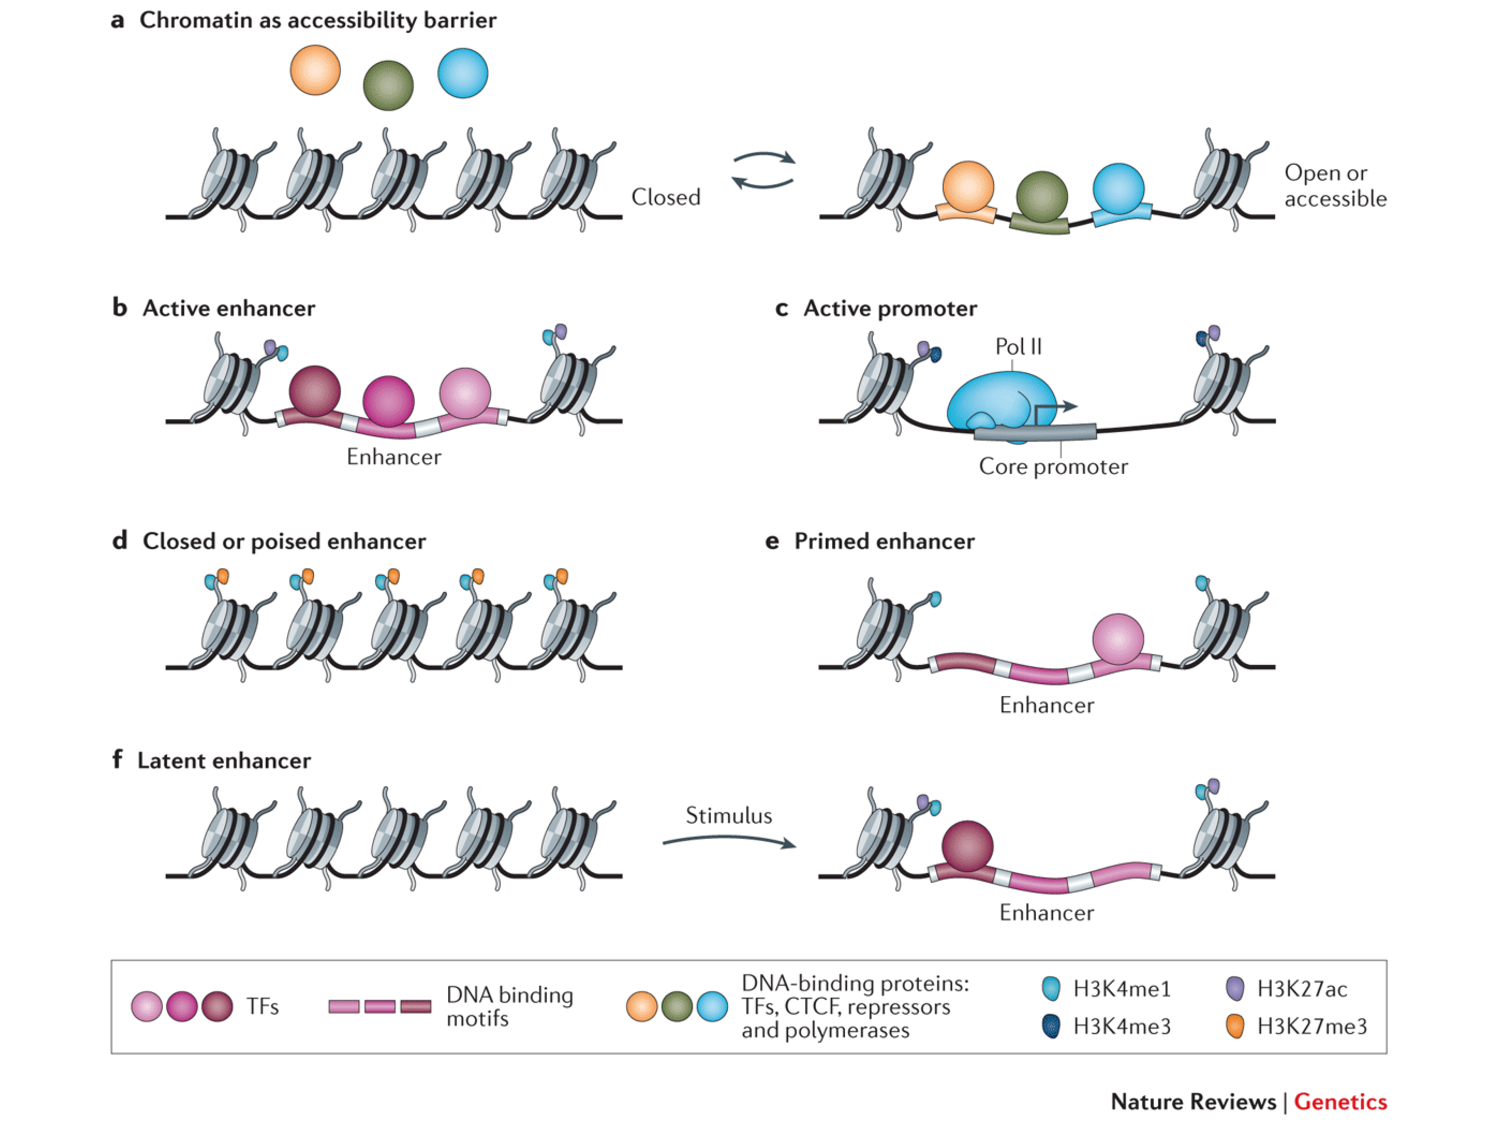
\includegraphics[width=1.05\linewidth]{intro/marks.pdf}{\tiny{\\Source: Daria Shlyueva, et al. Nature Reviews Genetics 15, 272–286 (2014) doi:10.1038/nrg3682}}
\end{figure}
% a | Enhancers are distinct genomic regions (or the DNA sequences thereof) that contain binding site sequences for transcription factors (TFs) and that can upregulate (that is, enhance) the transcription of a target gene from its transcription start site (TSS). Along the linear genomic DNA sequence, enhancers can be located at any distance from their target genes, which makes their identification challenging. b,c | In a given tissue, active enhancers (Enhancer A in part b or Enhancer B in part c) are bound by activating TFs and are brought into proximity of their respective target promoters by looping, which is thought to be mediated by cohesin and other protein complexes. Moreover, active and inactive gene regulatory elements are marked by various biochemical features: active promoters and enhancers are characterized by a depletion of nucleosomes, which is the structural unit of eukaryotic chromatin. Nucleosomes that flank active enhancers show specific histone modifications, for example, histone H3 lysine 4 monomethylation (H3K4me1) and H3K27 acetylation (H3K27ac). Inactive enhancers might be silenced by different mechanisms, such as by the Polycomb protein-associated repressive H3K27me3 mark (part b) or by repressive TF binding (part c). d–f | Complex patterns of gene expression result from the additive action of different enhancers with cell-type- or tissue-specific activities. The schematic mouse and Drosophila melanogaster embryos are drawn after Refs 7,43. Pol II, RNA polymerase II.
\end{frame}


\begin{frame}[plain]%{Integrative analysis - histone modification}
\vspace*{-0.5cm}
\begin{figure}
 \centering
 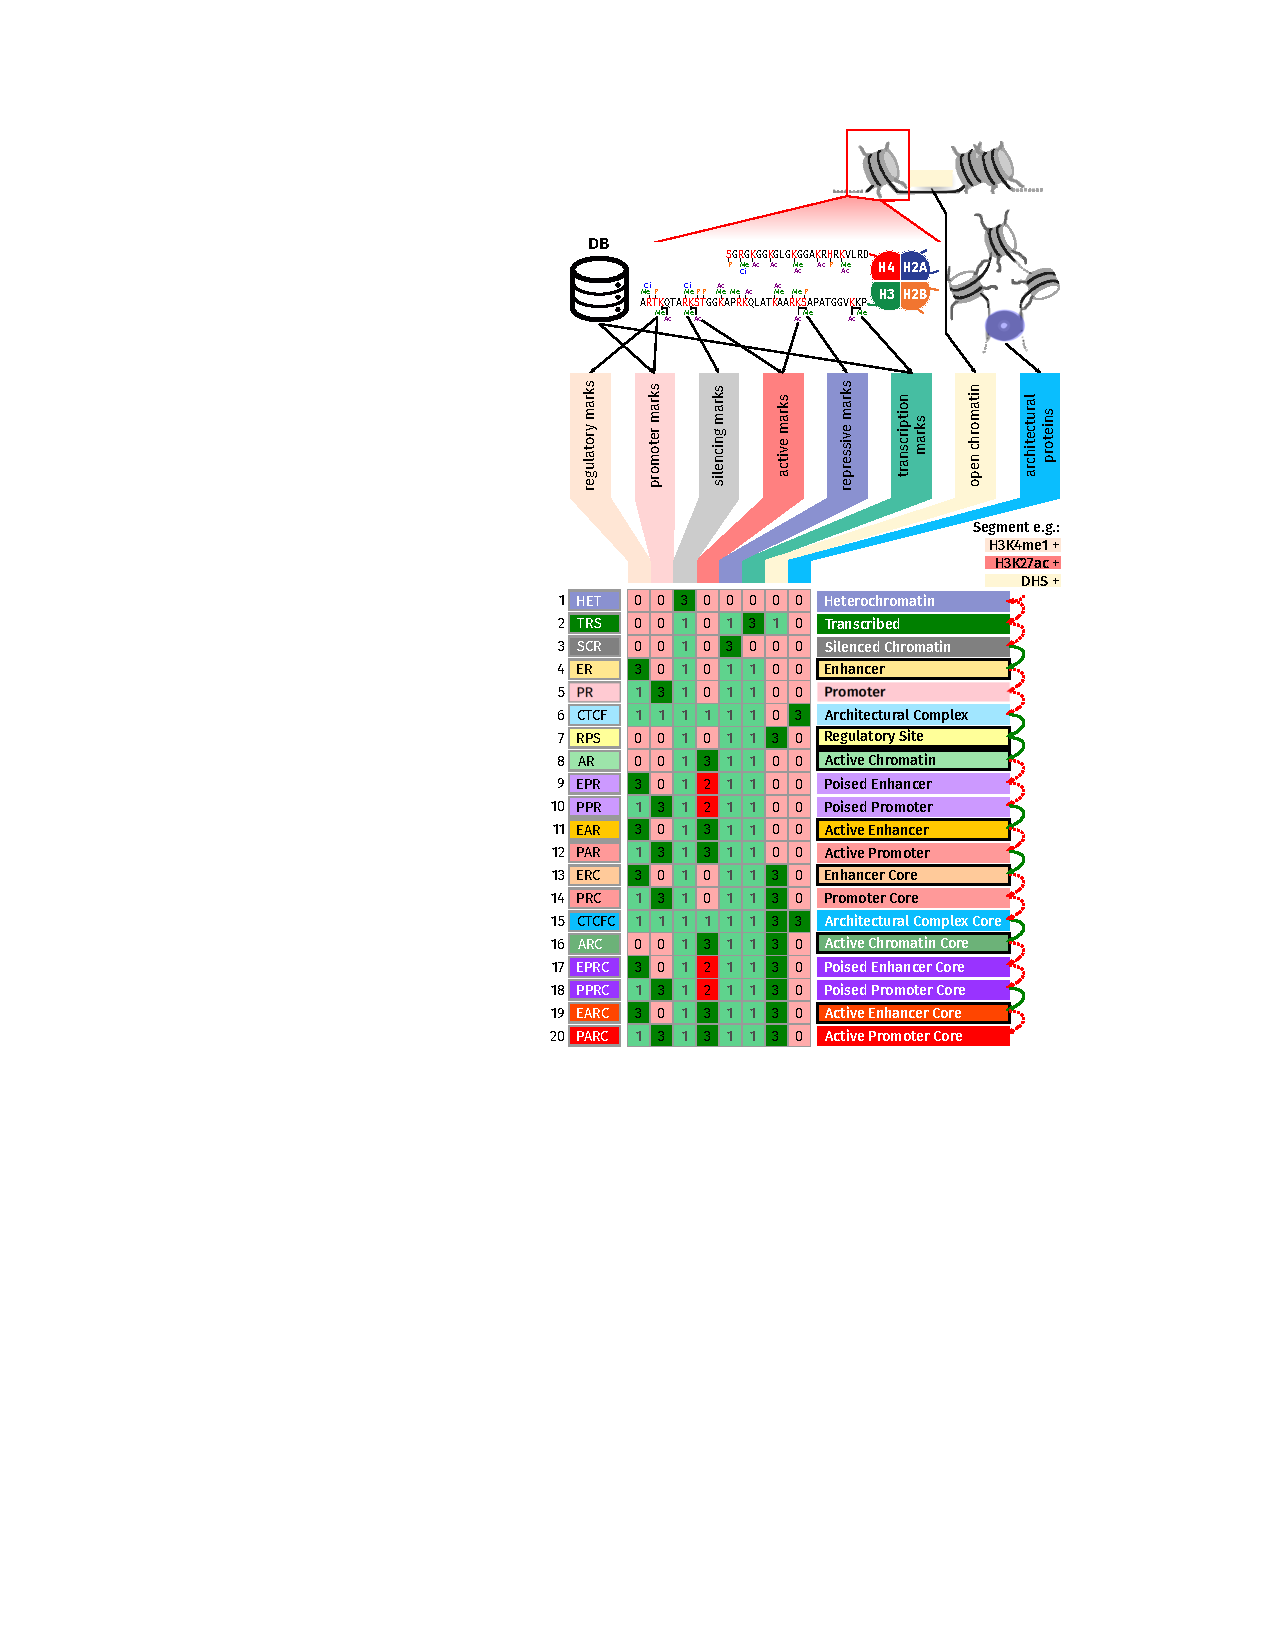
\includegraphics[width=0.5\linewidth]{intro/states.pdf}{\tiny{\\Source: Coetzee, Simon G., et al. "StateHub-StatePaintR: rapid and reproducible chromatin state evaluation for custom genome."}}
\end{figure}
\end{frame}
%a Figure 1. Mapping datasets to functional significance annotations. Experimental
% data and external database annotations are combined into abstraction layers
% (columns), integrated to produce chromatin states (rows) from the decision matrix.
% StatePaintR produces state assignments by iteratively comparing the marks that are
% present in each segment with each row of data in the table. The values of color-coded
% squares signify relationship between data and state: 0 (light red) the feature/data type
% negates the state but is not required to be present, 1 (light green) feature is consistent
% with the state but not required, 2 (red) if the feature is required to be available
% and negates the state, and 3 (green) it is both required and consistent with the state.
% Information content (sum of row values) of states increases from top to bottom. For
% the example, red dotted arrows indicate non-matching rows, and green arrows indicate
% matching rows. The state call corresponds to the last matched row


\section{Objectives}

\begin{frame}
\begin{alertblock}{Problem}
\begin{itemize}
\item Data is spread accross different databases and stored in different formats
\item Lack of computational tools and methods that can integrate and interpret such information
\end{itemize}
\end{alertblock}
\begin{exampleblock}{Steps performed manually by the user}
\begin{enumerate}
\item Access all databases
\item Select and process the data necessary to the project
\item Integrate that data using multiple downstream analysis tools to extract
\item Interpret the relevant biological information
\end{enumerate}
\end{exampleblock}
\end{frame}


\begin{frame}
\begin{block}{Main goals}
\begin{itemize}
\item Develop tools for searching, retrieving and analyzing pan-cancer genomic data from several databases (GDC, ENCODE, ROADMAP)
  \item Investigate the intergenic epigenomic changes associated with distinct biological and clinical subgroups of gliomas first discovered by our laboratory

\end{itemize}

\end{block}

\begin{block}{Secondary goals}
\begin{itemize}
  \item Use standard data structure to organize the data and the metadata
  \item Publish tools the open-source Bioconductor environment.
  \item Use learning machine algorithms for classifying an independent set of gliomas based on newly identified regulatory networks as related to pan-cancer deregulation;
\end{itemize}

\end{block}


\end{frame}

\begin{frame}[plain]{Tools}
\vspace*{-0.4cm}
\begin{figure}
 \centering
 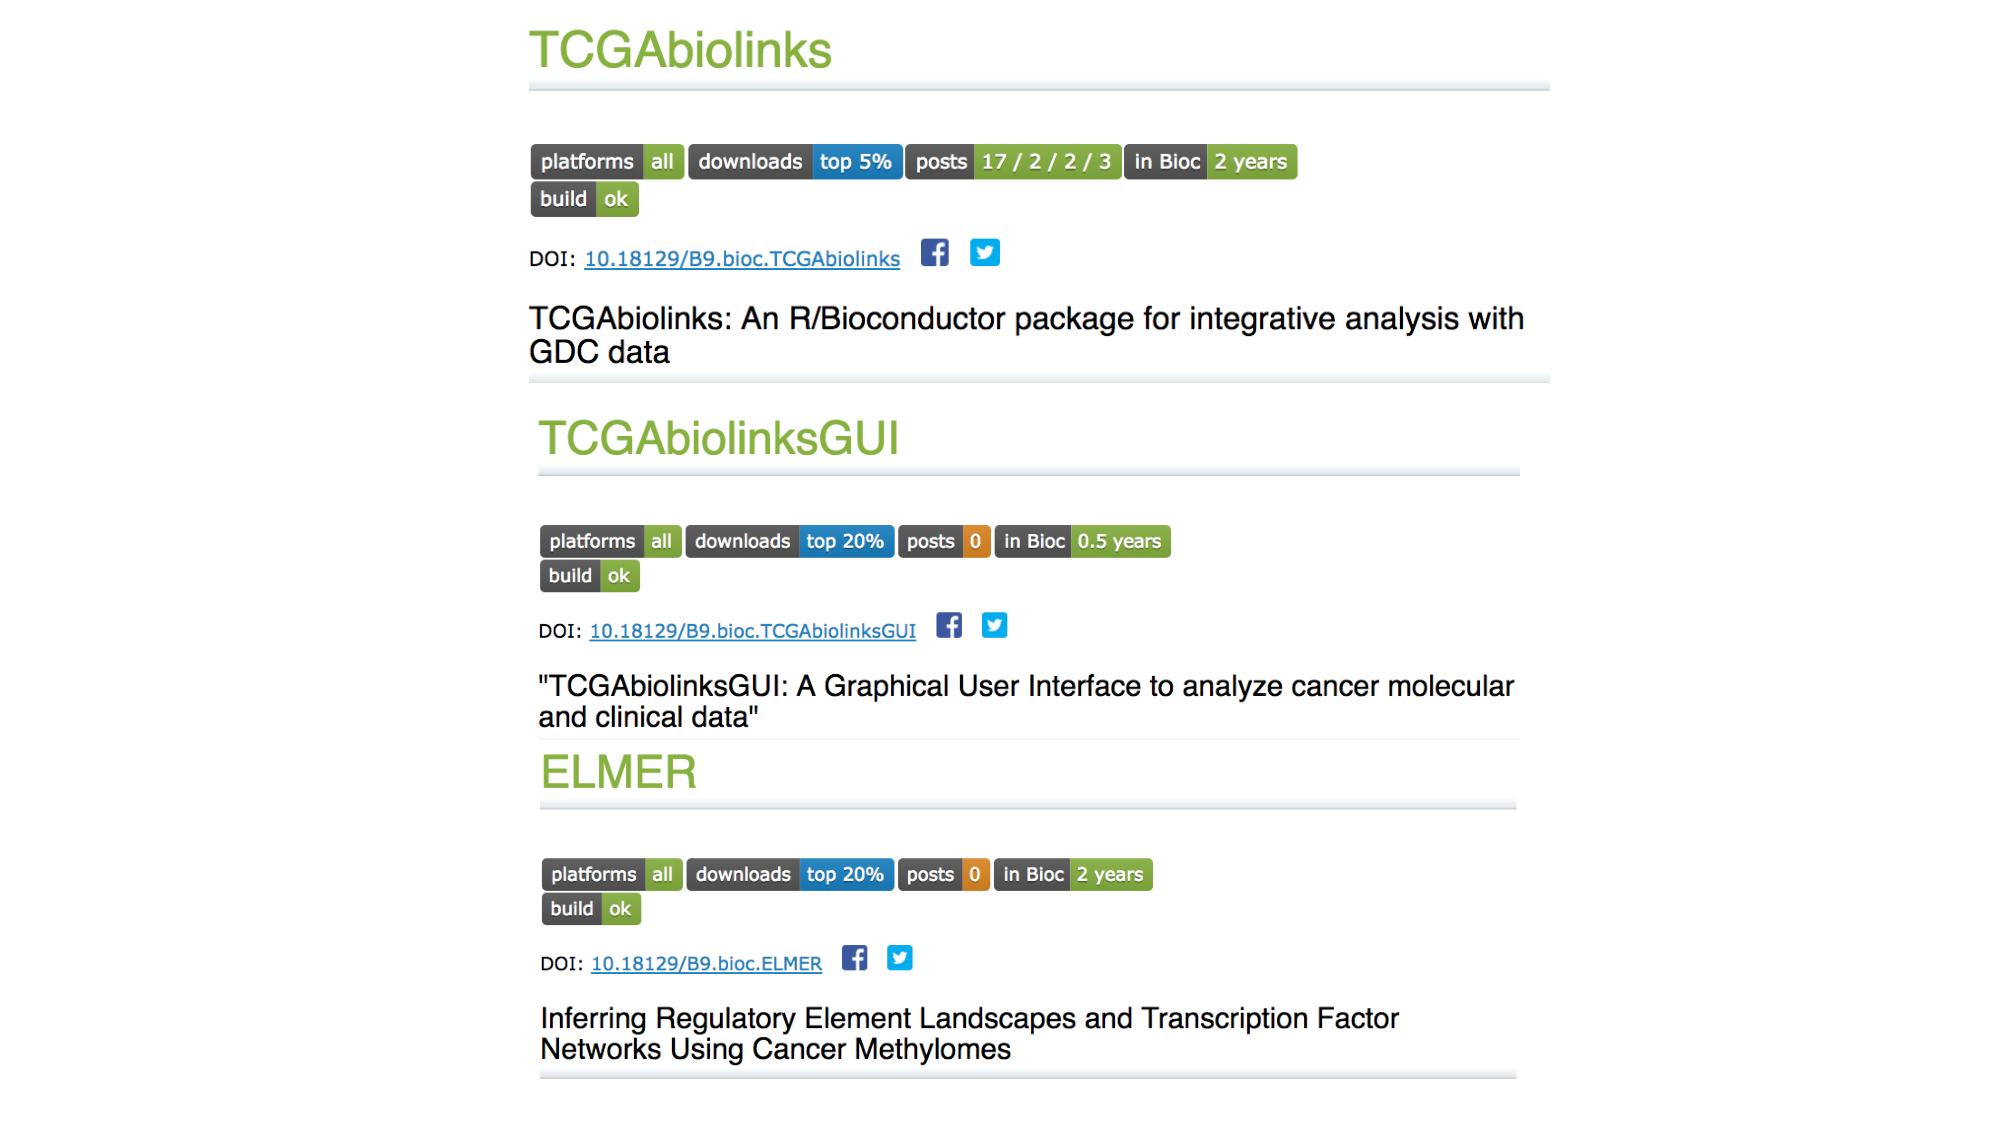
\includegraphics[width=0.75\linewidth]{intro/tools.pdf}
\end{figure}
\end{frame}

\section{TCGAbiolinks}

\begin{frame}{TCGAbiolinks functions}
 \begin{figure}
  \centering
  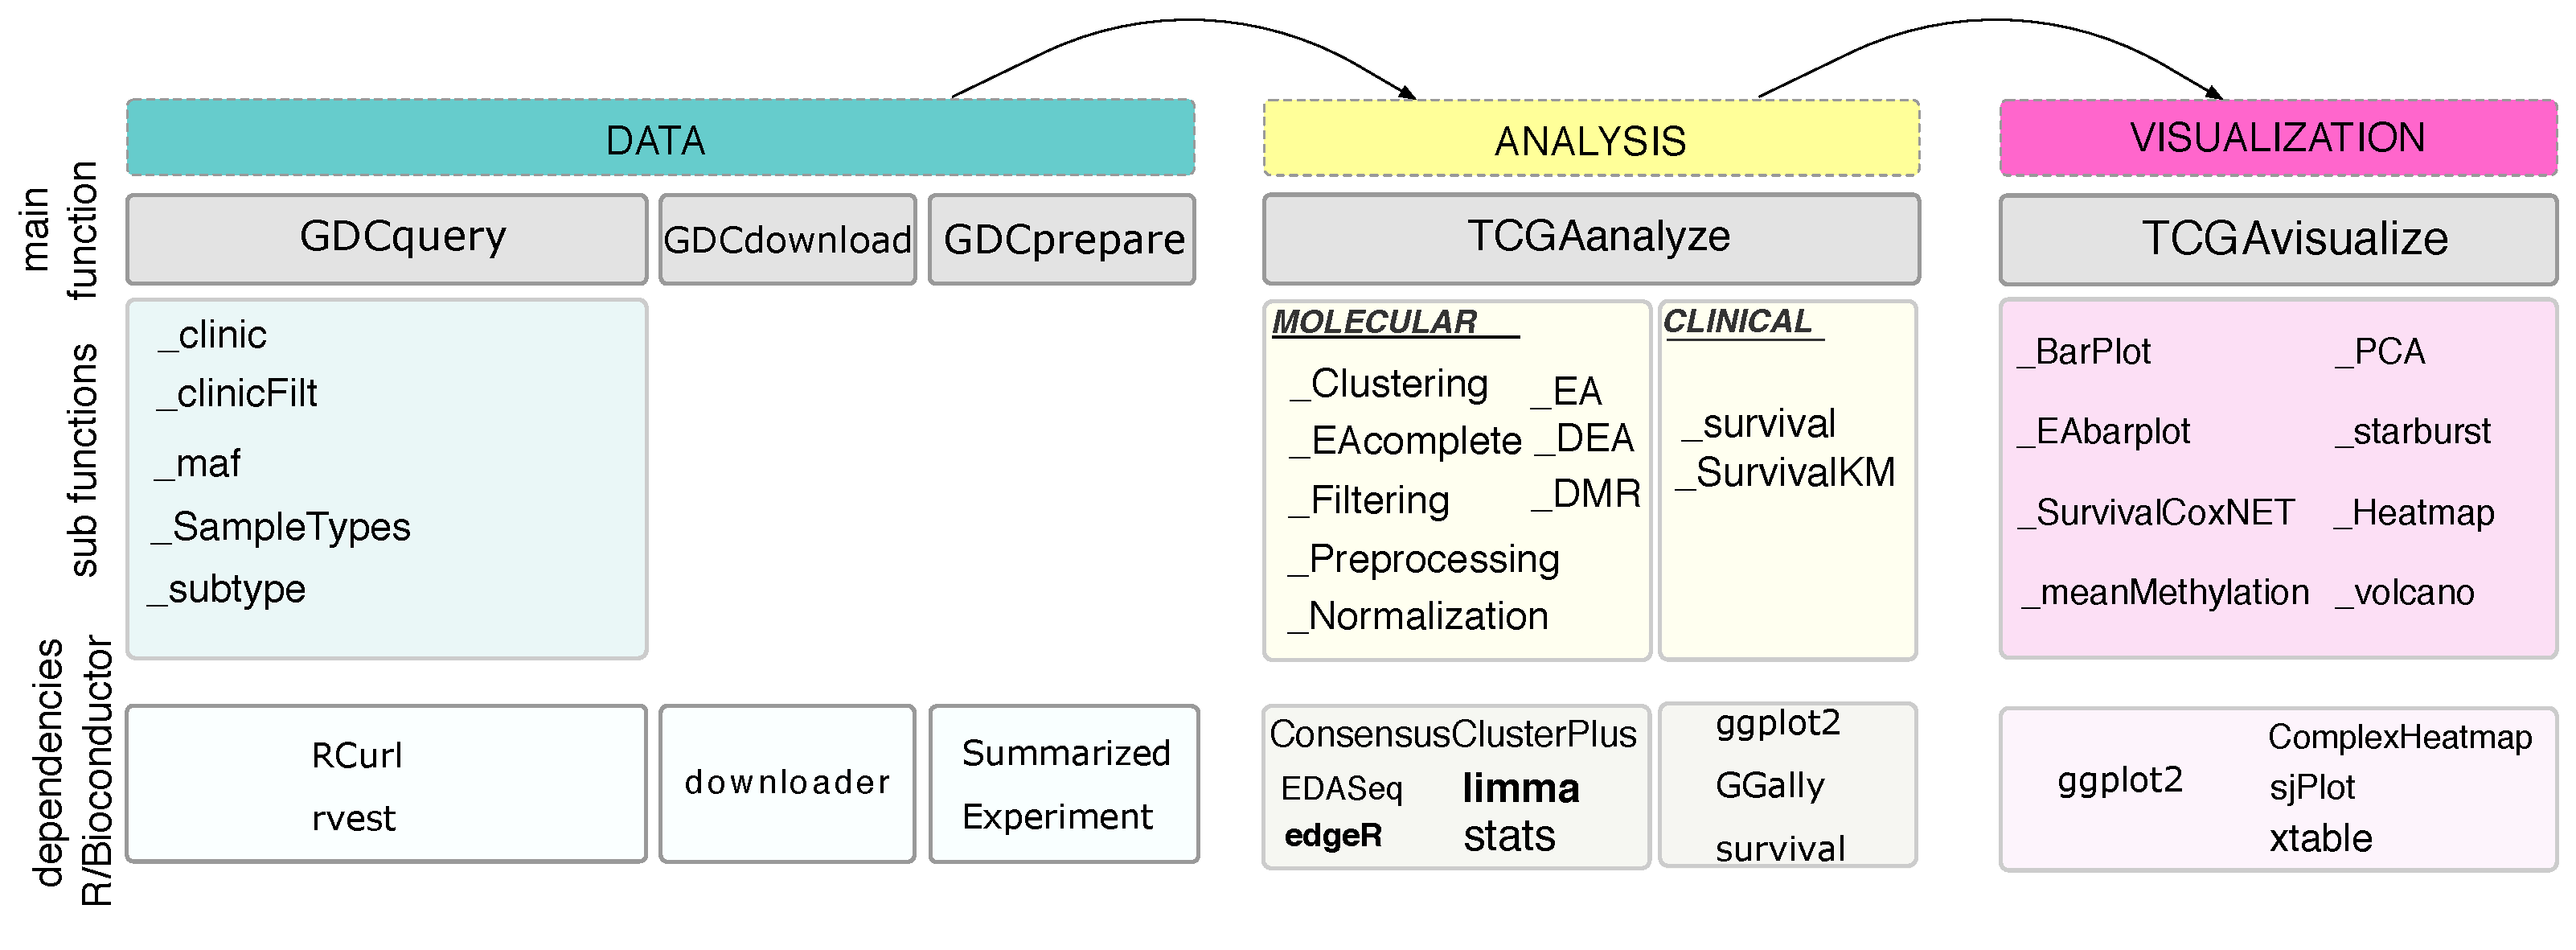
\includegraphics[width=1.0\linewidth]{TCGAbiolinks/summary.pdf}
  \caption{Overview of TCGAbiolinks functions}
 \end{figure}
\end{frame}

\begin{frame}{Data structure: SummarizedExperiment  }
 \vspace*{-0.5cm}
 \begin{figure}
  \centering
  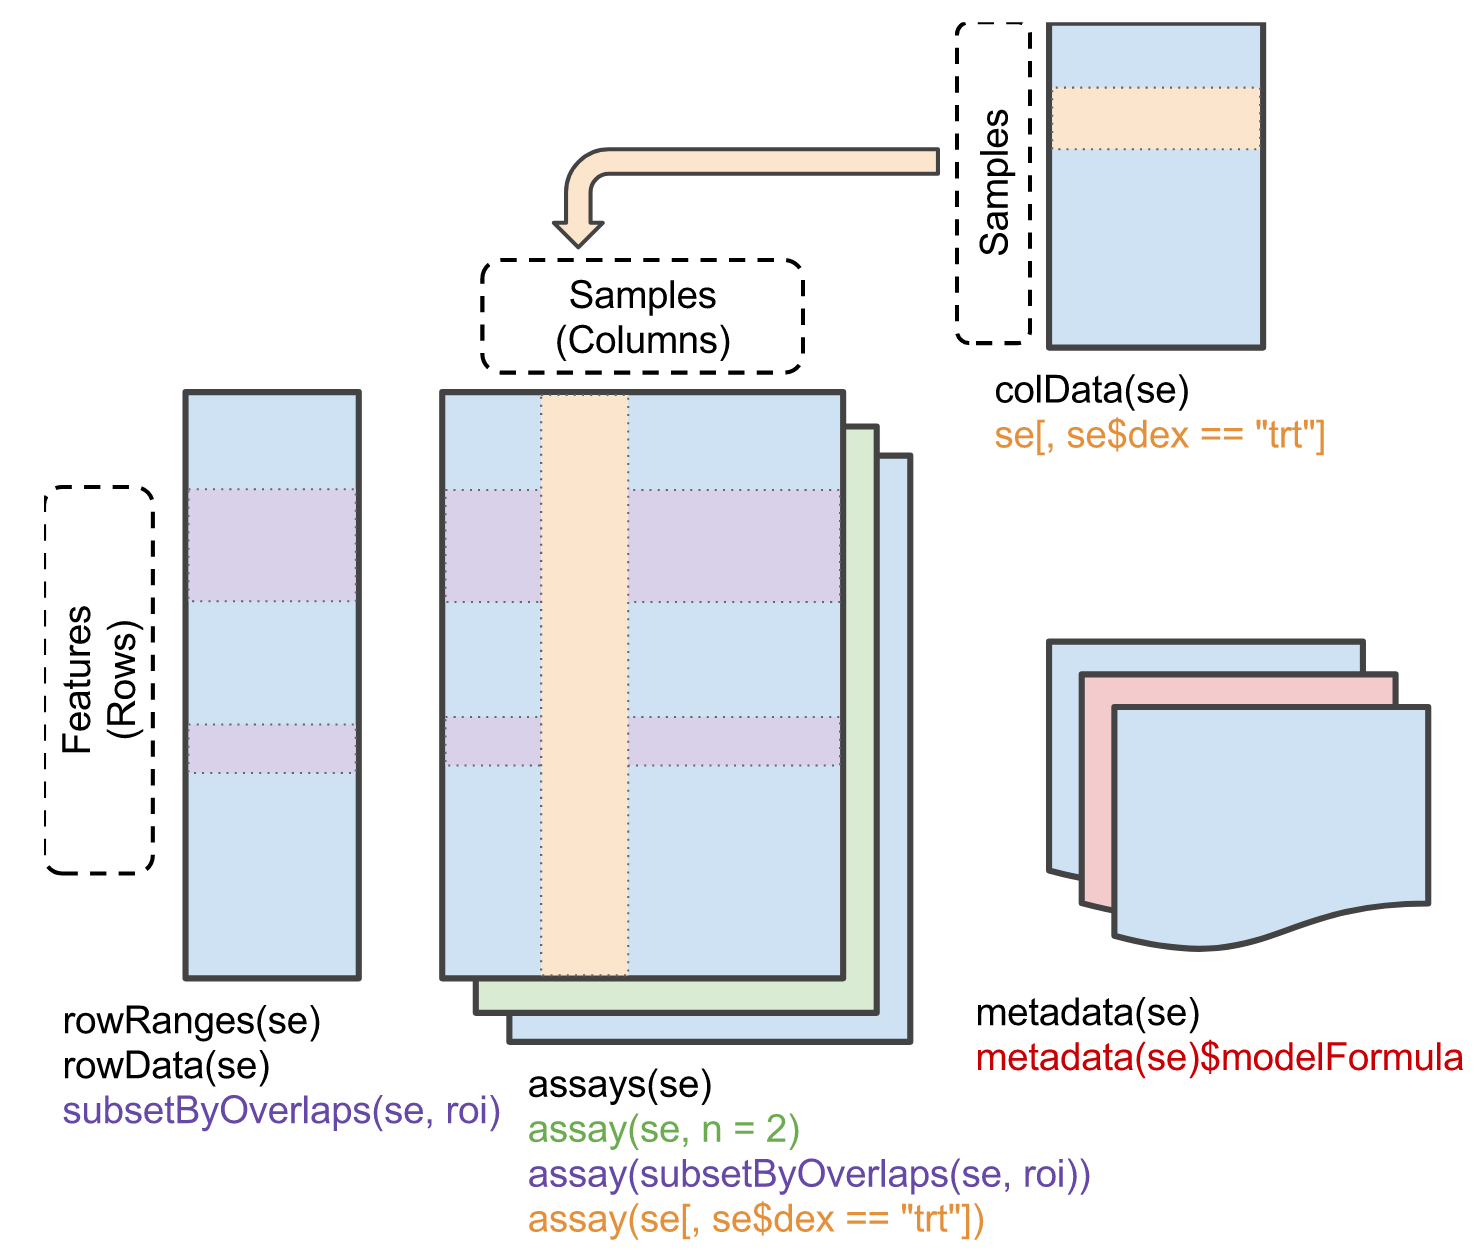
\includegraphics[width=0.7\linewidth]{TCGAbiolinks/summarizedExperiment.png}
  \caption{Example of Sumarized Experiment object. Figure reproduced from SummarizedExperiment manual (MORGAN et al., 2017).}
 \end{figure}
\end{frame}

\begin{frame}{Comparing TCGAbiolinks to competing software}
\vspace*{-0.5cm}
\begin{table}
\tiny
\centering
\begin{tabular}{p{3cm}p{3cm}|l|l|l|l|c|l|c|}
\cline{3-9}
 &  & \multicolumn{7}{c|}{\cellcolor[HTML]{333333}{\color[HTML]{FFFFFF} \textbf{Packages}}} \\ \cline{3-9}
 &  &  &  &  & & &  &  \\
 &  &  &  &  & & &  &  \\
 &  &  &  &  & & &  &  \\
 &  &  &  &  & & &  &  \\
 &  &  &  &  & & &  &  \\
 &  &  &  &  & & &  &  \\
 &  &  &  &  & & &  &  \\
 &  &  &  &  & & &  &  \\
{\cellcolor[HTML]{333333}{\color[HTML]{FFFFFF} \textbf{Features}}} & {\cellcolor[HTML]{333333}{\color[HTML]{FFFFFF} \textbf{Sub-features}}} & \multirow{-8}{*}{\rotatebox[origin=c]{90}{TCGAbiolinks}} &
\multirow{-8}{*}{\rotatebox[origin=c]{90}{TCGAAssembler}} &
\multirow{-8}{*}{\rotatebox[origin=c]{90}{canEnvolve}} &
\multirow{-8}{*}{\rotatebox[origin=c]{90}{TCGA2stat}} &
\multirow{-8}{*}{\rotatebox[origin=c]{90}{Firehose-FirebrowserR}} & \multirow{-6}{*}{\rotatebox[origin=c]{90}{RTCGAtoolbox}} &
\multirow{-8}{*}{\rotatebox[origin=c]{90}{cBio Portal CGDS-R}} \\ \hline
\multicolumn{1}{|l|}{Availability} & Platform & B & R & W & C & CW & B & CW \\ \hline
\multicolumn{1}{|l|}{} & Access to data aligned against the GRCh38/hg38 & X & X &  &  &  &  &  \\ \cline{2-9}
\multicolumn{1}{|l|}{\multirow{-2}{*}{Genome of reference}} & Access to data aligned against the GRCh37/hg19 & X & X & X & X & X & X & X \\ \hline
\multicolumn{1}{|l|}{Query TCGA Cases} & Individual TCGA samples (e.g. TCGA-01-0001) & X & X &  &  & X &  &  \\ \hline
\multicolumn{1}{|l|}{Download} & All TCGA platforms & X &  &  &  &  &  &  \\ \hline
\multicolumn{1}{|l|}{} & mRNA & X &  & X & X & X & X & X \\ \cline{2-9}
\multicolumn{1}{|l|}{} & miRNA & X &  & X & X & X & X & X \\ \cline{2-9}
\multicolumn{1}{|l|}{} & copy number & X &  & X & X & X & X & X \\ \cline{2-9}
\multicolumn{1}{|l|}{} & DNA methylation & X &  &  & X & X & X & X \\ \cline{2-9}
\multicolumn{1}{|l|}{} & Clinical & X &  & X & X & X & X & X \\ \cline{2-9}
\multicolumn{1}{|l|}{} & Protein &  &  & X &  & X &  & X \\ \cline{2-9}
\multicolumn{1}{|l|}{\multirow{-7}{*}{Data type analysis}} & Mutatation & X &  & X & X & X & X & X \\ \hline
\multicolumn{1}{|l|}{Integrative analysis} & DNA methylation and gene expression & X &  &  &  & X &  &  \\ \hline
\multicolumn{1}{|l|}{Other} & Extensible to other BioC packages & X &  &  &  &  &  &  \\ \hline
\end{tabular}
\end{table}
\end{frame}


\begin{frame}{Graphical user interface (GUI)}
 \vspace*{-0.5cm}
 \begin{figure}
  \centering
  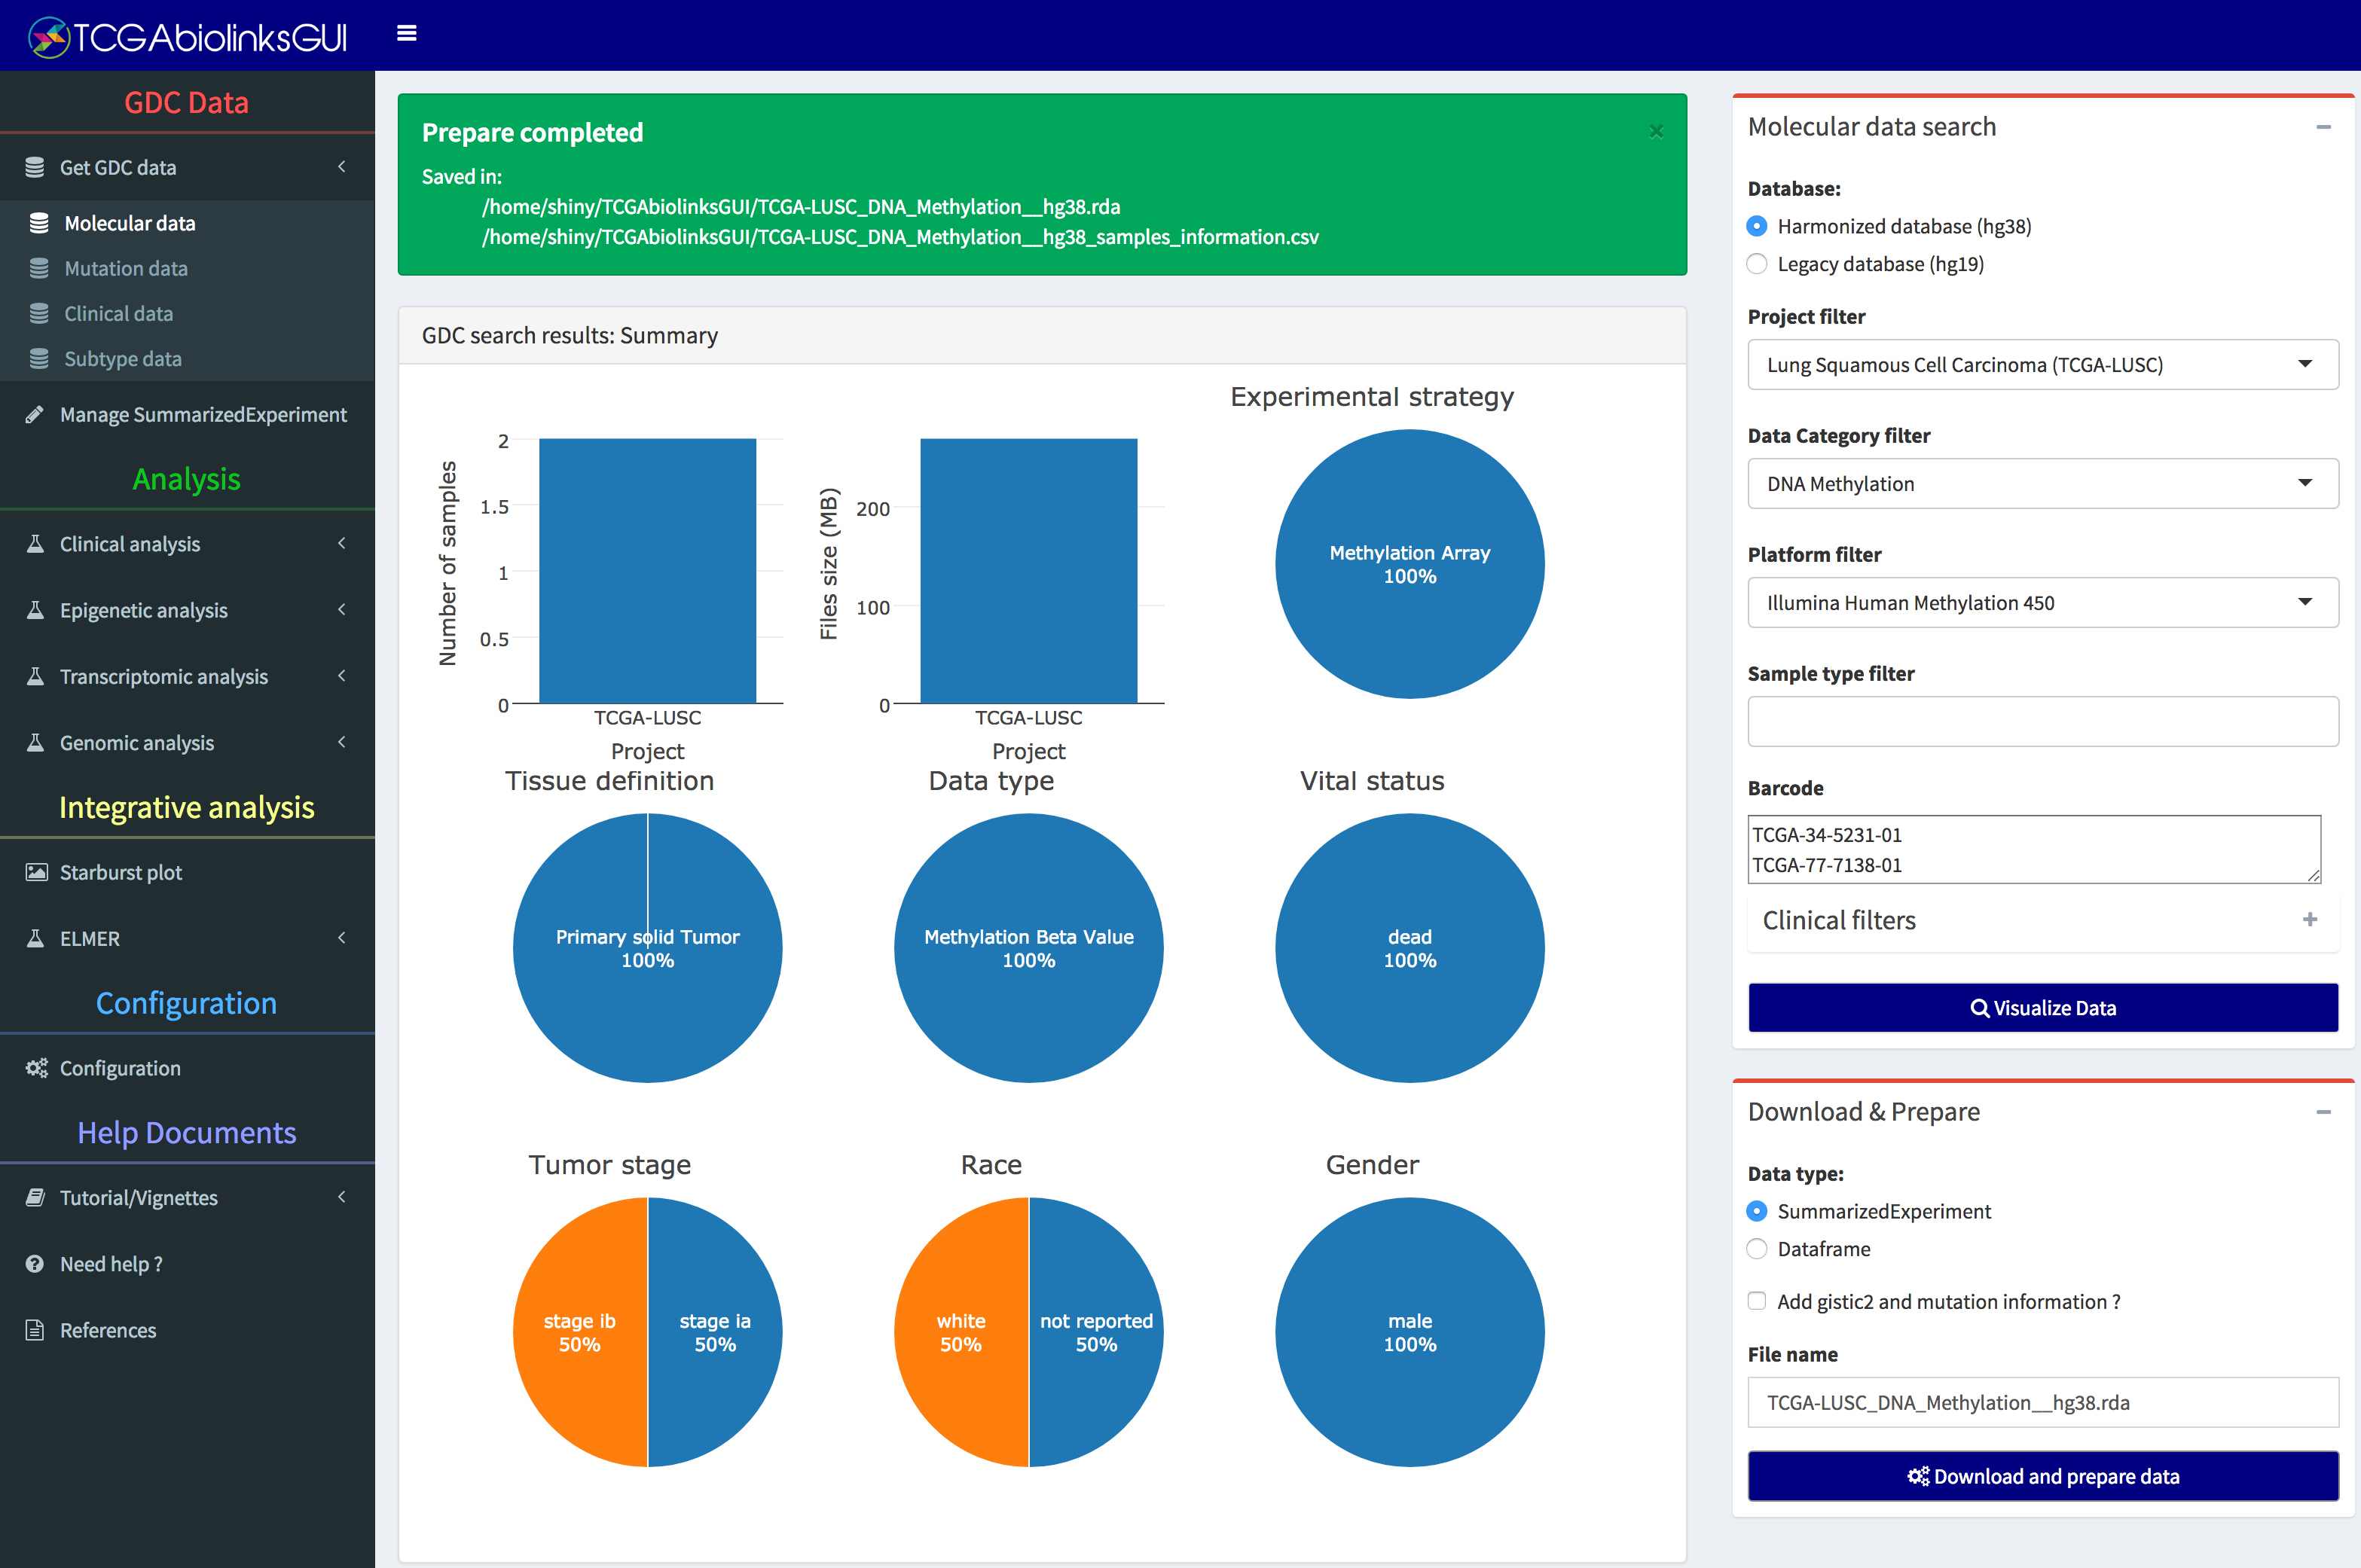
\includegraphics[width=1.0\linewidth]{TCGAbiolinks/GUI.png}
 \end{figure}
\end{frame}




\section{ELMER}
\begin{frame}{Enhancer-mediated gene regulation}
 \vspace*{1.0cm}
 \begin{figure}
  \centering
  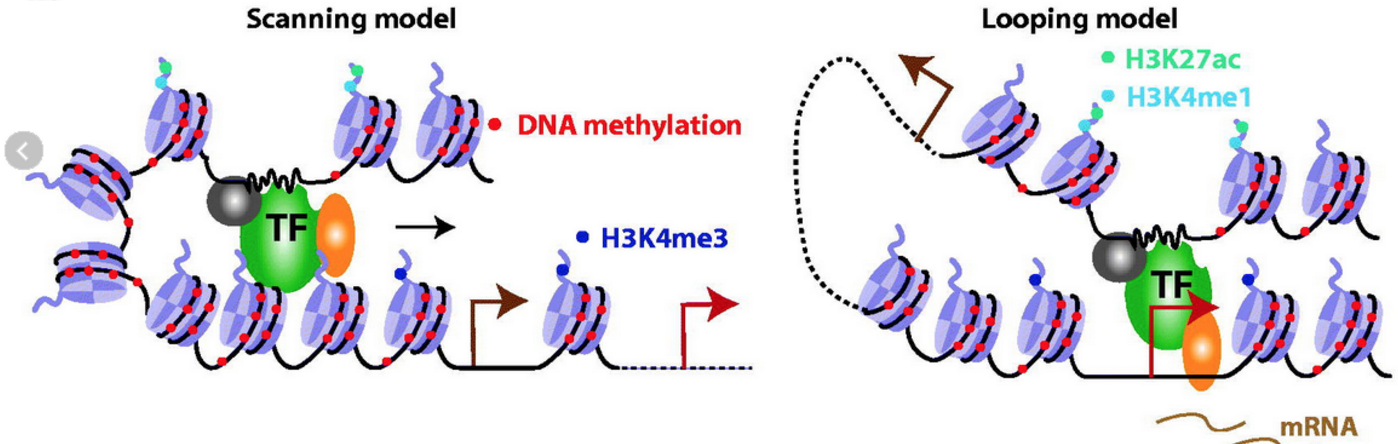
\includegraphics[width=1.0\linewidth]{ELMER/elmer.png}{\tiny{\\\href{https://genomebiology.biomedcentral.com/articles/10.1186/s13059-015-0668-3}{Yao et al. Genome Biology (2015) 16:105.}}}
 \end{figure}
 \pdfnote{\tiny{ scanning or tracking model: TF  binds at an enhancer and moves along the genome, searching for a target promoter }}
 \pdfnote{\tiny{  looping model:  enhancer directly interacts with a target promoter by forming a DNA loop }}

\end{frame}



\begin{frame}{Enhancer-mediated gene regulation}
 \begin{itemize}
  \item 73\% of the tested distal elements do not link to the nearest gene (Sanyal et al., 2012)
  \item 40\% of the enhancers involved in loops do not interact with the TSS of the nearest gene (Li et al., 2012),
  \item one-third of the distal interactions were not directed to the promoter of the nearest gene (Mifsud et al., 2015),
  \item 85\% of tumor-specific enhancers that could be linked to the expression of a nearby gene skipped the nearest gene (Yao et al., 2015).
 \end{itemize}
\end{frame}

\begin{frame}{Enhancer-mediated gene regulation}
 \vspace*{-0.1cm}
 \begin{figure}
  \centering
  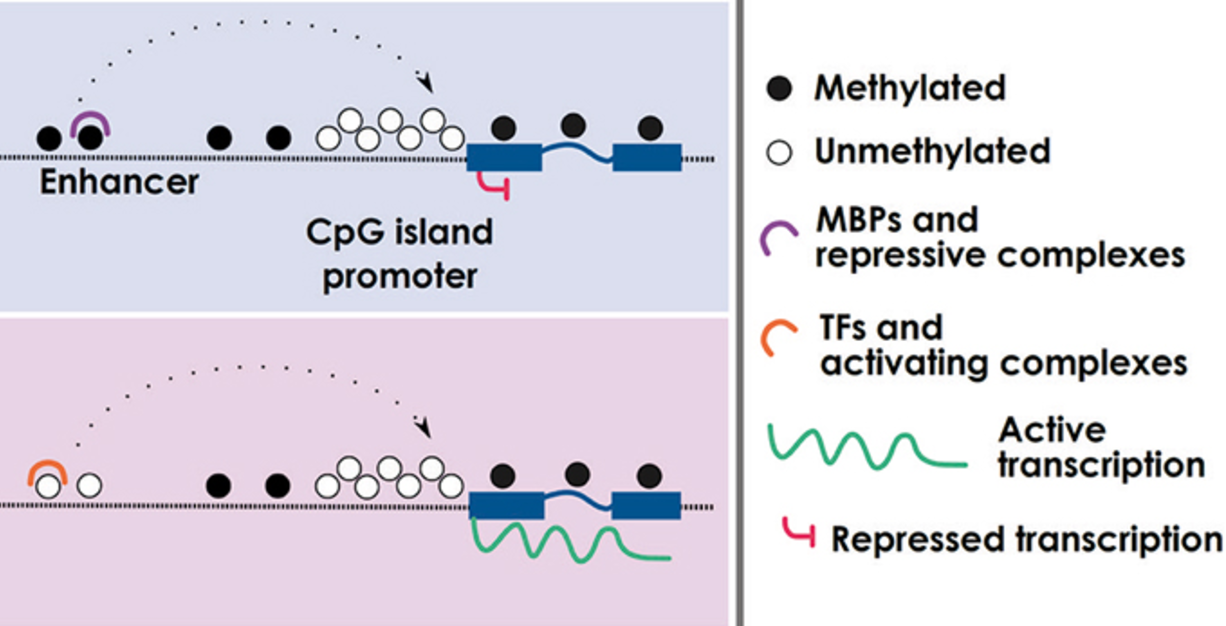
\includegraphics[width=1.0\linewidth]{ELMER/dna_met.png}{\tiny{\\Source: Front. Aging Neurosci., 05 March 2015 http://dx.doi.org/10.3389/fnagi.2015.00019.}}
 \end{figure}
\end{frame}

\begin{frame}{ Enhancer Linking by Methylation/Expression Relationship}
 \vspace*{-0.5cm}
 \begin{figure}
  \centering
  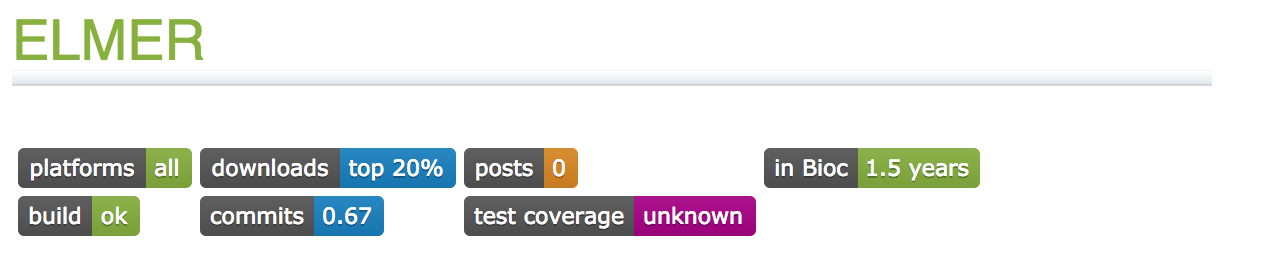
\includegraphics[width=0.8\linewidth]{ELMER/elmer1.png}
 \end{figure}
 \vspace*{-0.5cm}
 \begin{figure}
  \centering
  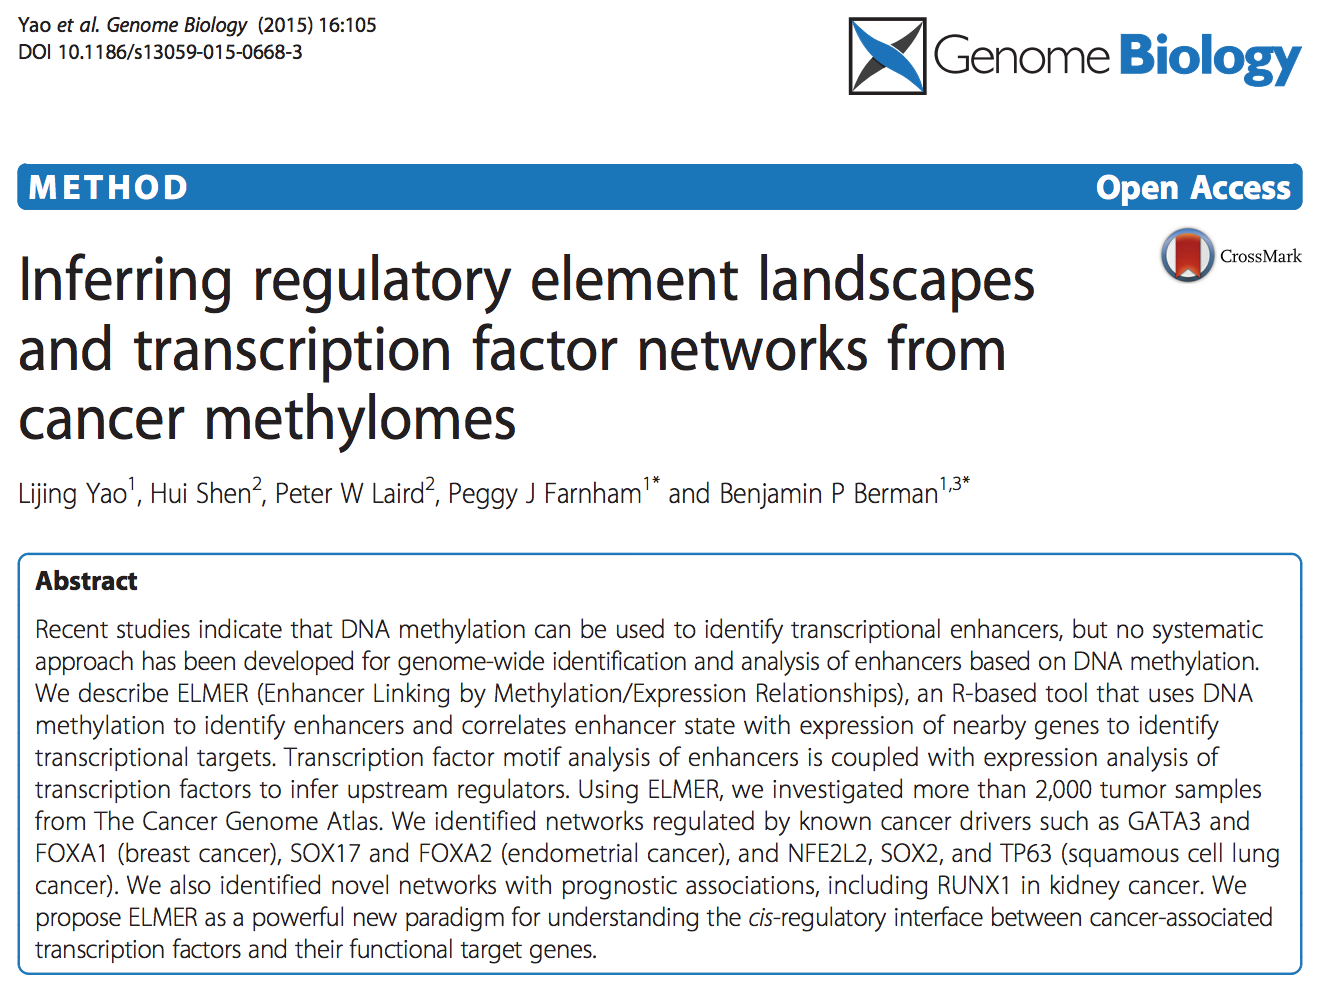
\includegraphics[width=0.8\linewidth]{ELMER/elmer2.png}
 \end{figure}
\end{frame}



\begin{frame}[plain]%{Workflow}
 \vspace*{-0.3cm}
 \begin{figure}
  \centering
  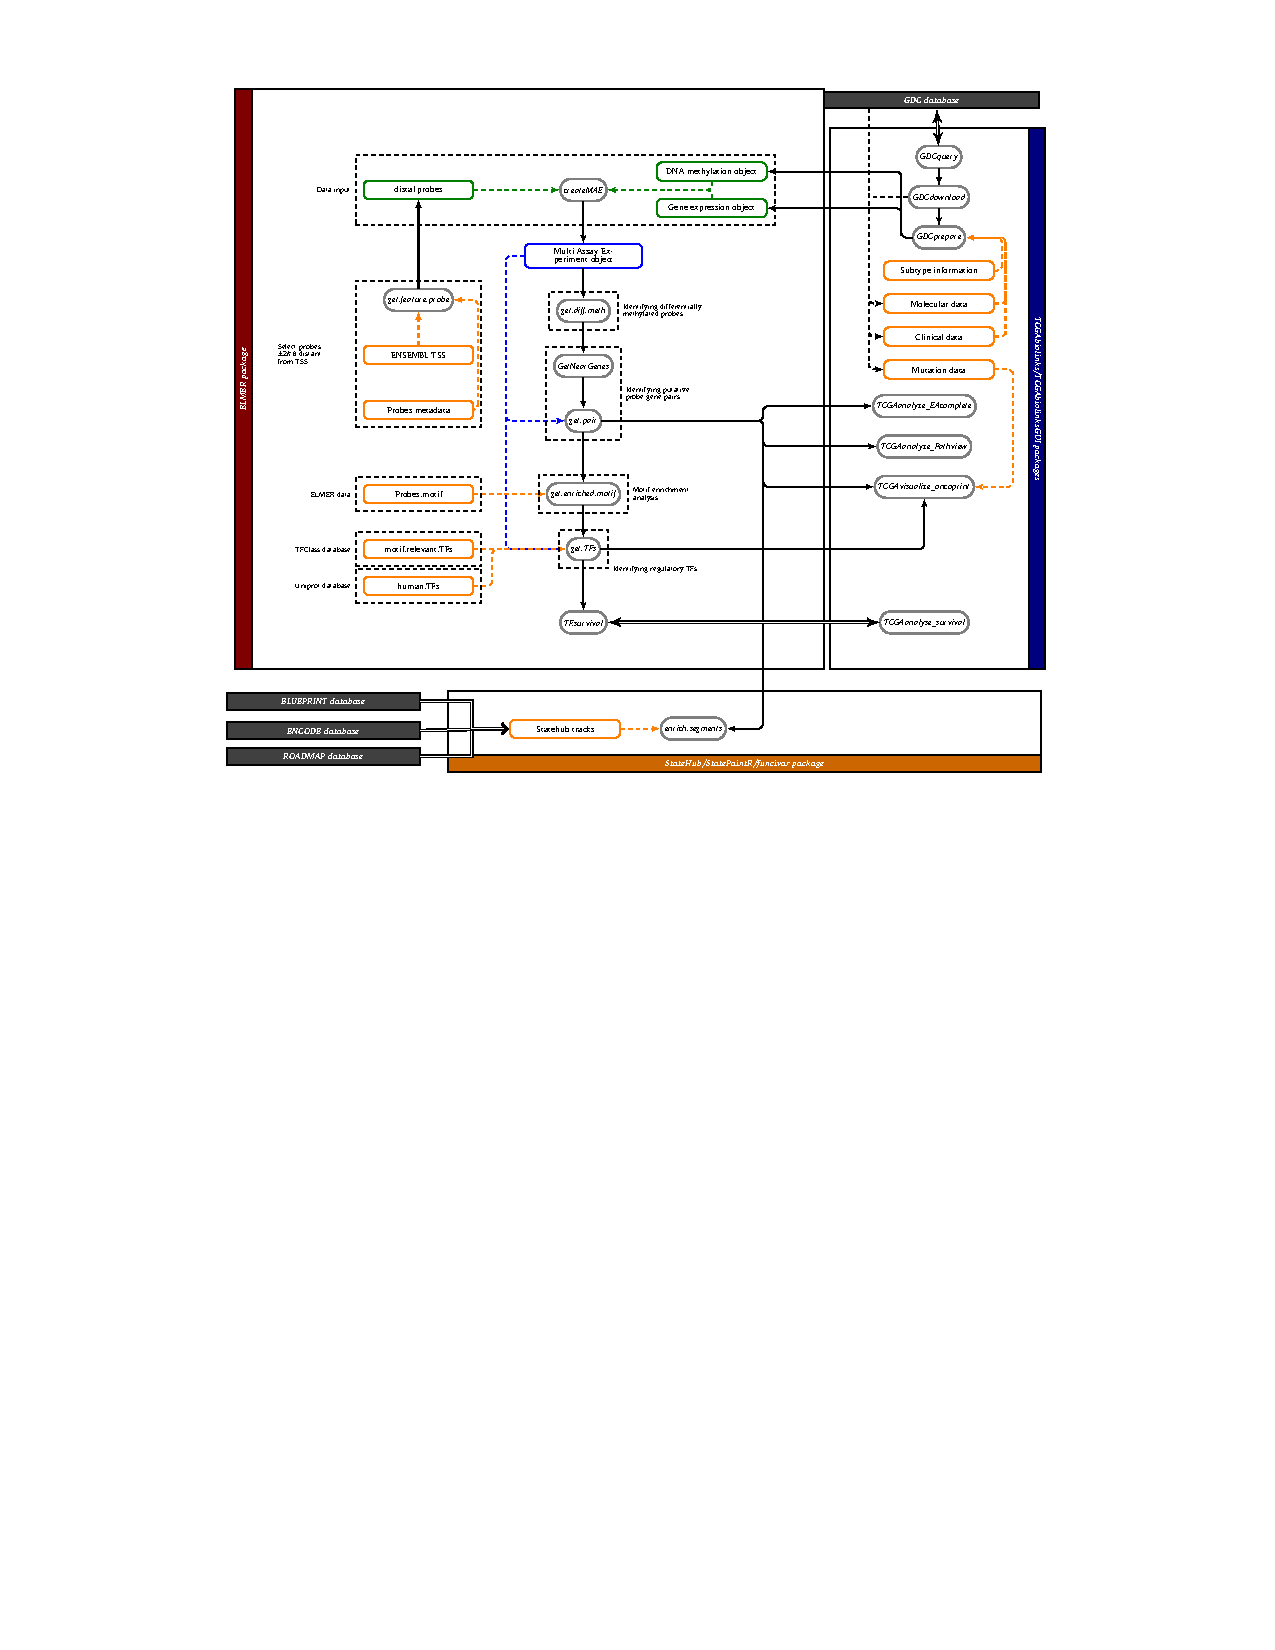
\includegraphics[width=1.0\linewidth]{ELMER/workflow.pdf}
 \end{figure}
\end{frame}


%\begin{frame}{Algorithm}

%\begin{exampleblock}{Steps}
%\begin{enumerate}
%\item  Identify distal  probes on HM450K/EPIC.
%\item  Identify distal  probes with significantly different DNA methylation level in  group 1 compared to group 2.
%\item  Identify putative target genes for differentially methylated distal enhancer probes.
%\item  Identify enriched motifs for the distal  probes which are significantly differentially methylated and linked to putative target gene.
%\item  Identify regulatory TFs whose expression associate with DNA methylation at motifs.
%\end{enumerate}

%\end{exampleblock}


%\end{frame}


\begin{frame}{Step 1: Identify distal probes}
 %\vspace*{1.0cm}
 \begin{figure}
  \centering
  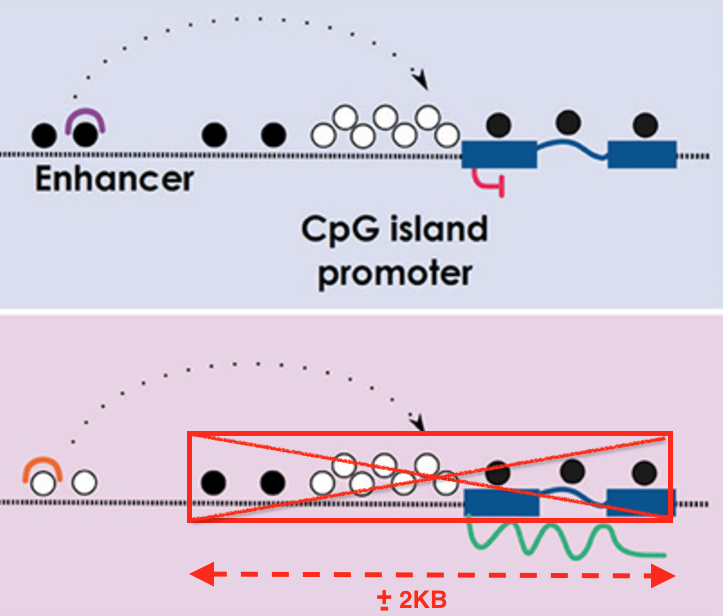
\includegraphics[width=0.7\linewidth]{step1.png}
 \end{figure}
\end{frame}


\begin{frame}{Step 2: Differentially methylated distal probes}
 \vspace*{-0.3cm}
 \begin{figure}
  \centering
  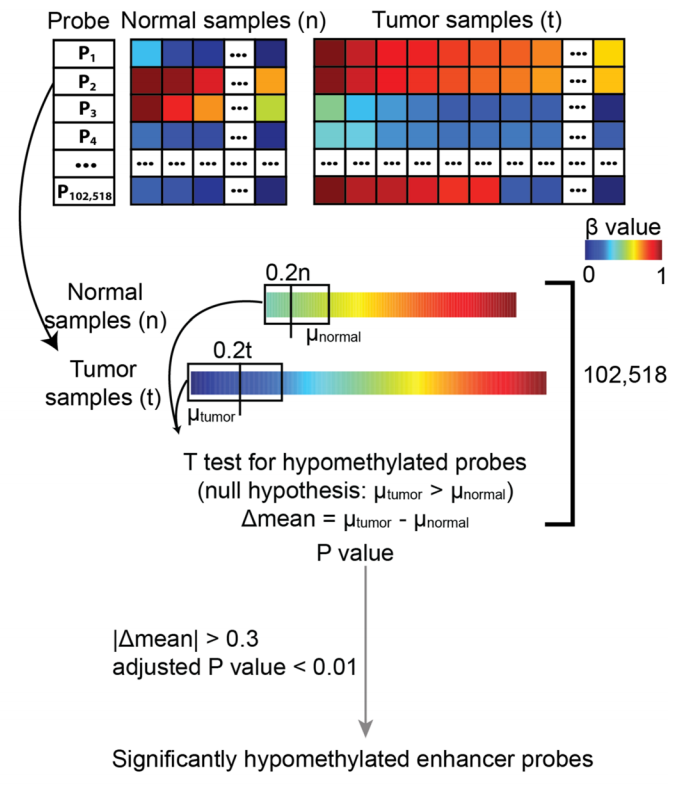
\includegraphics[width=0.5\linewidth]{ELMER/diffmeth.png}{\tiny{\\Yao et al. Genome Biology (2015) 16:105.}}
 \end{figure}
\end{frame}


\begin{frame}{Step 2: Differentially methylated distal probes}
 \begin{figure}
  \centering
  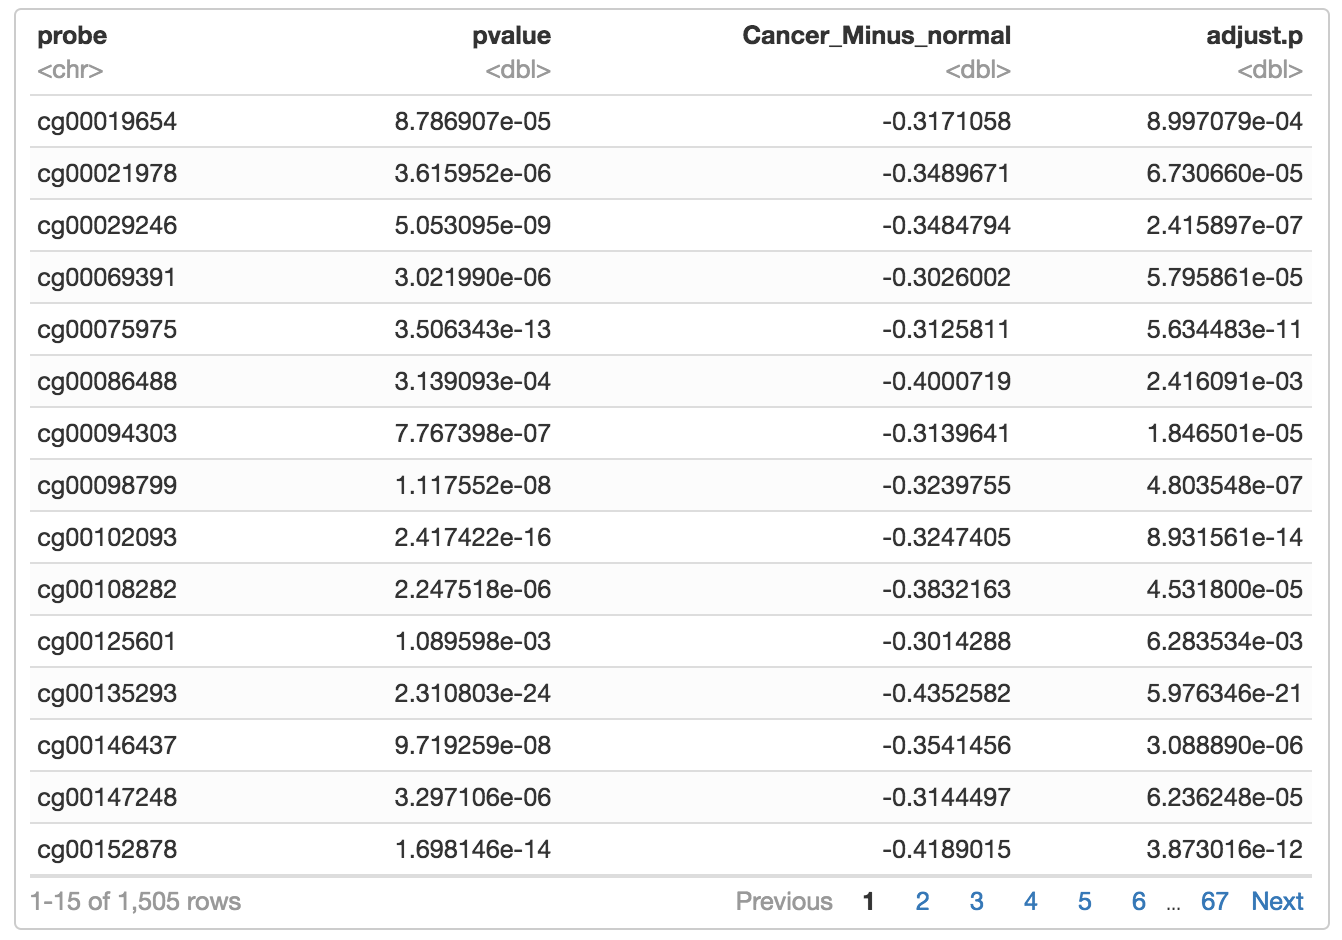
\includegraphics[width=0.9\linewidth]{ELMER/metdiff_tbl.png}
 \end{figure}
\end{frame}

\begin{frame}{Step 2: Differentially methylated distal probes}
 \begin{figure}
  \centering
  \includegraphics[width=1.0\linewidth]{ELMER/volcano_plot.pdf}
 \end{figure}
\end{frame}

\begin{frame}{Step 3: Identification of putative target gene(s)}
 \vspace*{-0.3cm}
 \begin{figure}
  \centering
  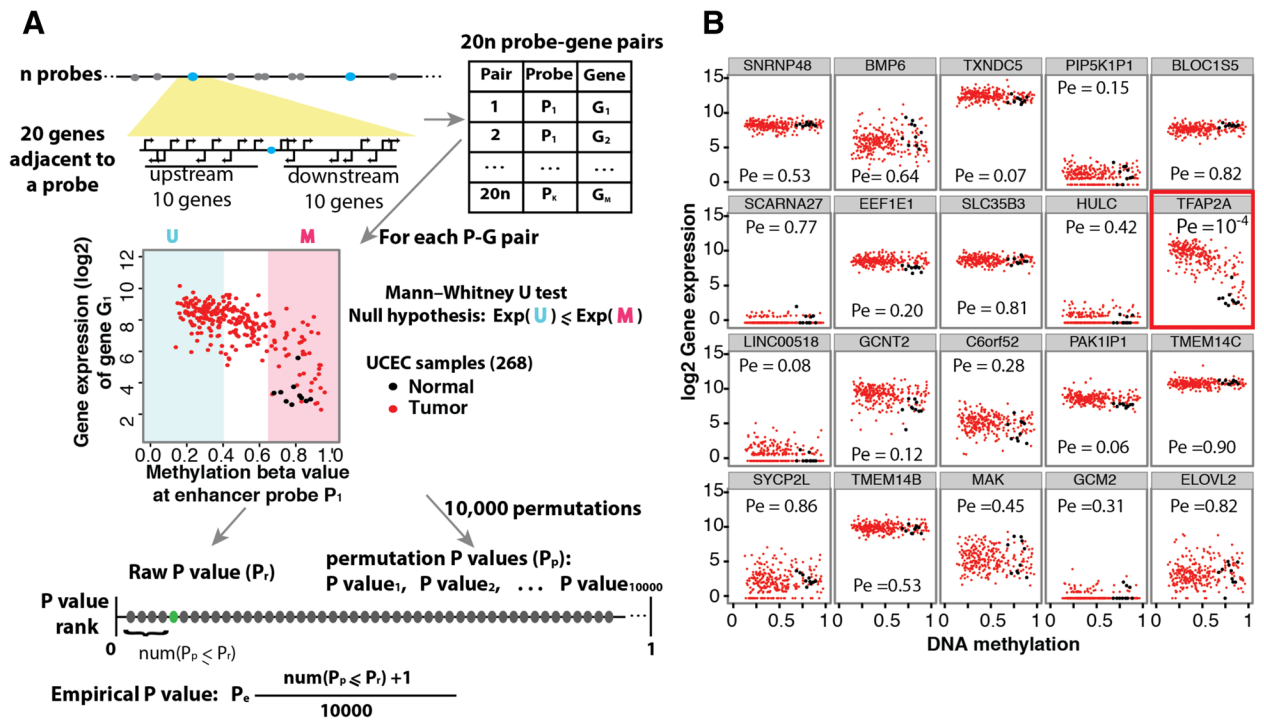
\includegraphics[width=1.0\linewidth]{ELMER/pair.png}{\tiny{\\Yao et al. Genome Biology (2015) 16:105.}}
 \end{figure}
\end{frame}



\begin{frame}{Step 3: Probe-target gene pairs inferred}
 \begin{figure}
  \centering
  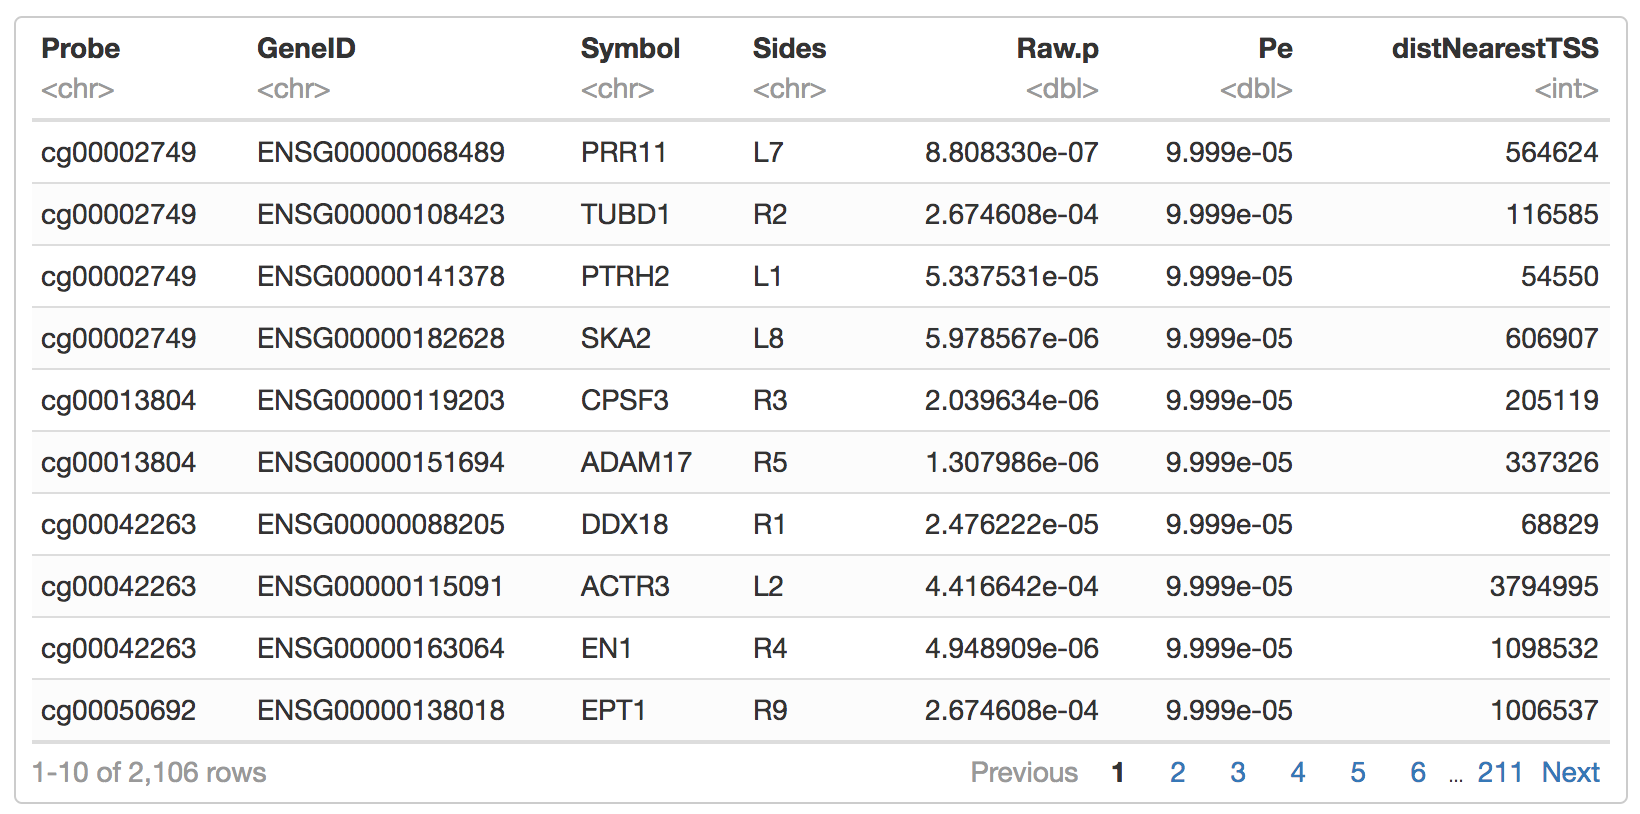
\includegraphics[width=1.0\linewidth]{ELMER/pairs_tbl.png}
 \end{figure}
\end{frame}

\begin{frame}{Step 3: Probe-target gene pairs inferred}
 \vspace*{-0.3cm}
 \begin{figure}
  \centering
  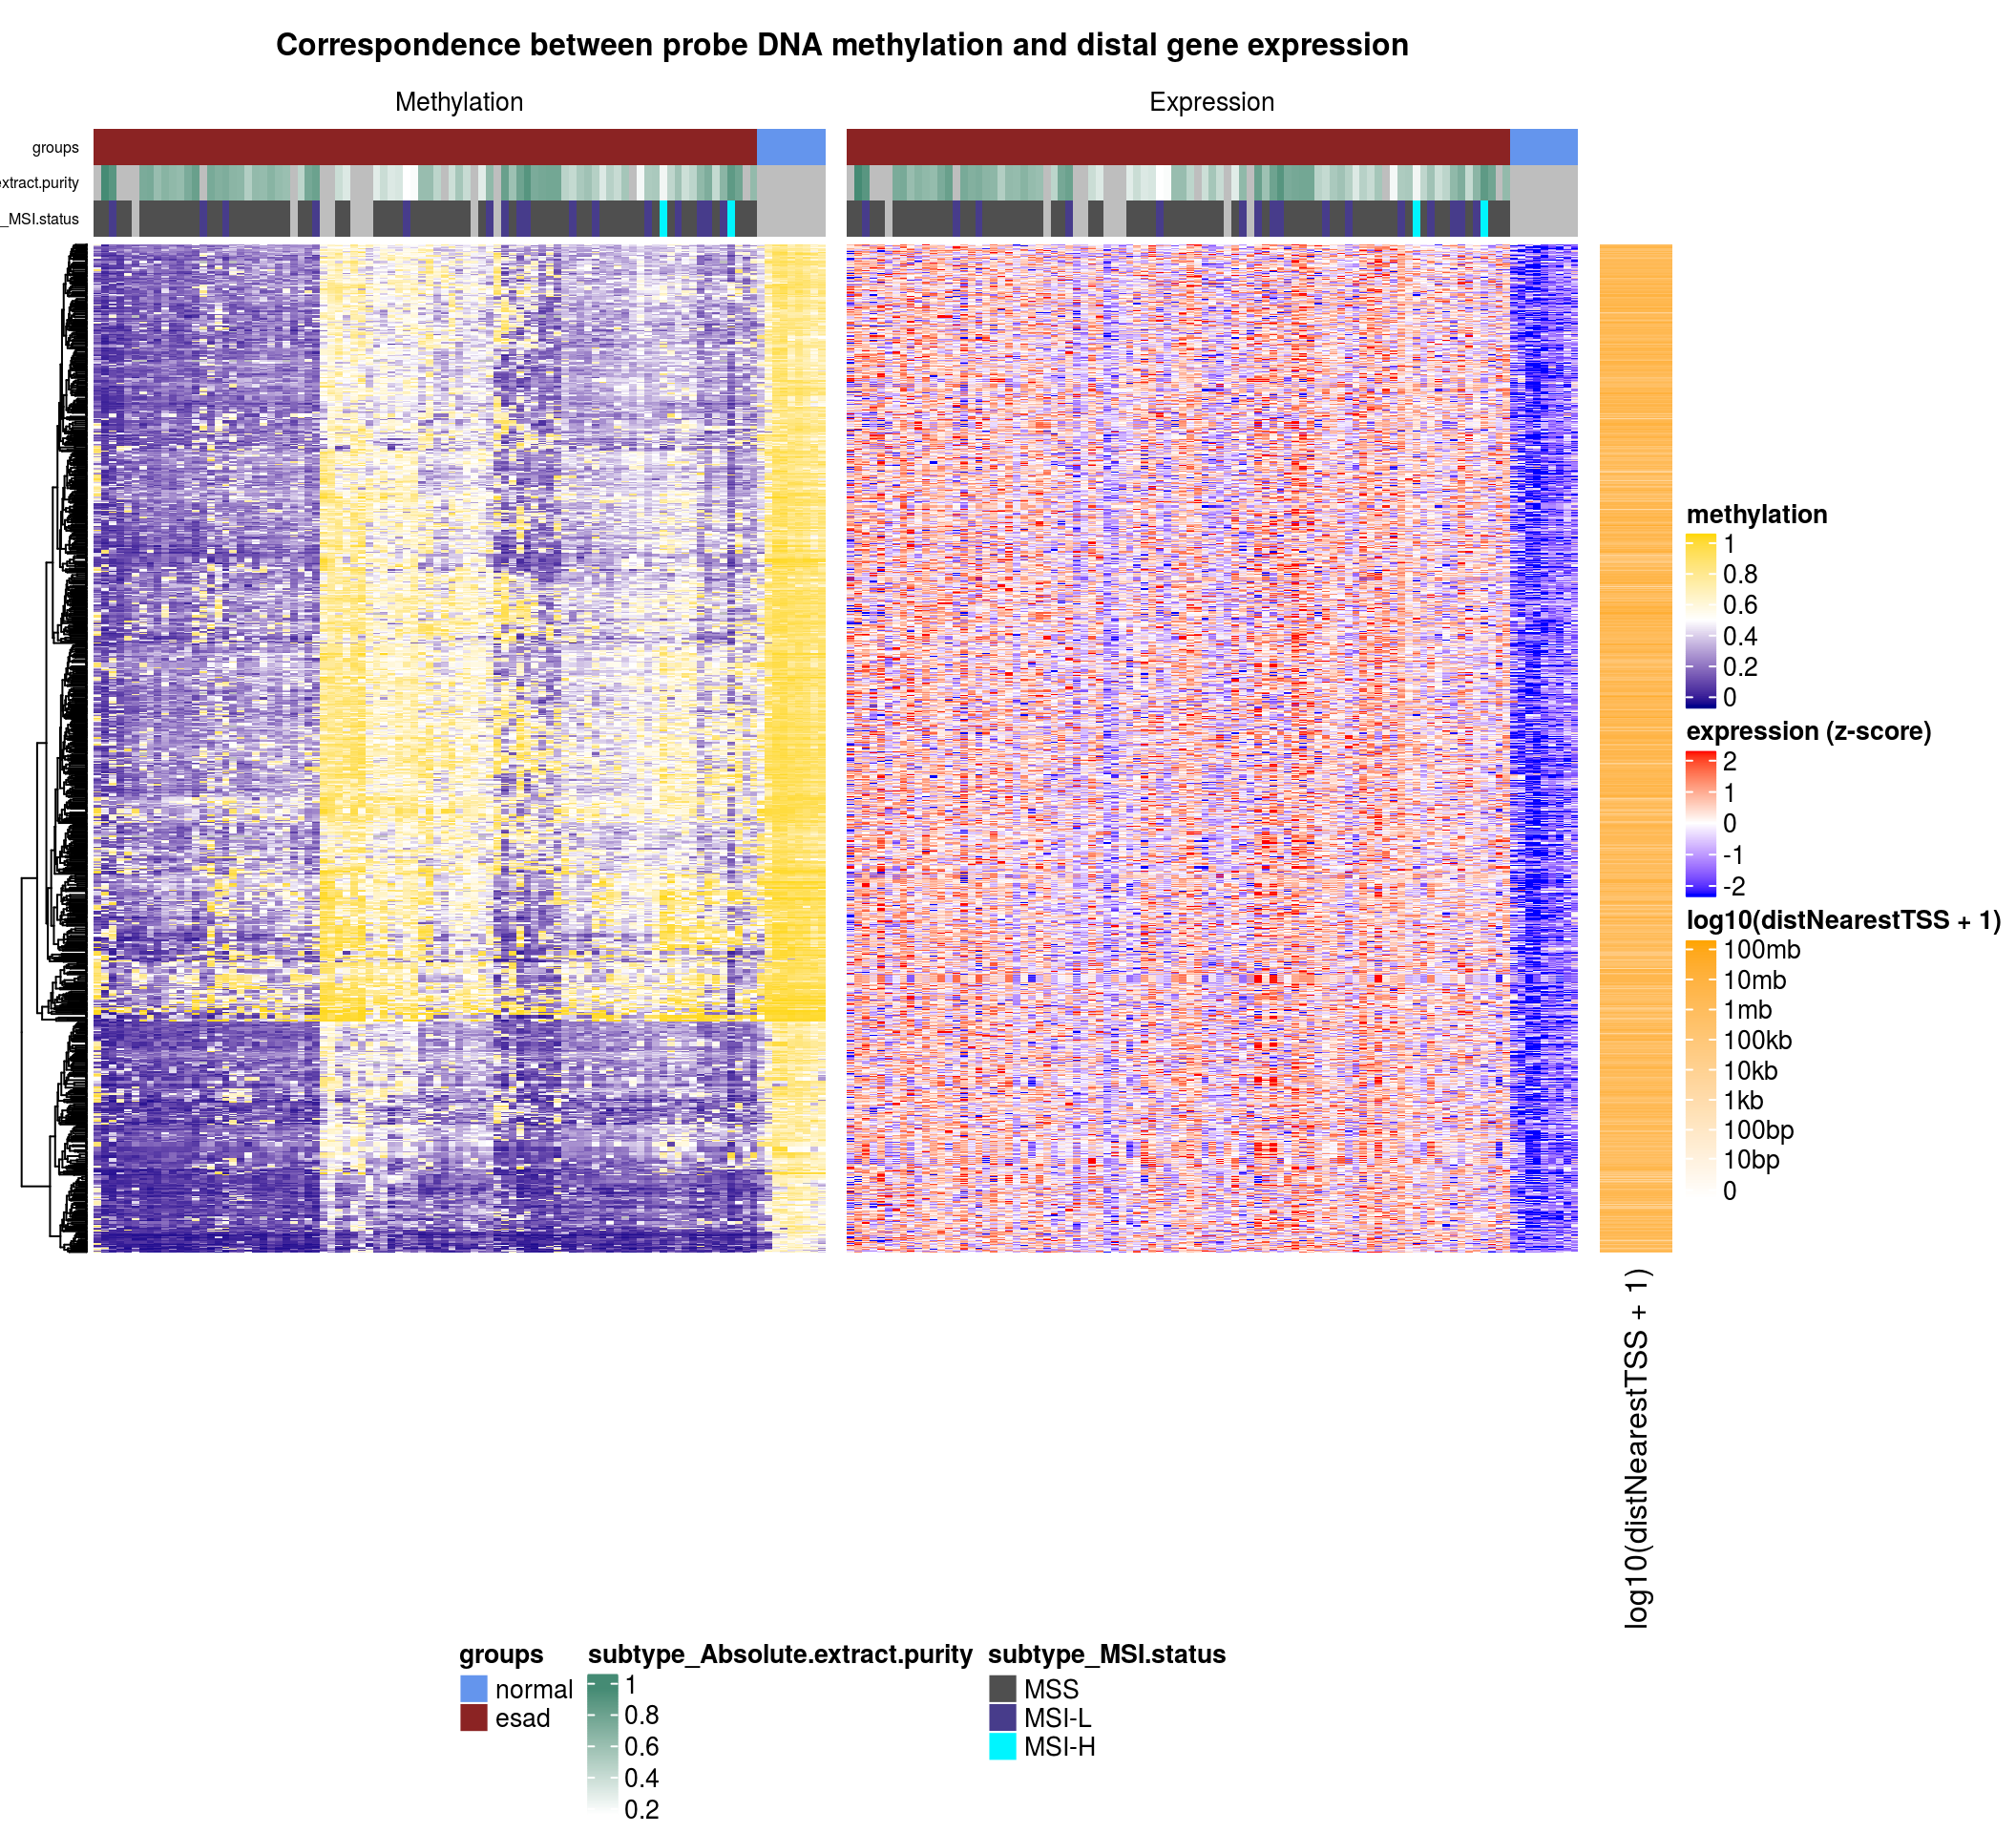
\includegraphics[width=0.75\linewidth]{ELMER/heatmappair.png}
 \end{figure}
\end{frame}


\begin{frame}{Step 4: Motif enrichment analysis}

 \vspace*{-0.3cm}
 \begin{figure}
  \centering
  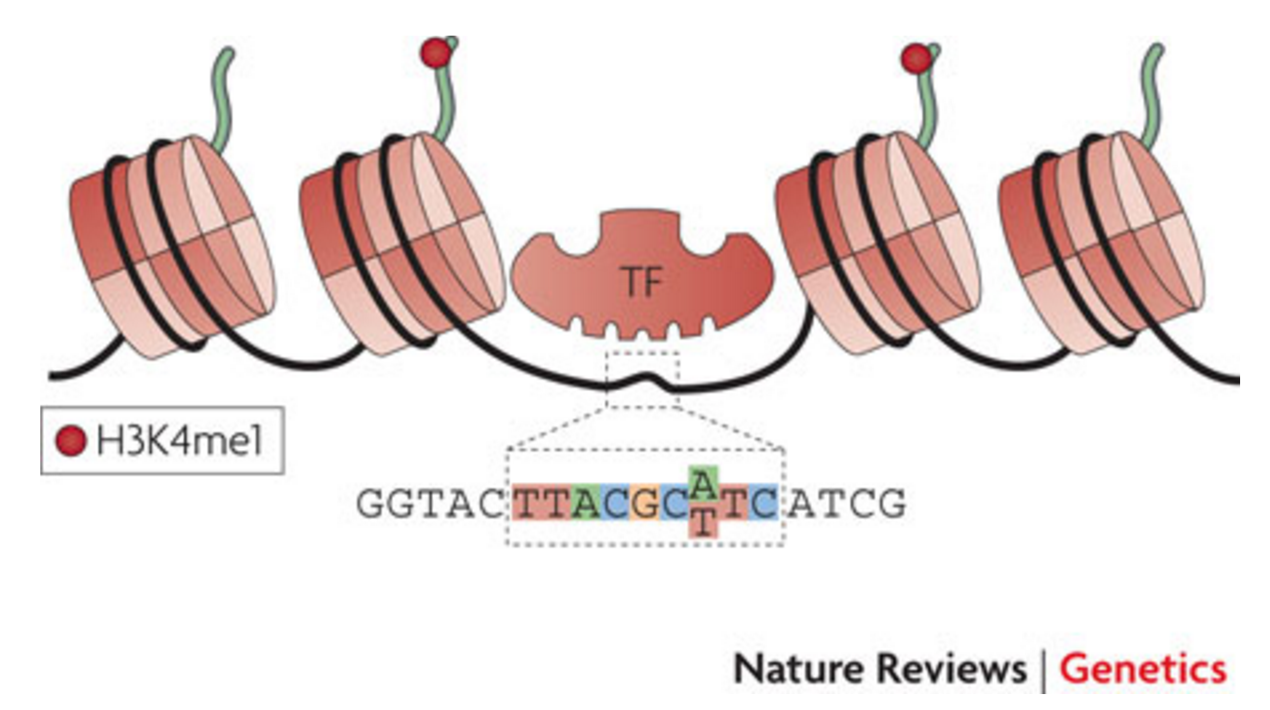
\includegraphics[width=1.0\linewidth]{ELMER/tf_binding.png}{\tiny{\\Next-generation genomics: an integrative approach R. David Hawkins et al. Nature Reviews Genetics 11, 476-486}}
 \end{figure}
\end{frame}


\begin{frame}{Step 4:  TF motifs source}
 \vspace*{-0.3cm}
 \begin{figure}
  \centering
  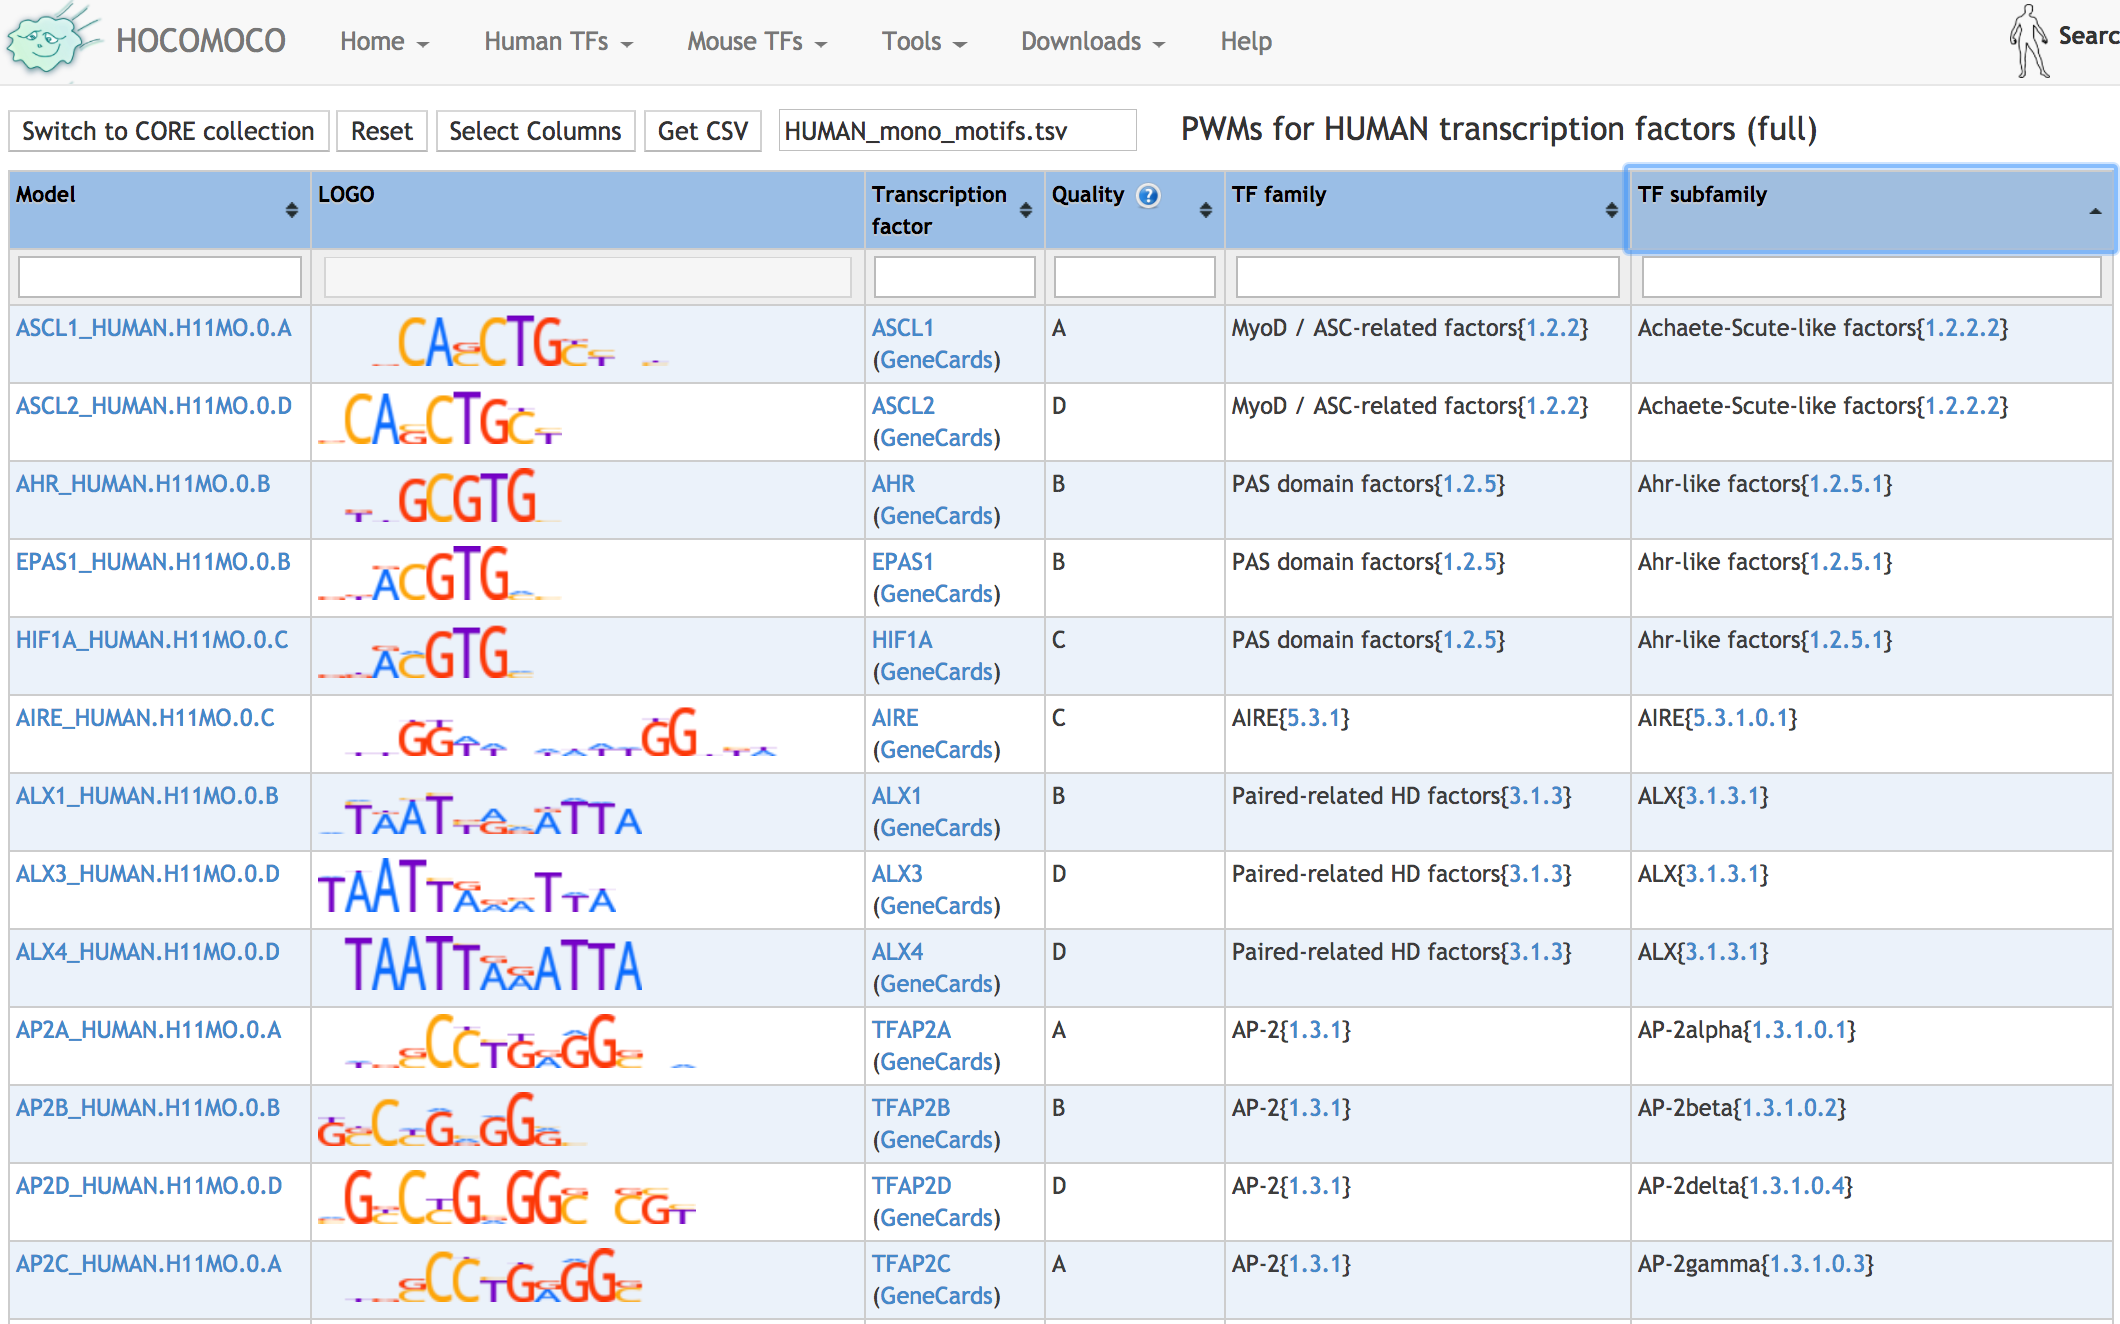
\includegraphics[width=1.0\linewidth]{ELMER/hocomoco.png}{\tiny{\\HOCOMOCO v11 (http://hocomoco11.autosome.ru/human/mono?full=true), Accessed: 25-12-2017}}
 \end{figure}
\end{frame}

\begin{frame}{Step 4: Motif enrichment analysis}

\begin{block}{Objective}
Evaluate the enrichment of transcription factors in certain genomic regions.
\begin{enumerate}
  \item Perform motif matching of transcription factors in probes regions (window $\pm250bp$). Performed using HOMER (Hypergeometric Optimization of Motif EnRichment) with HOCOMOCO motifs.
  \item Evaluate which transcription factors are more likely to occur in those regions than in background regions
  using Fisher’s exact test with FDR correction.
\end{enumerate}
\end{block}
 \begin{exampleblock}{Fisher’s exact test}
 a: nb of input regions with match for TF motif.\\
 b: nb of input regions with no match for TF motif.\\
 c: nb of background regions with match for TF motif.\\
 d: nb of background regions with no match for TF motif.
 \end{exampleblock}

\end{frame}

\begin{frame}{Step 4: Motif enrichment analysis}
 \begin{figure}
  \centering
  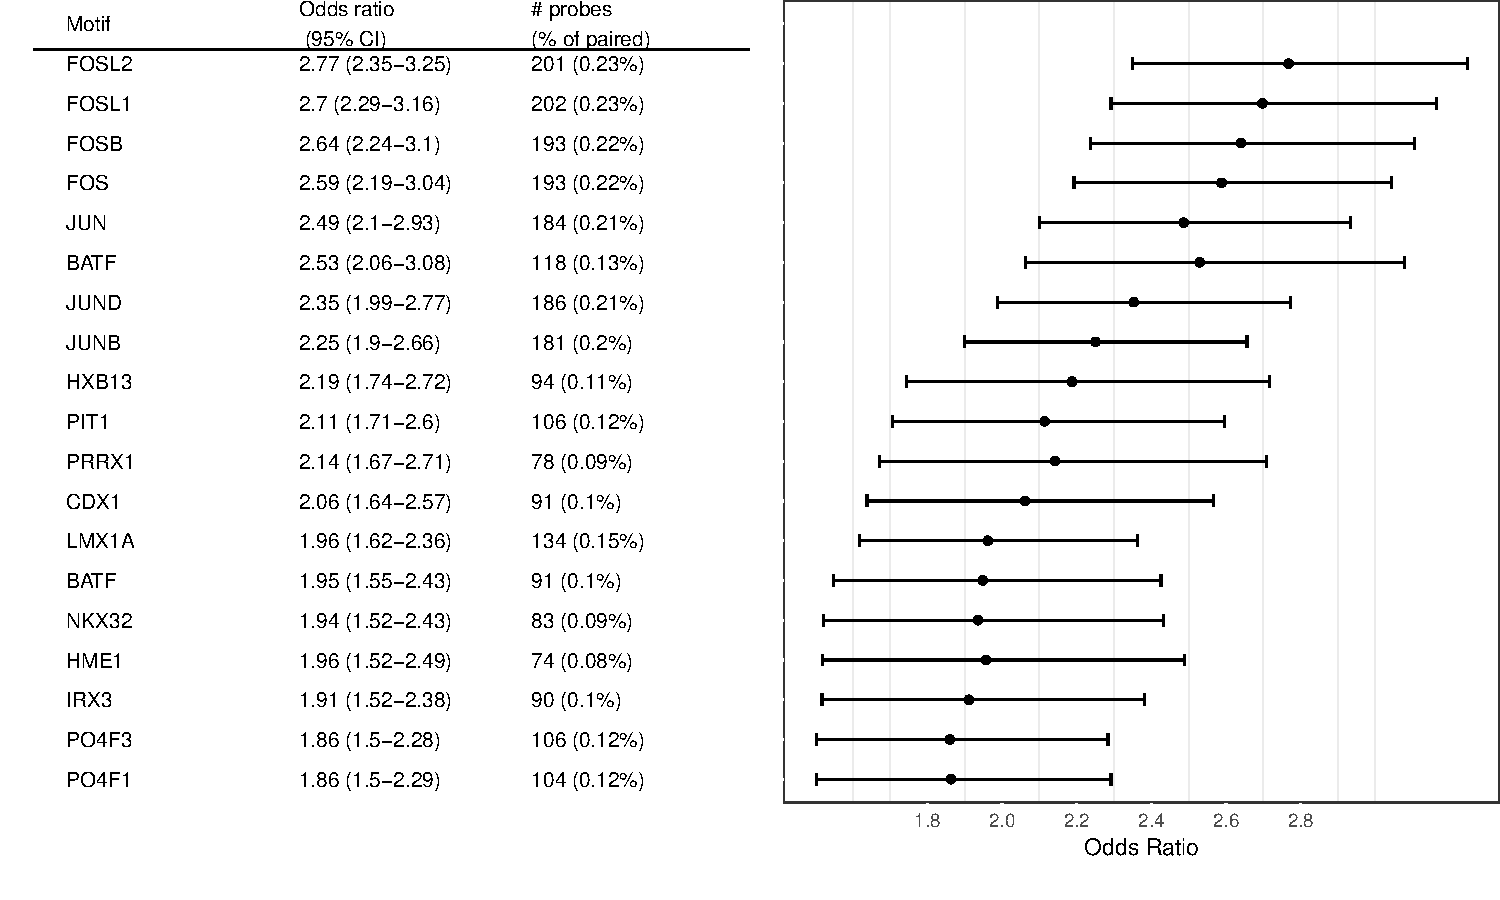
\includegraphics[width=1.0\linewidth]{ELMER/motif_enrichment.pdf}
 \end{figure}
\end{frame}

\begin{frame}{Step 4: Motif enrichment analysis}
 \begin{figure}
  \centering
  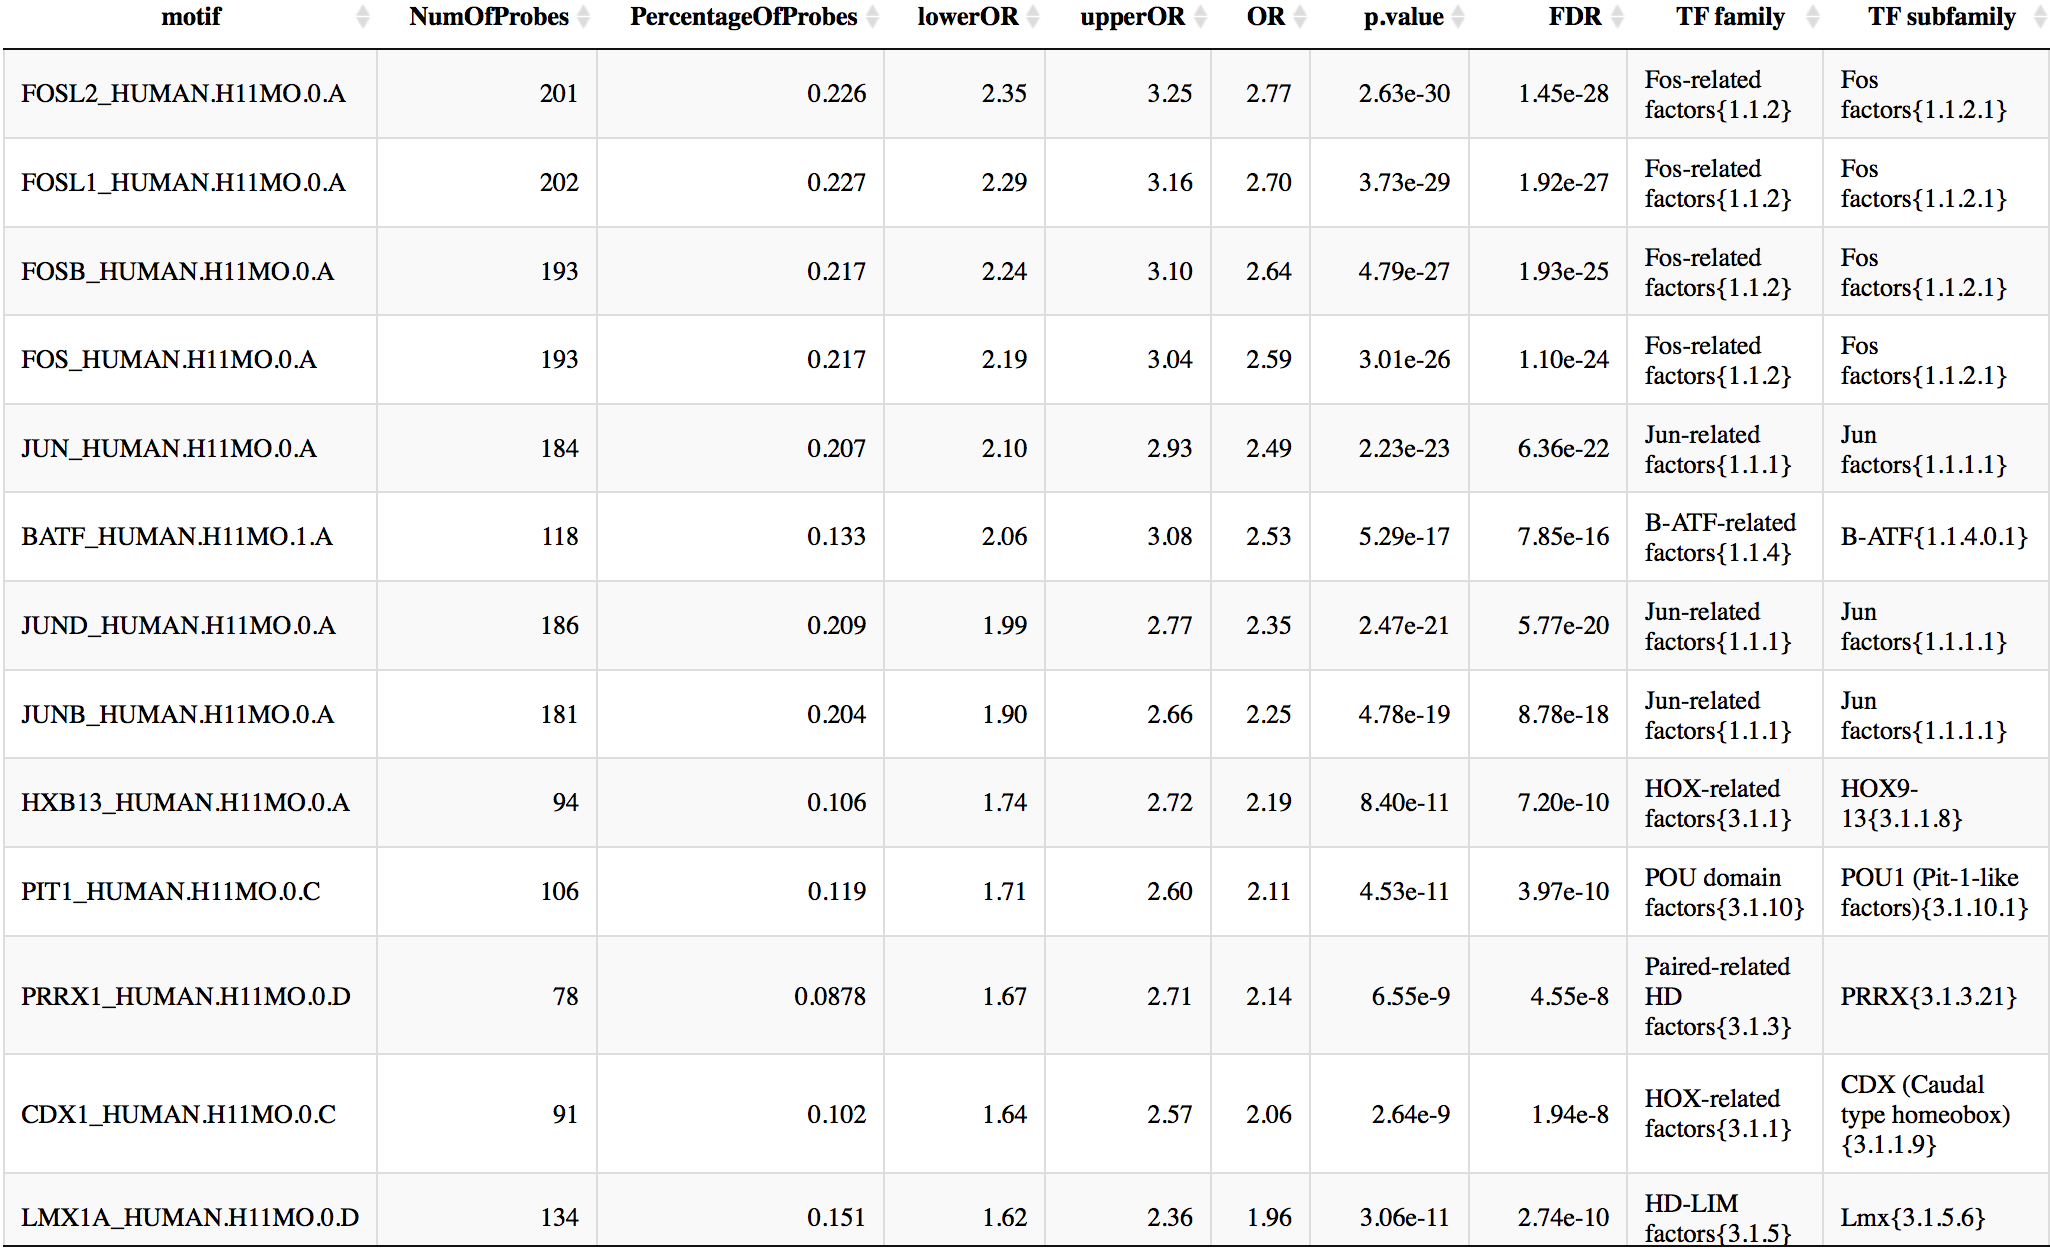
\includegraphics[width=1.0\linewidth]{ELMER/or_tbl.png}
 \end{figure}
\end{frame}


\begin{frame}{Step 5: Human TFs}
 \vspace*{-0.3cm}
 \begin{figure}
  \centering
  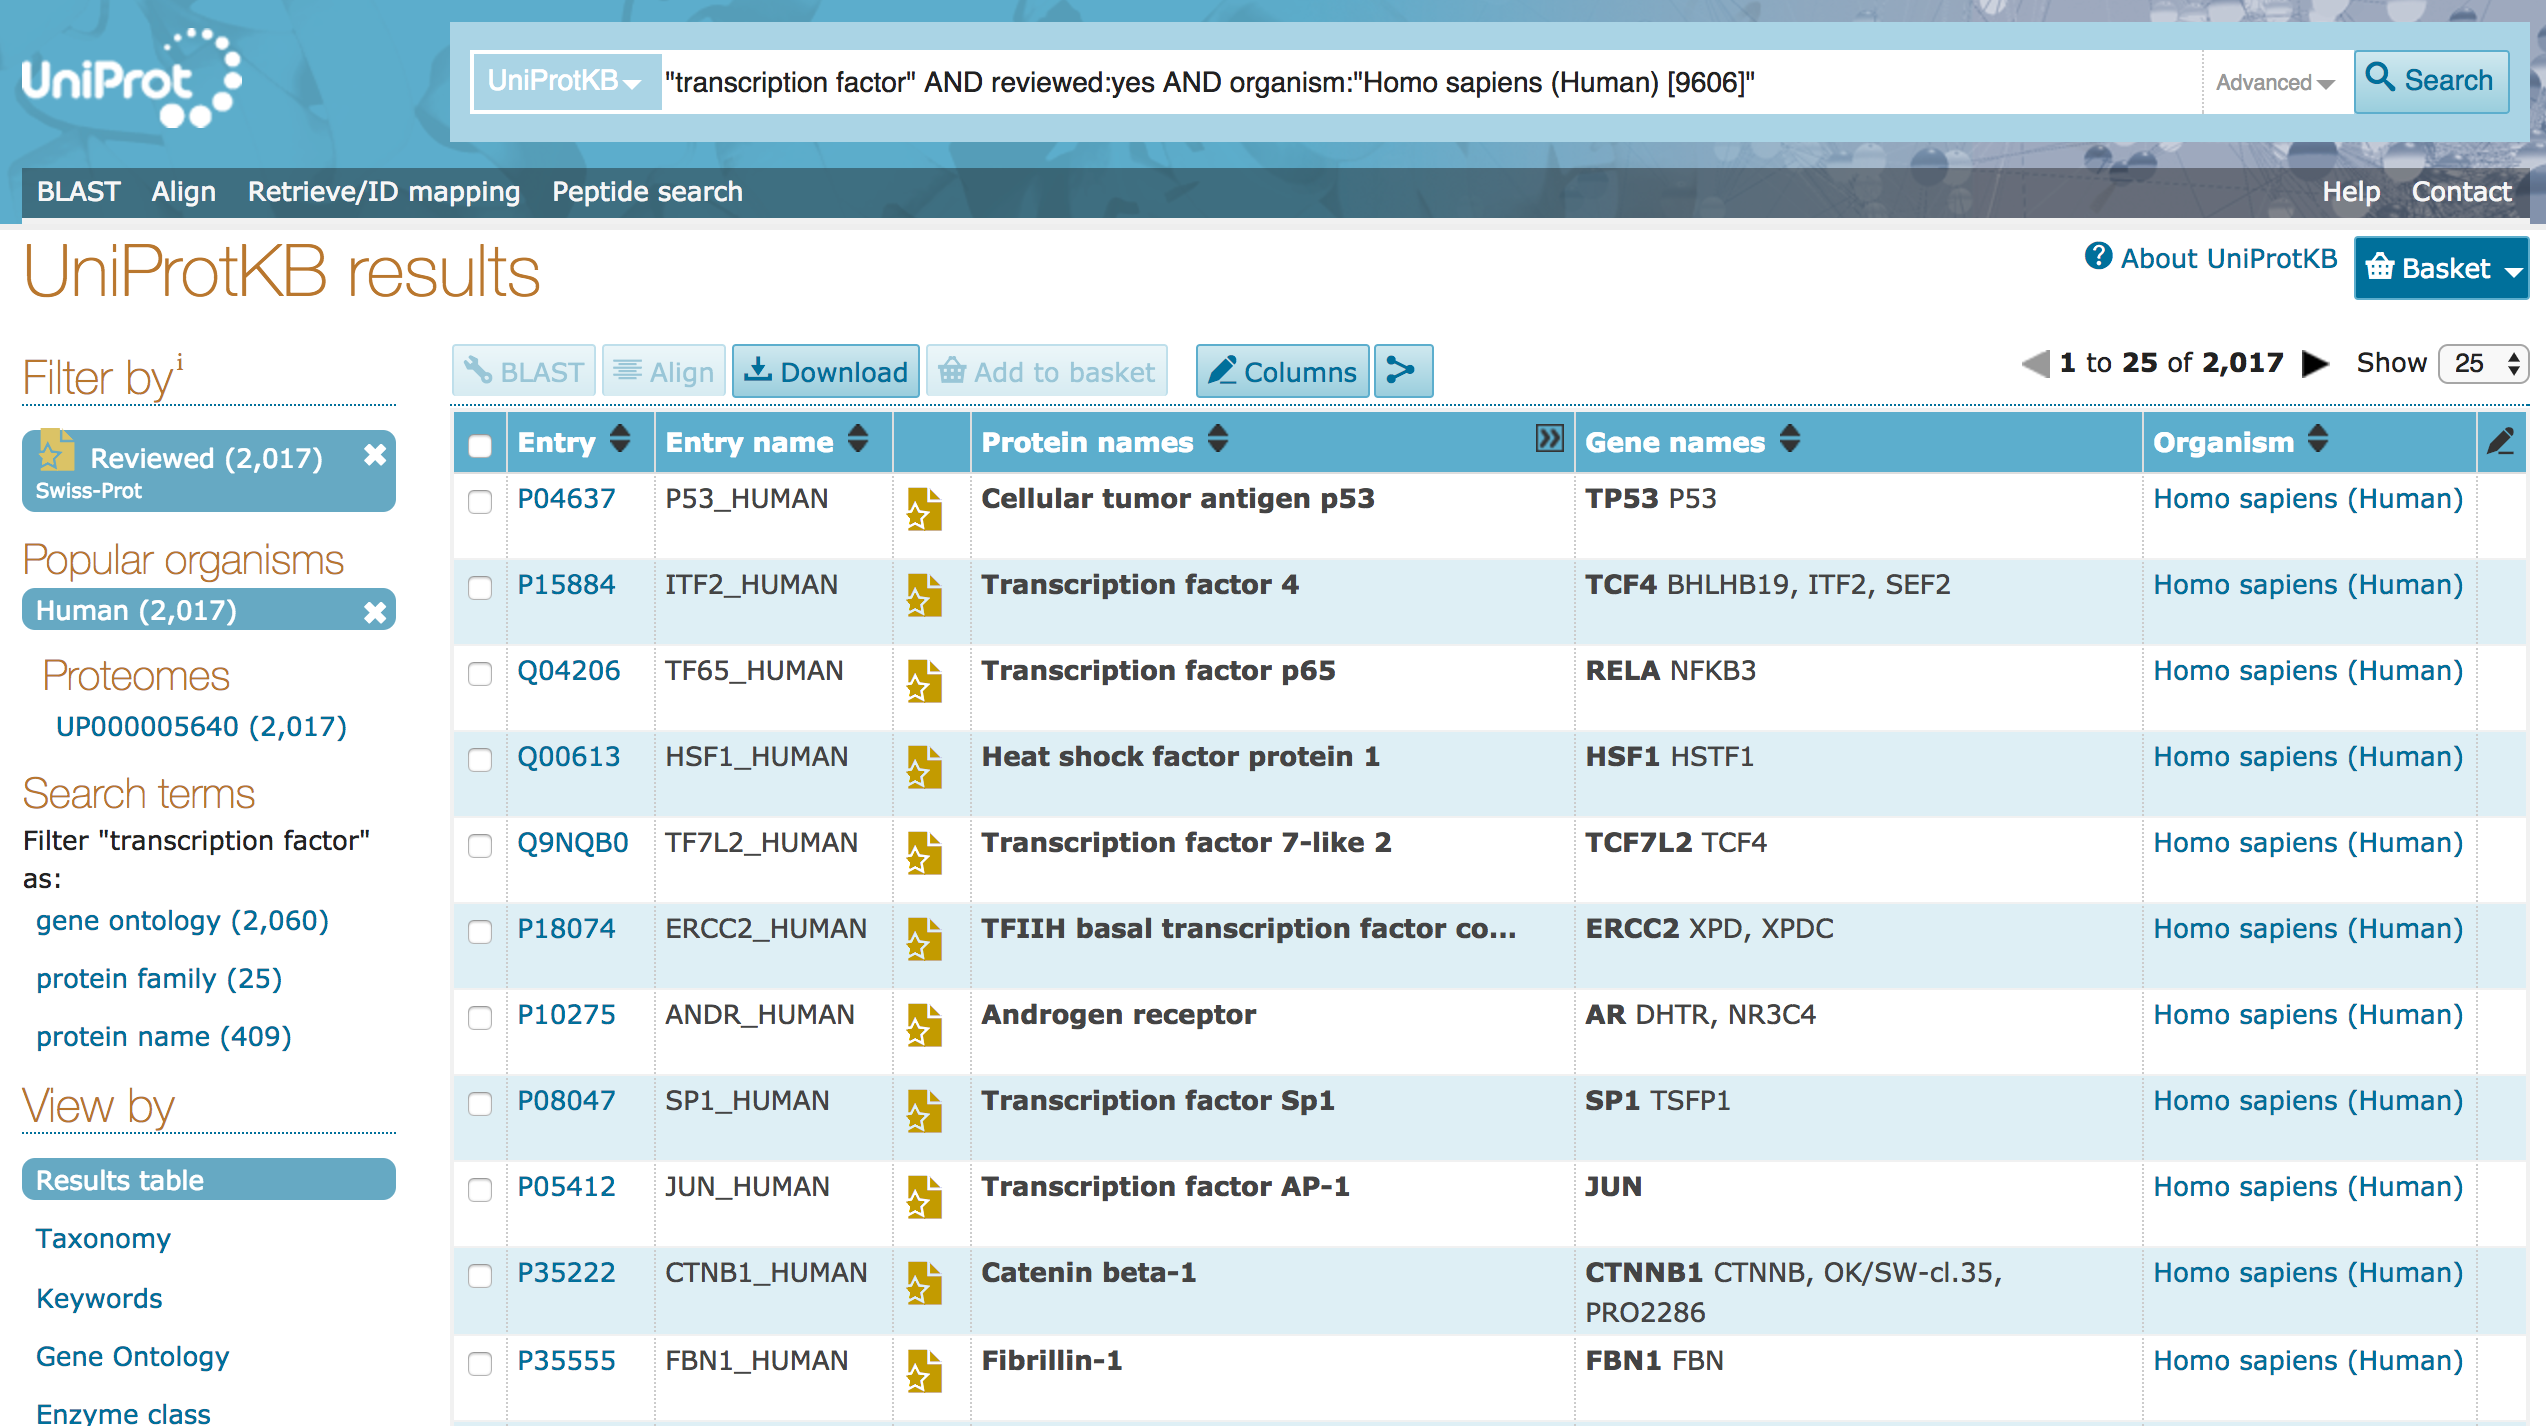
\includegraphics[width=1.0\linewidth]{ELMER/uniprot.png}
 \end{figure}
\end{frame}

\begin{frame}{Step 5: Identification of master regulator TF}
 \vspace*{-0.5cm}
 \begin{figure}
  \centering
  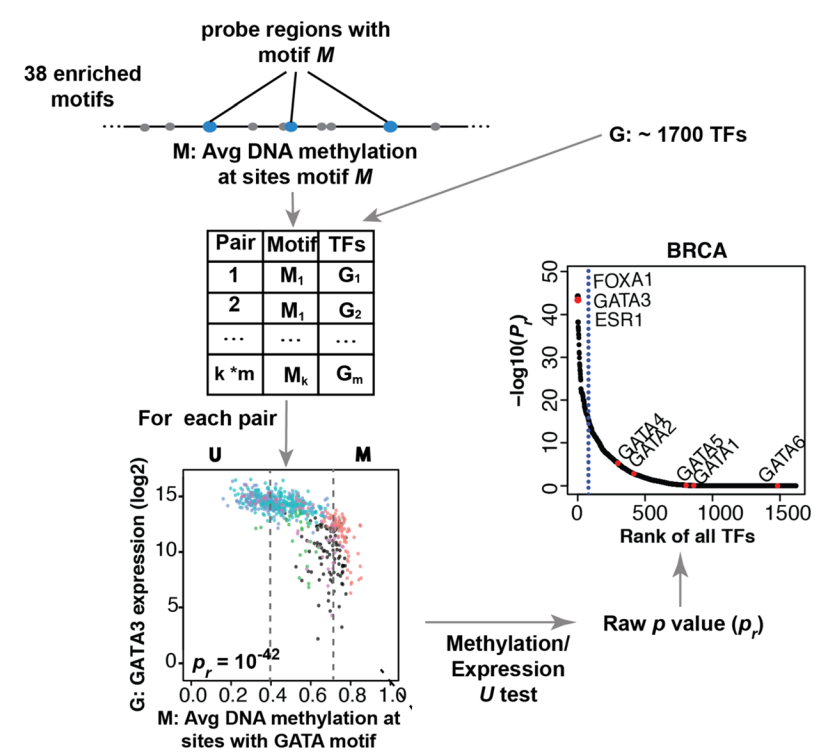
\includegraphics[width=0.7\linewidth]{ELMER/tfrank.png}{\tiny{\\\href{https://genomebiology.biomedcentral.com/articles/10.1186/s13059-015-0668-3}{Yao et al. Genome Biology (2015) 16:105.}}}
 \end{figure}
\end{frame}

\begin{frame}{Step 5: TF scatter plot}
 \begin{figure}
  \centering
  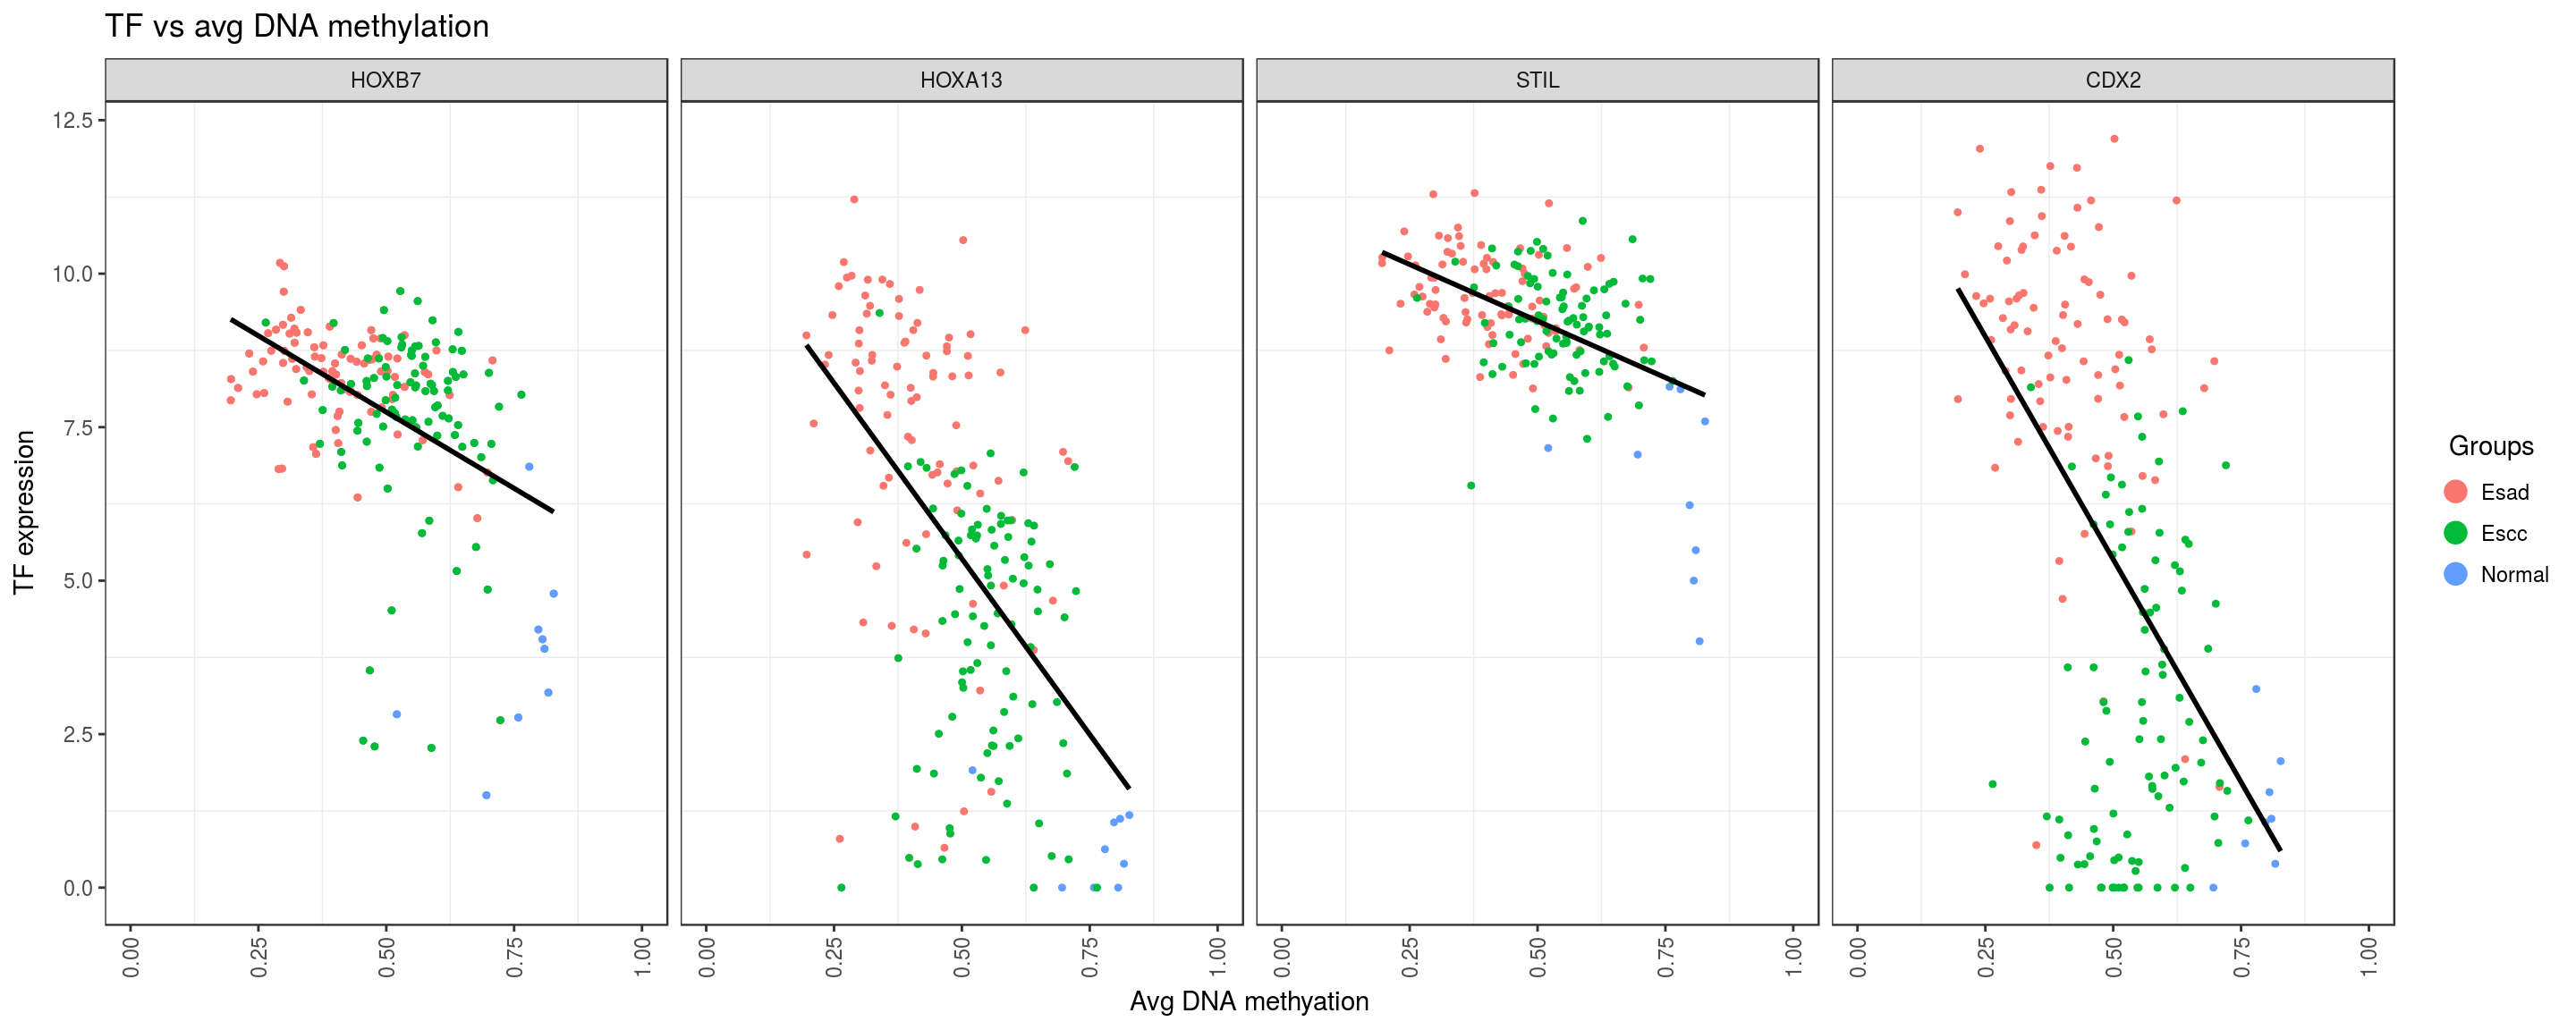
\includegraphics[width=1.0\linewidth]{ELMER/TF_plot_scatter.png}{\tiny{\\HOXB13 motif - Probes hypomethylated in esad vs normal}}
 \end{figure}
\end{frame}

\begin{frame}{Step 5: TF ranking plot}
 \vspace*{-0.5cm}
 \begin{figure}
  \centering
  %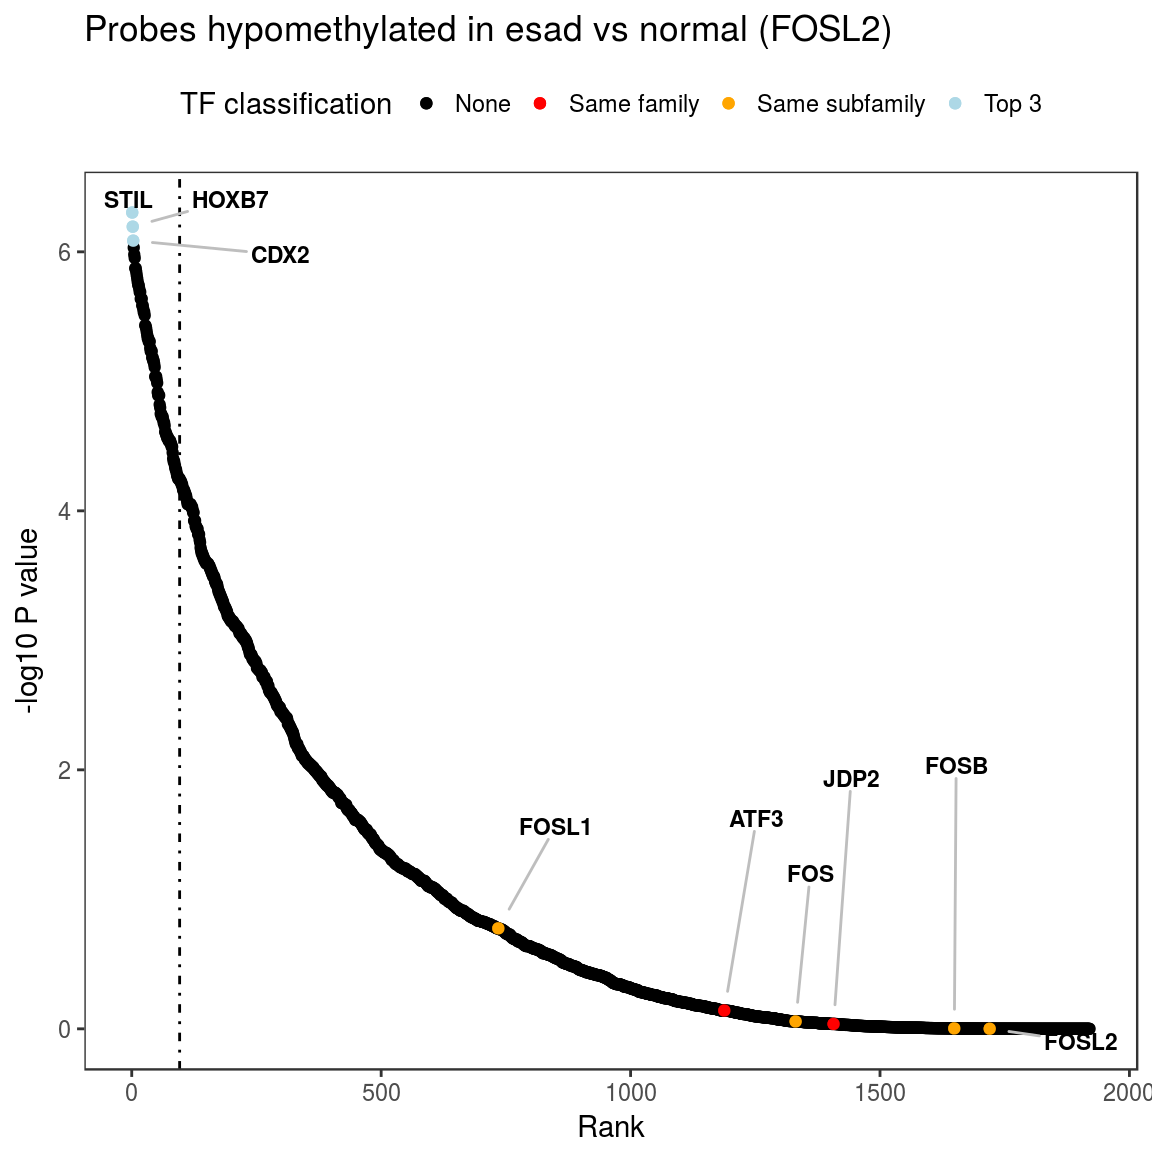
\includegraphics[width=0.45\linewidth]{ELMER/FOS_TF.png}
  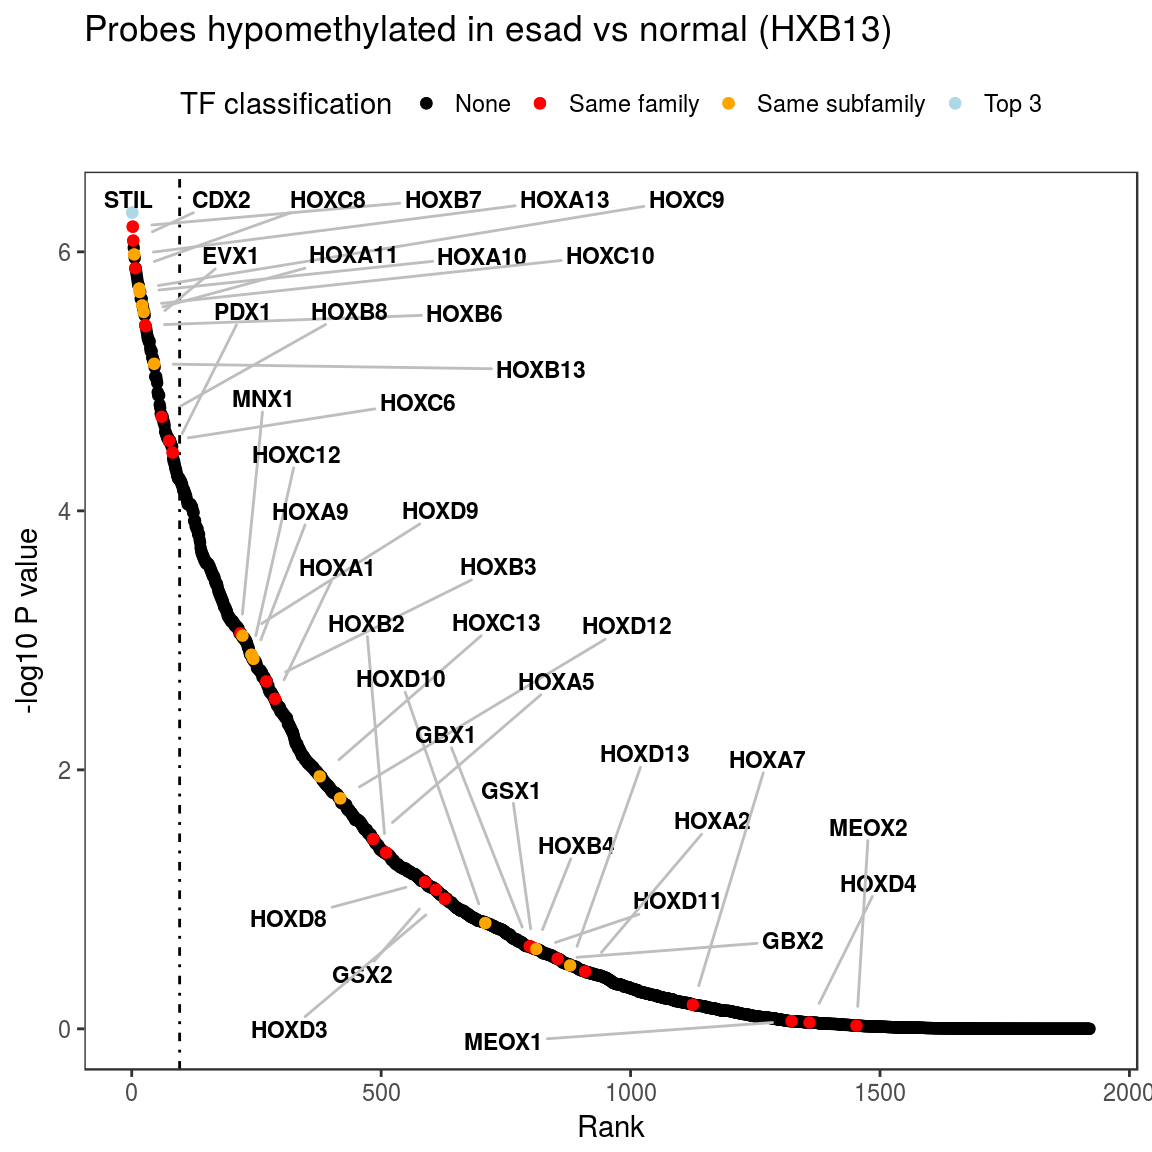
\includegraphics[width=0.7\linewidth]{ELMER/HOX_TF.png}
 \end{figure}
\end{frame}

\begin{frame}{Step 5: TF master regulator table}
 \begin{figure}
  \centering
  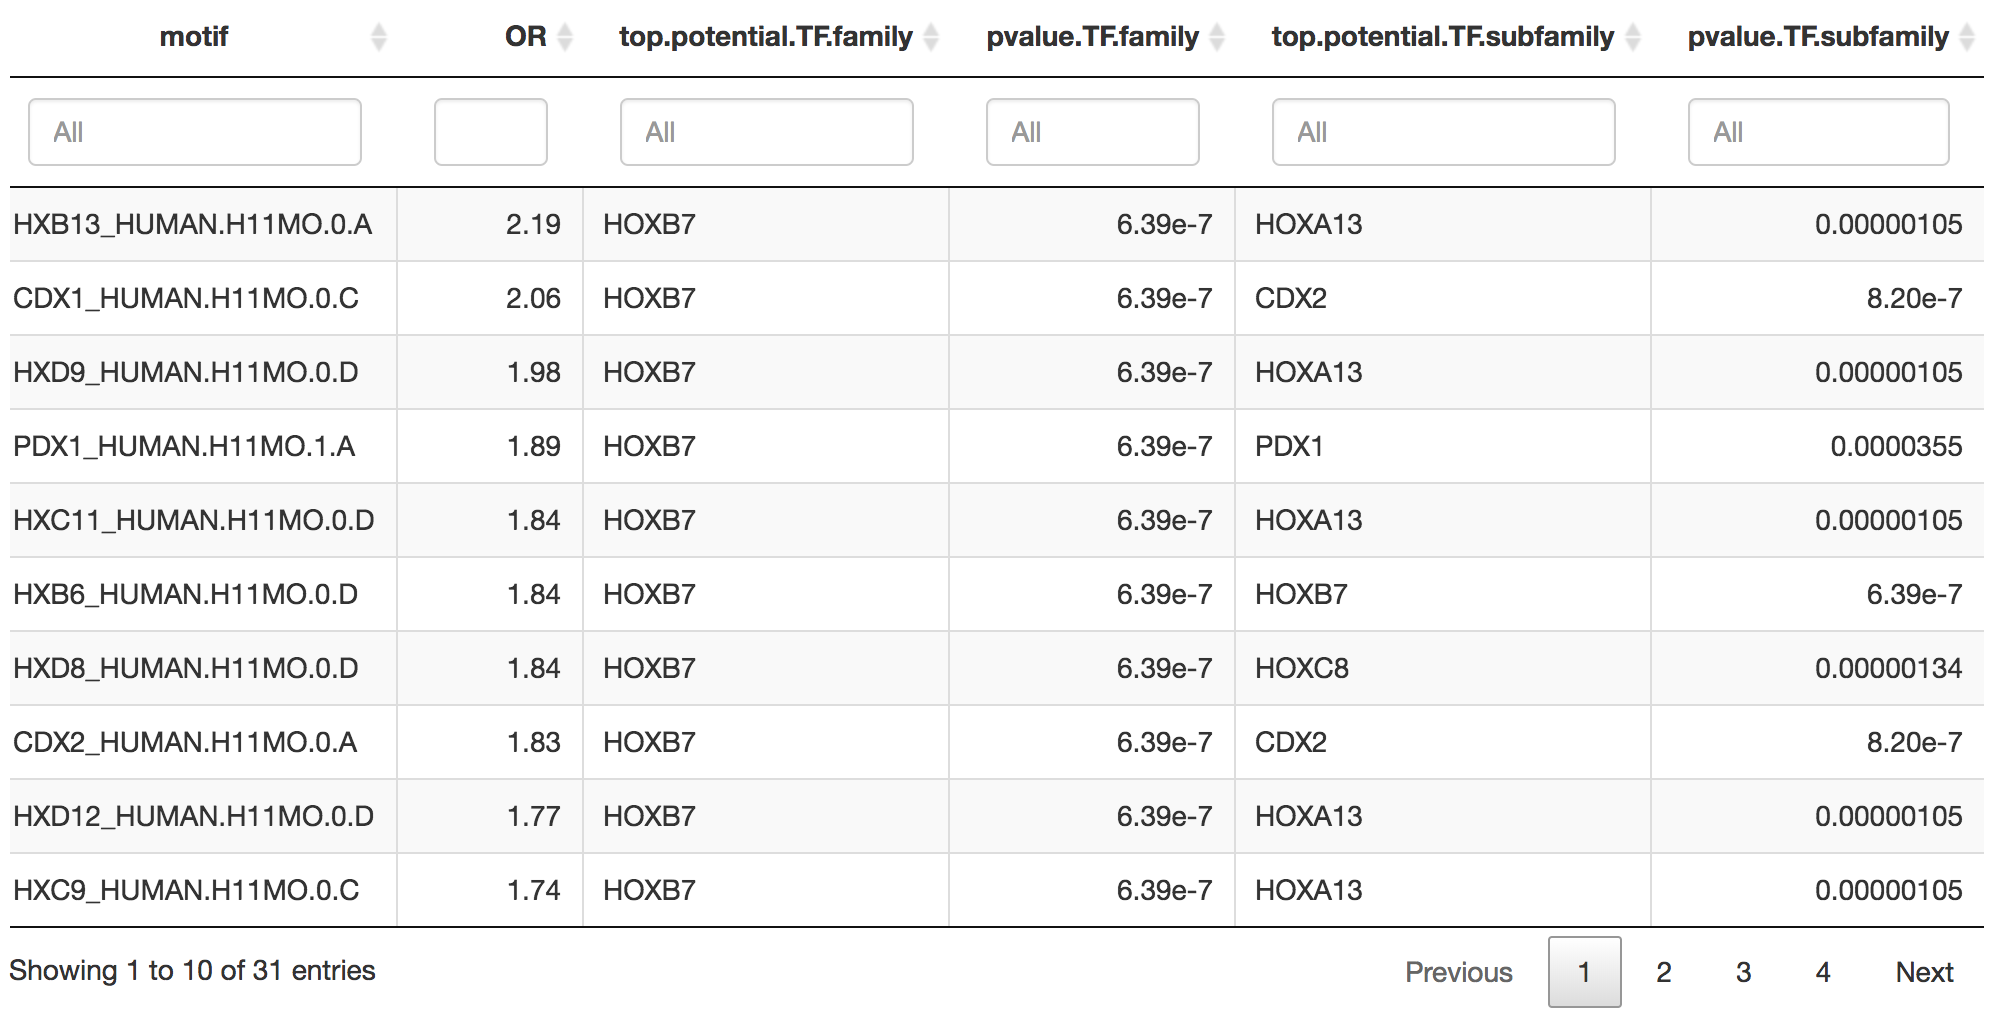
\includegraphics[width=1.0\linewidth]{ELMER/TF_tbl.png}
 \end{figure}
\end{frame}

\begin{frame}{Main differences between ELMER v.1 and v.2}
 \normalsize{
 \begin{table}[h!]
 \centering
 %{\def\arraystretch{2}\tabcolsep=10pt
 \resizebox{\textwidth}{!}{%
 \begin{tabular}{@{}m{4cm}m{5cm}m{7cm}@{}}
 \toprule
 \toprule
 \multicolumn{1}{c}{\textbf{Features}} & \multicolumn{1}{c}{\textbf{ELMER Version 1}} & \multicolumn{1}{c}{\textbf{ELMER Version 2}}   \\ \midrule \midrule
 Primary data structure      & mee object (custom data structure)   & MAE object (Bioconductor data structure) \\ \midrule
 Auxiliary data      & Manually created   & Programmatically created \\\midrule
 Number of human TFs       & 1,982 & 2,014 (Uniprot database)    \\\midrule
 Number of TF motifs      & 91    & 771  (HOCOMOCO v11 database)    \\\midrule
 TF classification &  78 families         & 82 families and 331 subfamilies \newline(TFClass database) \\\midrule
 Analysis performed            & Normal vs tumor samples & Group 1 vs group 2   \\ \midrule
 Statistical grouping            & Unsupervised only & Unsupervised or supervised using labeled groups   \\ \midrule
 TCGA data source      & The Cancer Genome Atlas (TCGA) (not available)      & The NCI's Genomic Data Commons (GDC)     \\\midrule
 Genome of reference      & GRCh37 (hg19)      & GRCh37 (hg19)/GRCh38 (hg38)          \\\midrule
 DNA methylation platforms             & HM450  & EPIC and HM450            \\\midrule
 Graphical User interface (GUI)        & None  & TCGAbiolinksGUI   \\
 \bottomrule
 \end{tabular}
 }
 %}
 \end{table}
 }
\end{frame}


\section{Case of study}

\begin{frame}{Case study: TCGA Breast Invasive Carcinoma (BRCA)}
 \begin{table}[ht!]
  \centering
  \caption{Summary of the available samples in TCGA for BRCA}
  \scriptsize

  \begin{tabular}{p{2.3cm}p{2.4cm}p{2.4cm}p{1cm}}
   \toprule
   Group               & Samples w/ DNA methylation (450K) & Samples w/ gene expression (FPKM-UQ) & Samples w/ both \\ \midrule
   Primary solid Tumor & 791                               & 1102                                 & 778             \\
   Solid Tissue Normal & 96                                & 113                                  & 83              \\
   \bottomrule
  \end{tabular}
 \end{table}

 \begin{table}[ht!]
  \centering
  \caption{Results supervised mode}
  \scriptsize

  \begin{tabular}{p{2.8cm}p{2.4cm}}
   \toprule
   Inferred gene-probe pairs & 2167 \\
   Enriched motifs           & 312  \\
   Regulatory TF factors     & 17   \\
   \bottomrule
  \end{tabular}
 \end{table}
\end{frame}


\begin{frame}{Step 3: Probe-target gene pairs inferred}
\vspace*{-0.5cm}
\begin{figure}
 \centering
   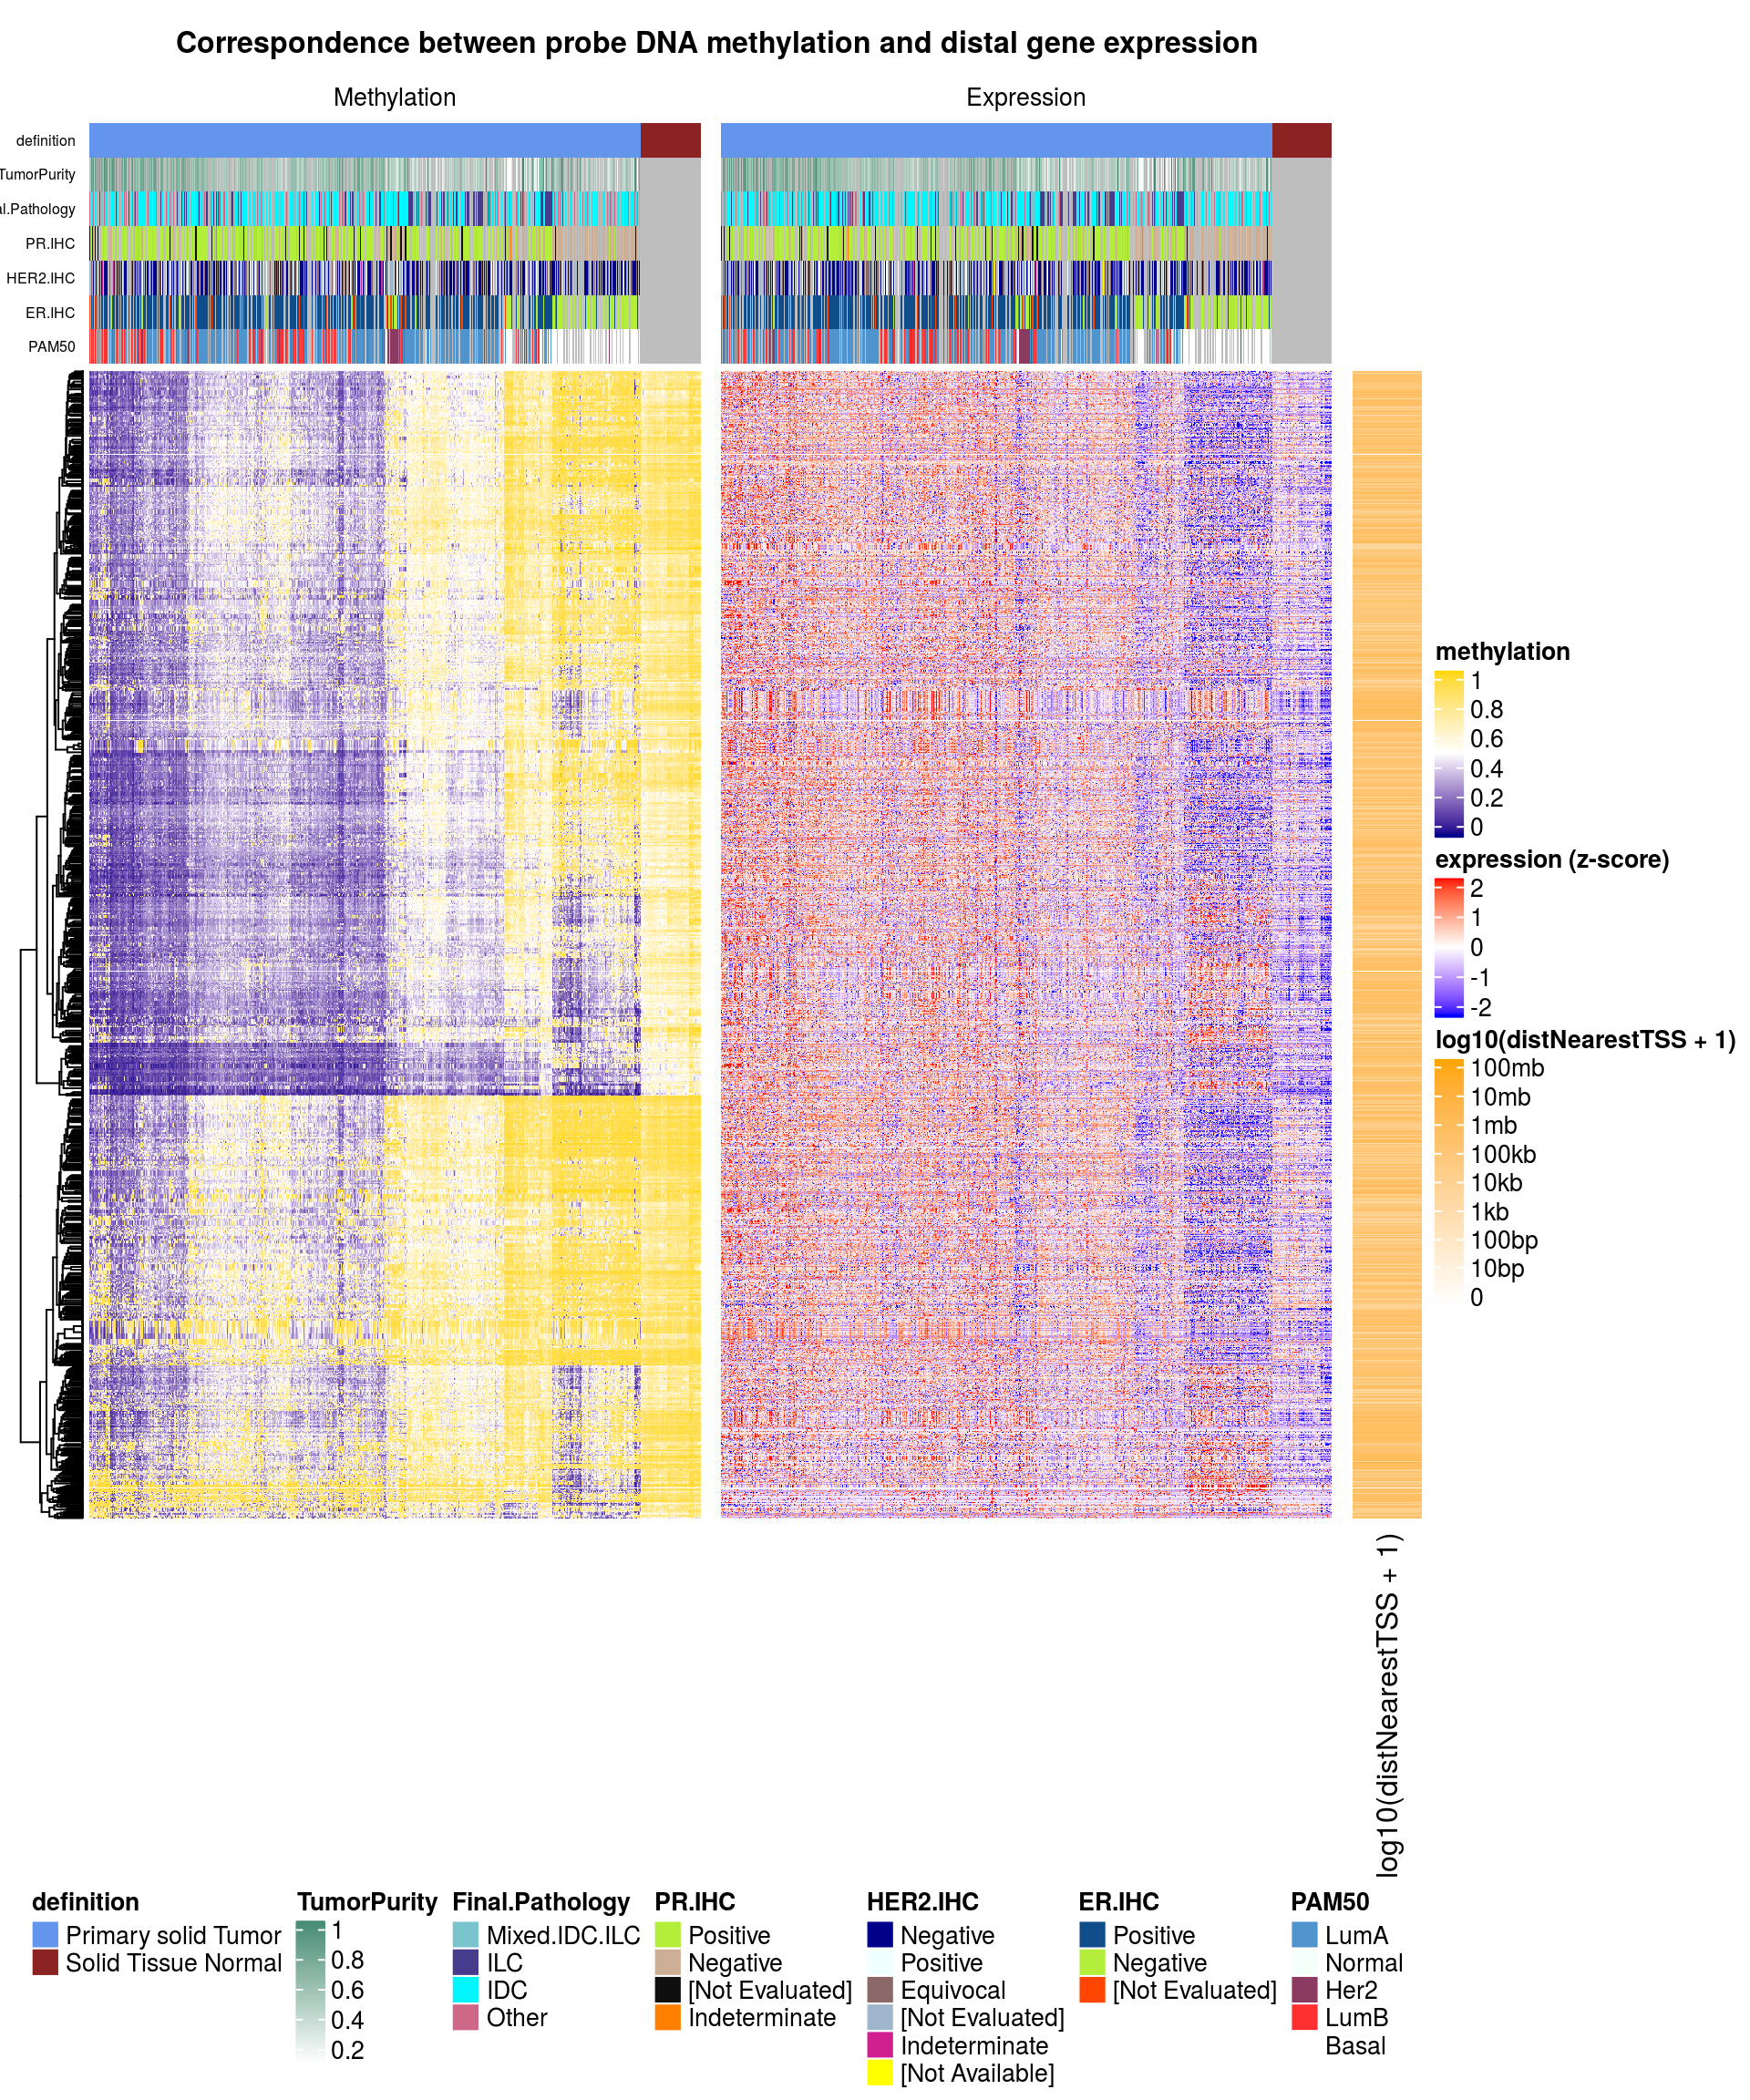
\includegraphics[width=0.75\linewidth]{ELMER/BRCA_heatmap.png}
   \end{figure}
\end{frame}


\begin{frame}{Top enriched motifs}
 \vspace*{-0.3cm}
 \begin{figure}
  \centering
  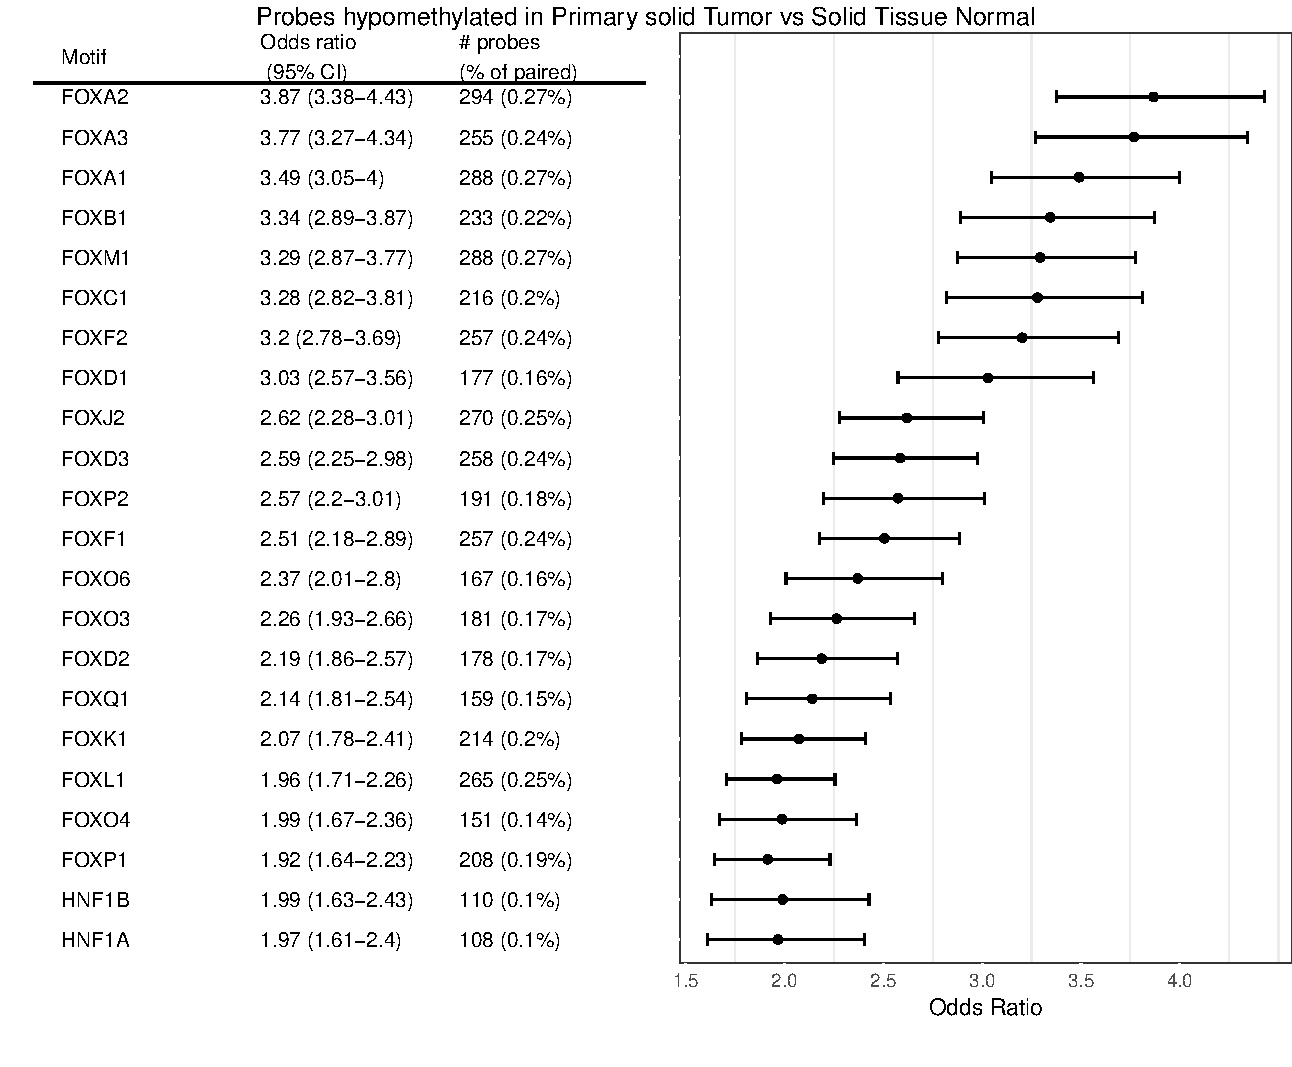
\includegraphics[width=0.85\linewidth]{ELMER/BRCA_unsupervise_OR_table.pdf}
 \end{figure}
\end{frame}


\begin{frame}{TF ranking plot - FOXA2 motif}
 \vspace*{-0.3cm}
 \begin{figure}
  \centering
  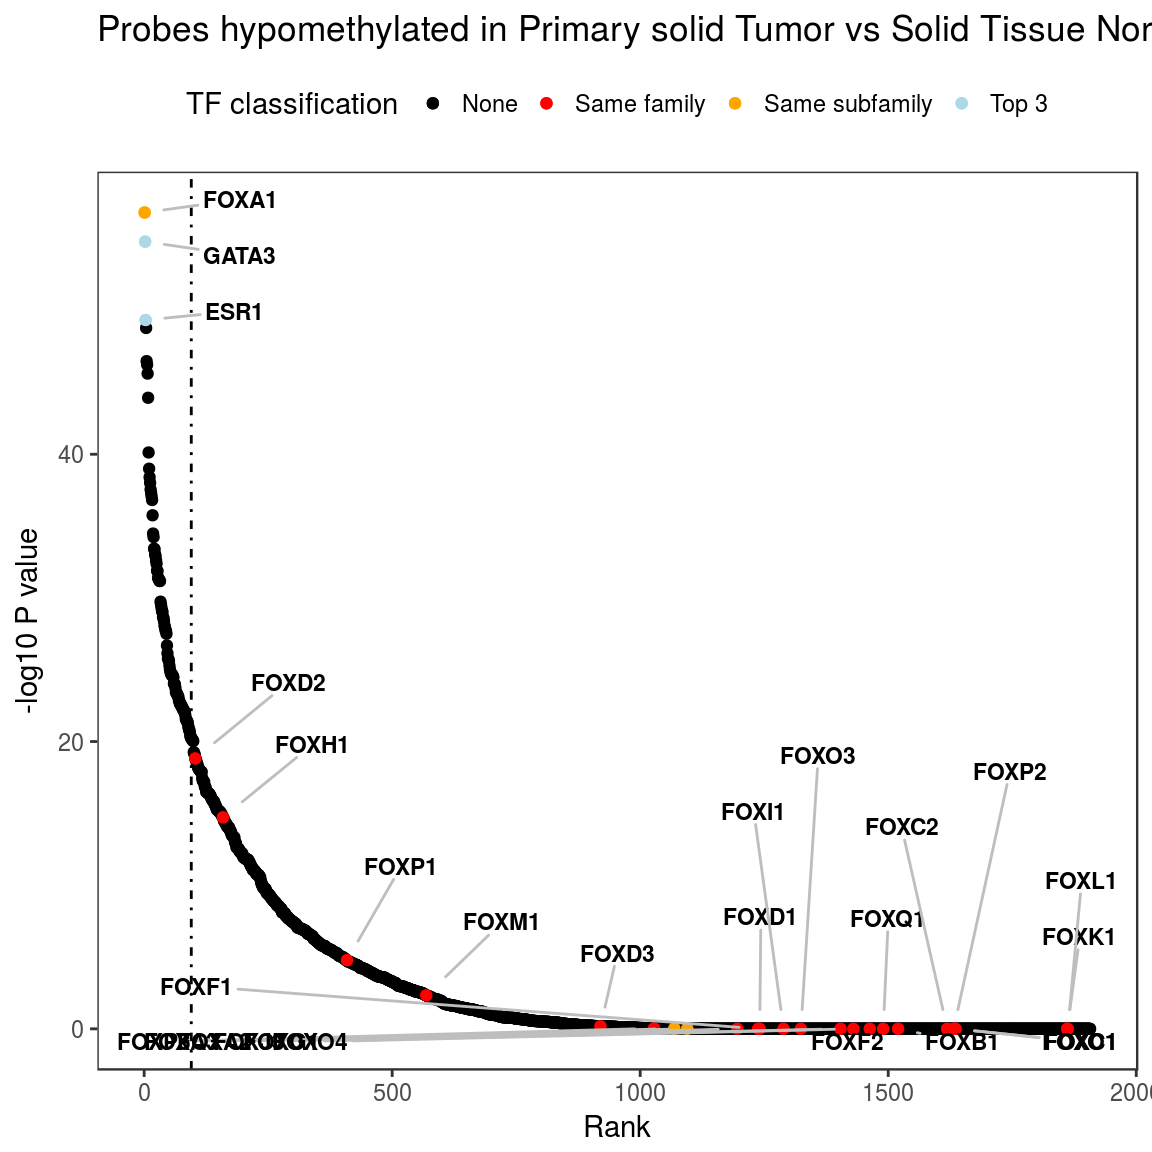
\includegraphics[width=0.7\linewidth]{ELMER/BRCA_TF_rank.png}
 \end{figure}
\end{frame}

\begin{frame}{DNA methylation at motifs vs TF expression}
 \begin{figure}
  \centering
  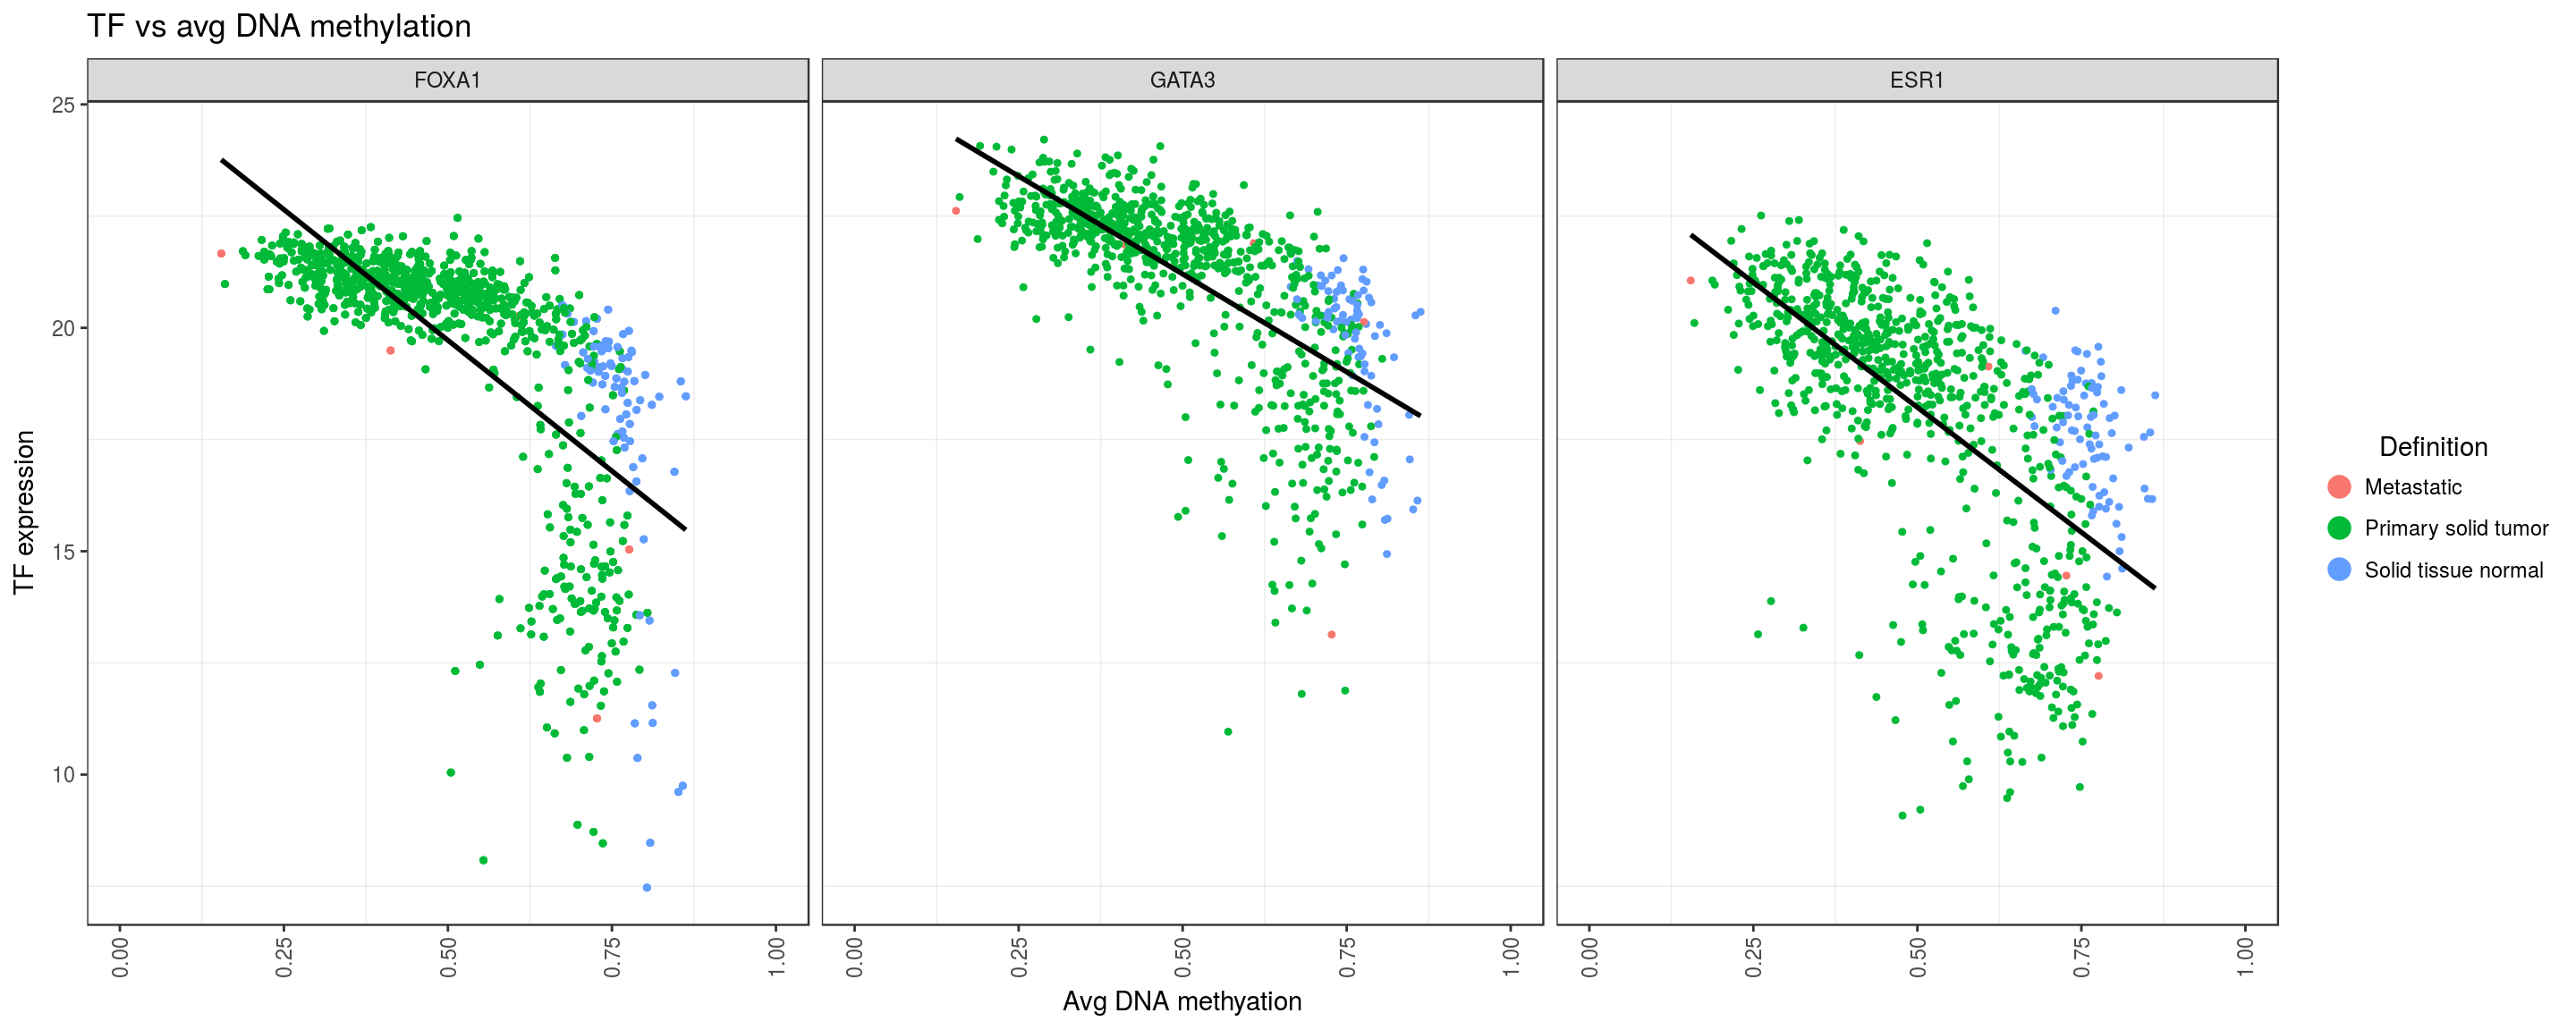
\includegraphics[width=1.0\linewidth]{ELMER/BRCA_TF_scatter.png}
 \end{figure}
\end{frame}


\begin{frame}{Candidate regulatory TF}
 \vspace*{-0.3cm}
 \begin{figure}
  \centering
  \includegraphics[width=0.8\linewidth]{ELMER/paper4.png}\\
  \includegraphics[width=0.8\linewidth]{ELMER/paper1.png}\\
  \includegraphics[width=0.8\linewidth]{ELMER/paper2.png}
  %\includegraphics[width=0.8\linewidth]{paper3.png}
 \end{figure}
\end{frame}

\begin{frame}{Characterization of chromatin state context of enriched probes using FunciVar}
 \vspace*{-0.3cm}
 \begin{figure}[ht!]
  \centering
  \includegraphics[width=0.9\textwidth]{images/1.png}%\tiny{\\Enrichment of paired probes and chromatin states of encode cells. The plot shows enrichment for enhancer active region (EAR), weak enhancer (EWR) and active promoter region (PAR) for MCF-7 cell. }
 \end{figure}
 \pdfnote{remember to say thank you to simon}
 \pdfnote{
  Enrichment of paired probes and chromatin states of encode cells. The plot shows enrichment for enhancer active region (EAR), weak enhancer (EWR) and active promoter region (PAR) for MCF-7 cell.
  Acronyms - AR: Active region, EAR: active enhancer, EWR: Weak Enhancer, EPR: poised enhancer, PAR: active promoter, PWR: Weak Promoter, PPR: poised promoter, PPWR: Weak Poised Promoter, CTCF: architectural complex, TRS: transcribed, HET: heterochromatin, SCR: Polycomb Repressed Silenced
 }
\end{frame}

\begin{frame}{Comparing inferred results with MCF-7 chIA-PET}

 \begin{figure}[ht!]
  \centering
  \includegraphics[width=0.6\textwidth]{ELMER/validation.png}\tiny{\\MCF7 ChIA-PET (Chromatin Interaction Analysis with Paired-End-Tag sequencing) from Li, Guoliang, et al. "Extensive promoter-centered chromatin interactions provide a topological basis for transcription regulation." Cell 148.1 (2012): 84-98. (https://doi.org/10.1016/j.cell.2011.12.014).}
 \end{figure}
\end{frame}

\begin{frame}[plain]{Supervised analysis: BRCA molecular subtypes}
\vspace*{-0.45cm}
 \begin{figure}[ht!]
  \centering
  \includegraphics[width=1.0\textwidth]{ELMER/breastcancer-subtypes.png}\tiny{\\Source: Eric Wong. Available at: http://www.pathophys.org/breast-cancer/. Accessed 25/12/2017.}
 \end{figure}
\end{frame}

\begin{frame}{BRCA supervised analysis}

 \begin{figure}[ht!]
  \centering
  \includegraphics[width=1.0\textwidth]{ELMER/groups.png}
  \includegraphics[width=1.0\textwidth]{ELMER/arguments.png}
 \end{figure}
\end{frame}


\begin{frame}{Supervised analysis: Candidate regulatory TFs }
\vspace*{-0.7cm}
\begin{table}[]
\tiny
\centering
\begin{tabular}{@{}|c|c|c|c|c|c|c|c|c|@{}}
\midrule
\textit{\textbf{TF}} & \textbf{\begin{tabular}[c]{@{}c@{}}LumA \\ (vs basal)\end{tabular}} & \textbf{\begin{tabular}[c]{@{}c@{}}LumB \\ (vs basal)\end{tabular}} & \textbf{\begin{tabular}[c]{@{}c@{}}LumA \\ (vs normal)\end{tabular}} & \textbf{\begin{tabular}[c]{@{}c@{}}LumB \\ (vs normal)\end{tabular}} & \textbf{\begin{tabular}[c]{@{}c@{}}Basal \\ (vs LumA)\end{tabular}} & \textbf{\begin{tabular}[c]{@{}c@{}}Basal \\ (vs LumB)\end{tabular}} & \textbf{\begin{tabular}[c]{@{}c@{}}Basal \\ (vs HER2)\end{tabular}} & \textbf{\begin{tabular}[c]{@{}c@{}}HER2 \\ (vs Basal)\end{tabular}} \\ \midrule
\textit{\textbf{AR}} & x & x & x &  &  &  &  &  \\
\textit{\textbf{BCL11A}} &  &  &  &  & x & x & x &  \\
\textit{\textbf{CEBPB}} &  &  &  &  & x & x & x &  \\
\textit{\textbf{E2F3}} &  &  &  &  &  & x & x &  \\
%\textit{\textbf{ELF5}} &  &  &  &  & x &  &  &  \\
\textit{\textbf{EMX1}} & x & x & x &  &  &  &  &  \\
\textit{\textbf{ESR1}} & x & x & x & x &  &  &  &  \\
\textit{\textbf{ETV6}} &  &  &  &  & x & x & x &  \\
\textit{\textbf{FOXA1}} & x & x & x & x &  &  &  & x \\
%\textit{\textbf{FOXD2}} &  & x &  &  &  &  &  &  \\
\textit{\textbf{FOXP1}} & x & x &  &  &  &  &  & x \\
%\textit{\textbf{GATA2}} & x &  &  &  &  &  &  & x \\
\textit{\textbf{GATA3}} & x & x & x & x &  &  &  & x \\
%\textit{\textbf{GLI1}} & x & x &  &  &  &  &  &  \\
\textit{\textbf{HOXB1}} & x & x &  &  &  &  &  &  \\
\textit{\textbf{HOXB2}} & x & x &  &  &  &  &  & x \\
\textit{\textbf{HOXB3}} &  &  &  &  &  &  &  & x \\
%\textit{\textbf{HOXB6}} &  &  &  &  &  &  &  & x \\
\textit{\textbf{HOXC10}} &  &  &  &  &  &  &  & x \\
%\textit{\textbf{HOXC11}} &  &  &  &  &  &  &  & x \\
\textit{\textbf{KLF5}} &  &  &  &  &  & x & x &  \\
\textit{\textbf{LMX1B}} & x & x & x &  &  &  &  &  \\
%\textit{\textbf{MAZ}} &  &  & x &  &  &  &  &  \\
\textit{\textbf{MNX1}} &  &  &  &  &  &  &  & x \\
%\textit{\textbf{MSX2}} & x & x &  &  &  &  &  &  \\
\textit{\textbf{MYB}} & x &  &  & x &  &  &  &  \\
%\textit{\textbf{MYBL1}} &  &  &  & x &  &  &  &  \\
%\textit{\textbf{MYBL2}} &  &  &  & x & x &  &  &  \\
%\textit{\textbf{NFATC4}} & x &  &  &  &  &  &  &  \\
%\textit{\textbf{NFIB}} &  &  &  &  & x &  &  &  \\
\textit{\textbf{NFIL3}} &  &  &  &  & x & x &  &  \\
%\textit{\textbf{NR2E3}} & x & x &  &  &  &  &  &  \\
%\textit{\textbf{OVOL2}} &  &  & x &  &  &  &  &  \\
%\textit{\textbf{PATZ1}} &  & x & x &  &  &  &  &  \\
\textit{\textbf{PBX1}} &  & x &  & x &  &  &  &  \\
%\textit{\textbf{POU2F1}} &  &  & x & x &  &  &  &  \\
%\textit{\textbf{PGR}} & x & x &  &  &  &  &  &  \\
\textit{\textbf{RARA}} & x & x & x &  &  &  &  &  \\
\textit{\textbf{RUNX3}} &  &  &  &  & x & x &  &  \\
\textit{\textbf{SOX8}} &  &  &  &  &  & x & x &  \\
\textit{\textbf{SOX9}} &  &  &  &  &  & x & x &  \\
\textit{\textbf{SOX11}} &  &  &  &  & x & x &  &  \\
%\textit{\textbf{ZNF281}} &  &  & x & x &  &  &  &  \\
%\textit{\textbf{ZNF423}} & x &  &  &  &  &  &  &  \\
\textit{\textbf{ZNF467}} & x & x & x &  &  &  &  &  \\
\textit{\textbf{ZIC1}} &  &  &  &  & x & x & x &  \\ \bottomrule
\end{tabular}
\end{table}
\end{frame}




\begin{frame}{TF master regulator: LumA}

 \begin{figure}[ht!]
  \centering
  \includegraphics[width=1.0\textwidth]{ELMER/FOXA3_motif.png}
  \caption{\label{fig:chiapet} FOXA1 and top3 TF expression vs avg DNA methylation of paired enriched probes for FOXA3 motif - Probes hypomethylated in LumA vs Normal-like}
 \end{figure}
\end{frame}

\begin{frame}{TF master regulator: Basal}

 \begin{figure}[ht!]
  \centering
  \includegraphics[width=1.0\textwidth]{ELMER/SOX10_TF.png}
  \caption{\label{fig:chiapet} SOX11 and top3 TF expression vs avg DNA methylation of paired enriched probes for SOX10 - Probes hypermethylated in LumA vs Basal}
 \end{figure}
\end{frame}


\begin{frame}{TF master regulator: Basal}

 \begin{figure}[ht!]
  \centering
  \includegraphics[width=1.0\textwidth]{ELMER/SOX11_basal.png}
  \includegraphics[width=1.0\textwidth]{ELMER/SOX9_2.png}
  \includegraphics[width=1.0\textwidth]{ELMER/SOX9_1.png}
  \includegraphics[width=1.0\textwidth]{ELMER/GATA3.png}
  \includegraphics[width=1.0\textwidth]{ELMER/cofactors.png}
     \end{figure}
\end{frame}

\section{Glioma analysis}


\begin{frame}{Glioma analysis: glioma subgroups}
\vspace{-0.5cm}
 \begin{figure}[ht!]
  \centering
  \includegraphics[width=0.9\textwidth]{glioma/figure1.pdf}{\tiny{\\Source: Ceccarelli, Michele, et al. Cell 164.3 (2016): 550-563. DOI: http://dx.doi.org/10.1016/j.cell.2015.12.028}}
 \end{figure}
\end{frame}

\begin{frame}{G-CIMP supervised analysis}

 \begin{figure}[ht!]
  \centering
  \includegraphics[width=1.0\textwidth]{glioma/groups.png}
  \includegraphics[width=1.0\textwidth]{glioma/arguments.png}
 \end{figure}
\end{frame}


\begin{frame}{Differentially methylated distal probes}
\vspace{-0.5cm}
 \begin{figure}[ht!]
  \centering
  \includegraphics[width=1.0\textwidth]{glioma/volcano.png}
  \caption{}
 \end{figure}
\end{frame}

\begin{frame}{Paired gene-probes}
\vspace{-0.5cm}
 \begin{figure}[ht!]
  \centering
  \includegraphics[width=0.8\textwidth]{glioma/heatmap.png}
  \caption{}
 \end{figure}
\end{frame}


\begin{frame}{Enriched motifs}
%\vspace{-0.5cm}
 \begin{figure}[ht!]
  \centering
  \includegraphics[width=0.8\textwidth]{glioma/or.png}
 \end{figure}
\end{frame}

\begin{frame}{Candidate master regulator Transcription Factors (TF) }
\begin{block}{Top TFs}
  \begin{itemize}
    \item  HOXD13
    \item  HMX3
    \item  ZSCAN16
    \item  SOX11
    \item  PAX3
    \item  FOXM1
  \end{itemize}
\end{block}
\end{frame}

\begin{frame}{HOXD13}
\vspace{-0.5cm}
 \begin{figure}[ht!]
  \centering
  \includegraphics[width=1.0\textwidth]{glioma/paper_HOXD13b.png}
 \end{figure}
\end{frame}

\begin{frame}{FOXM1 and PAX3}
\vspace{-0.5cm}
 \begin{figure}[ht!]
  \centering
  \includegraphics[width=0.8\textwidth]{glioma/paper_FOXM1.png}
  \includegraphics[width=0.8\textwidth]{glioma/paper_pax3.png}
  \includegraphics[width=0.8\textwidth]{glioma/paper_SOX11.png}
 \end{figure}
\end{frame}

\begin{frame}{SOX11}
 \begin{figure}[ht!]
  \centering
  \includegraphics[width=1.0\textwidth]{glioma/paper_SOX11.png}
 \end{figure}
\end{frame}


\begin{frame}{Next steps: TF knockdown}
 \begin{figure}[ht!]
  \centering
  \includegraphics[width=1.0\textwidth]{glioma/knockdown_TF_ESCA.pdf}
  \caption{Candidate master regulator Transcription Factors (TF) knockdown in the SKGT4 human esophageal adenocarcinoma cell line. Figure produced by Dr. Dechen Lin.}
 \end{figure}
\end{frame}

\section{Conclusion}
\begin{frame}{Conclusion}
\begin{block}{Conclusion}
  \begin{itemize}
    \item  Tools were able to provide methods for (epi) genomics integrative analysis
    using data from several databases.
    \item  Several genes identified using those tools are consistent with literature.
  \end{itemize}
\end{block}
\begin{block}{Future works}
  \begin{itemize}
    \item Extend ELMER algorithm to work with regions (WGBS).
    \item Provided a processing pipeline for WGBS data.
    \item Use mutation information instead of DNA methylation
to identify regulatory regions mutated that might have affected the
regulation of a upstream/downstream genes.
    \item Improve results mining through automatically created reports.
  \end{itemize}
\end{block}
\end{frame}

\begin{frame}{Results: First authorship - articles, software and material online}
\begin{thebibliography}{10}
\tiny
\setbeamertemplate{bibliography item}[article]
\bibitem{EBU2011}
Tiago Chedraoui Silva*, Antonio Colaprico*, et al.
\newblock TCGAbiolinks: An R/Bioconductor package for integrative analysis of TCGA data. Nucleic Acids Res.,
\newblock Nucleic acids research, p.gkv1507, 2015

%\beamertemplateonlinebibitems
\beamertemplatearticlebibitems
\bibitem{F10002016}
Silva TC, Colaprico A, Olsen C et al.
\newblock TCGA Workflow: Analyze cancer genomics and epigenomics data using Bioconductor packages
\newblock  F1000Research 2016, 5:1542

\beamertemplatearticlebibitems
\bibitem{GUI}
Silva, Tiago C., et al.
\newblock "TCGAbiolinksGUI: A graphical user interface to analyze GDC cancer molecular and clinical data."
\newblock bioRxiv (2017): 147496.

\setbeamertemplate{bibliography item}[aticle]
\bibitem{ELMERv2}
Silva, Tiago Chedraoui, et al.
\newblock "Enhancer Linking by Methylation/Expression Relationships with the R package ELMER version 2."
\newblock  bioRxiv (2017): 148726.

\beamertemplateonlinebibitems
\bibitem{F10002016}
Workflow:
\newblock TCGA Workflow: Analyze cancer genomics and epigenomics data using Bioconductor packages\\
 https://www.bioconductor.org/help/workflows/TCGAWorkflow/

\beamertemplateonlinebibitems
\bibitem{workshop}
Workshop:
\newblock Integrative analysis workshop with TCGAbiolinks and ELMER\\ https://bioinformaticsfmrp.github.io/Bioc2017.TCGAbiolinks.ELMER/index.html

\setbeamertemplate{bibliography item}[online]
  \bibitem{EBU2011}
  Softwares:
  \newblock http://bioconductor.org/packages/TCGAbiolinksGUI/\\ http://bioconductor.org/packages/TCGAbiolinks/\\ http://bioconductor.org/packages/ELMER/

  %	\beamertemplatearticlebibitems
  %	\bibitem{EBU2011}
  %S. B. Baylin and P. A. Jones.
  %	\newblock A decade of exploring the cancer epigenome - biological and translational implications.
  %	\newblock Nat. Rev. Cancer, 11(10):726–734, Oct 2011.

 \end{thebibliography}
\end{frame}

\begin{frame}{Results: Co-authorship - articles and software}
\begin{thebibliography}{10}
\tiny


\beamertemplatearticlebibitems
\bibitem{GUI}
M Ceccarelli, et al.
\newblock Molecular profiling reveals biologically discrete subsets and pathways of progression in diffuse glioma
\newblock Cell, 2016

\beamertemplatearticlebibitems
\bibitem{F10002016}
Malta, Tathiane M., et al.
\newblock Glioma CpG island methylator phenotype (G-CIMP): biological and clinical implications
\newblock Neuro-oncology (2017).

\setbeamertemplate{bibliography item}[aticle]
\bibitem{ESCA}
Lin, De-Chen, et al.
\newblock Identification of distinct mutational patterns and new driver genes in oesophageal squamous cell carcinomas and adenocarcinomas
\newblock Gut, pp.gutjnl-2017.

\setbeamertemplate{bibliography item}[aticle]
\bibitem{ESCA}
Cava, Claudia, et al.
\newblock SpidermiR: An R/Bioconductor Package for Integrative Analysis with miRNA Data
\newblock International journal of molecular sciences. 2017 Jan 27;18(2):274.


\setbeamertemplate{bibliography item}[online]
  \bibitem{EBU2011}
  Softwares:
  \newblock 	http://bioconductor.org/packages/SpidermiR/
 \end{thebibliography}
\end{frame}

\begin{frame}{Acknowledgments}
 %\vspace{-0.5cm}
 \begin{columns}[T]
  \begin{column}{0.5\textwidth}
   \begin{block}{University of São Paulo}
    \begin{itemize}
      \item  Houtan Noushmerh
      \item  Camila Ferreira de Souza
      \item  Tathiane Malta
    \end{itemize}
   \end{block}
  \end{column}
  \begin{column}{0.5\textwidth}
   \vspace{0.9cm}
   \includegraphics[width=0.4\linewidth]{logo/usp.png}
  \end{column}
 \end{columns}

 \vspace{0.2cm}
 \begin{columns}[T]
  \begin{column}{0.5\textwidth}
   \begin{block}{Cedars-Sinai}
    \begin{itemize}
     \item Ben Berman
     \item Simon Coetzee
     \item Dennis Hazelett
     \item Nicole Yeager
     \item Dechen Lin
    \end{itemize}
   \end{block}
  \end{column}
  \begin{column}{0.5\textwidth}
   \vspace{1.5cm}
   \includegraphics[width=1.0\linewidth]{cedars.png}
  \end{column}
 \end{columns}

\end{frame}


\begin{frame}{References}
 \begin{thebibliography}{10}
  \tiny
  \beamertemplatebookbibitems
  \bibitem{Oppenheim2009}
  Ginsburg, Geoffrey S., and Huntington F. Willard.
  \newblock Genomic and personalized medicine.
  \newblock  Vol. 1. Academic Press, 2008.

  \beamertemplatearticlebibitems
  \bibitem{F10002016}
  Silva TC, Colaprico A, Olsen C et al.
  \newblock TCGA Workflow: Analyze cancer genomics and epigenomics data using Bioconductor packages
  \newblock  F1000Research 2016, 5:1542

  \beamertemplatearticlebibitems
  \bibitem{EBU2011}
  H. Noushmehr, D. J. Weisenberger, et al.
  \newblock Identification of a CpG island methylator phenotype that defines a distinct subgroup of glioma.
  \newblock Cancer Cell, 17(5):510–522, May 2010.

  \beamertemplatearticlebibitems
  \bibitem{EBU2011}
  S. Sharma, T. K. Kelly, and P. A. Jones.
  \newblock Epigenetics in cancer.
  \newblock  Carcinogenesis, 31(1):27–36, Jan 2010.

  \beamertemplatearticlebibitems
  \bibitem{EBU2011}
  Tiago Chedraoui Silva*, Antonio Colaprico*, et al.
  \newblock TCGAbiolinks: An R/Bioconductor package for integrative analysis of TCGA data. Nucleic Acids Res.,
  \newblock Nucleic acids research, p.gkv1507, 2015

  \beamertemplatearticlebibitems
  \bibitem{EBU2011}
  Ceccarelli M, Barthel FP, Malta TM, Sabedot TS, Salama SR, et al. . Cell,
  \newblock Molecular profiling reveals biologically discrete subsets and pathways of progression in diffuse glioma
  \newblock Cell, 164(3):550-563, 2016


  %	\beamertemplatearticlebibitems
  %	\bibitem{EBU2011}
  %S. B. Baylin and P. A. Jones.
  %	\newblock A decade of exploring the cancer epigenome - biological and translational implications.
  %	\newblock Nat. Rev. Cancer, 11(10):726–734, Oct 2011.

 \end{thebibliography}
\end{frame}

\begin{frame}{Thank you for your attention!}
 \vspace*{2.5cm}
 \centering
 \Huge{Any questions?}
\end{frame}


%-=-=-=-=-=-=-=-=-=-=-=-=-=-=-=-=-=-=-=-=-=-=-=-=
%
%	SECTION: Conclusion
%
%-=-=-=-=-=-=-=-=-=-=-=-=-=-=-=-=-=-=-=-=-=-=-=-=


\end{document}
